% Created with jtex v.1.0.20
\documentclass[a4paper,11pt,oneside]{book}
\usepackage[top=2cm, bottom=2cm, left=2cm, right=2cm]{geometry}
\usepackage[T1]{fontenc}
\usepackage[utf8]{inputenc}
\usepackage{lmodern}
\usepackage{graphicx}
\usepackage{caption}
\usepackage{natbib}
\usepackage{xcolor}
\usepackage{changepage}
\usepackage{framed}
\usepackage{hyperref}
\usepackage{amssymb}
\bibliographystyle{abbrvnat}

% Make list items more compact
\usepackage{enumitem}
\setlist[itemize]{noitemsep, topsep=0pt}

%%%%%%%%%%%%%%%%%%%%%%%%%%%%%%%%%%%%%%%%%%%%%%%%%%
%%%%%%%%%%%%%%%%%%%%  imports  %%%%%%%%%%%%%%%%%%%
\usepackage{amsmath}
%%%%%%%%%%%%%%%%%%%%%%%%%%%%%%%%%%%%%%%%%%%%%%%%%%


\hypersetup{
  colorlinks,
  linkcolor={black},
  citecolor={black},
  urlcolor={black}
}

% Style quotes
\definecolor{darkblue}{rgb}{0.0, 0.0, 0.55}
\definecolor{quoteshade}{rgb}{0.95, 0.95, 1}
\renewenvironment{quote}{%
  \def\FrameCommand{%
    \hspace{1pt}%
    {\color{darkblue}\vrule width 2pt}%
    {\color{quoteshade}\vrule width 4pt}%
    \colorbox{quoteshade}%
  }%
  \MakeFramed {\advance\hsize-\width \FrameRestore}%
  \noindent\hspace{-8pt}% disable indenting first paragraph
  \begin{adjustwidth}{0pt}{0pt}% adjust as needed
  \vspace{2pt}\vspace{2pt}%
}
{%
  \vspace{2pt}\end{adjustwidth}\endMakeFramed%
}

\title{\Huge \textbf{What kind of thing is a planet?}}
\author{\textsc{Rohan Scott Byrne}}

\begin{document}
\sloppy

\frontmatter
\maketitle

\tableofcontents
% \listoffigures
% \listoftables

\mainmatter

% \include{preface.tex}
% \include{acknowledgements.tex}

\cite{Sarma2008-wu}

\section{Review and Theory}

The purpose of this study is to deduce what underlying parameters most strongly control a planet's choice of tectonic mode. The fundamental question regards the existence or otherwise of a well-defined `tectonic phase diagram' in which primarily temperature defines the proper global geodynamic regime at any given time. Phase spaces are defined by their phase transitions, and in the field of planetary geodynamics, only one such transition is well-attested and amenable to study: the emergence on Earth of plate tectonics from an earlier pre-tectonic state of disputed character. The Early Earth is therefore key to the larger question of tectonic modality.

In this review chapter, we will present a brief history of scholarship on the topic, summarise the chief lines of evidence, and discuss the leading hypotheses regarding the divergent fates of Earth and our most familiar planetary cousins. Our line of inquiry will be illustrated with some simple one-dimensional modelling. We will not discuss in detail the analytical and numerical intricacies of the problem at hand, which will instead be related as appropriate in the prefacing remarks of the relevant results chapters (Chapters 3, 4, 5, \& 6); nor will we provide much background or context for our methodological approach, which is treated separately (Chapter 2 \& Chapter 7).

\subsection{Planets from first principles}

Our subject is planets - but what is a planet?

According to the International Astronomical Union highly-publicised ruling of 2006 \cite{International_Astronomical_Union2006-ft}, ``a planet is a celestial body that; 1) is in orbit around a sun, 2) has sufficient mass to have a nearly round shape, 3) has ``cleared the neighborhood'' around its orbit.'' Under this rubric, Pluto, Charon, Eris, and other icy worlds of the outermost solar system are disqualified. Indeed, the rationale for the IAU's opinion was that any broader definition would result in a categorical calamity: potentially hundreds of new worlds would achieve the mantle of `planet', including many that at the time seemed unlikely to be of much significance or interest \cite{Sarma2008-wu}, creating needless public and academic `annoyance' \cite{Basri_2006} \cite{Basri2006-vw}.

The IAU's ruling sparked an impressive global backlash, including an attempt by lawmakers to quash the revision \cite{Zielinski2007-fv} and various pleas for celebrity astronomers to intercede \cite{Tyson2009-oe}. The case has even become a niche topic of sociological literature, with papers discussing its effect on children \citet{Jarman2009-ms, Broughton2013-wz} and its impact on popular perceptions of the credibility of astronomy \citet{Christensen2007-xw, Messeri2010-wo}.

In the immediate aftermath, a petition of over 300 signatures from attendees at the IAU meeting itself protested the new classification, which had been decided by a partial convention of the union rather than a general colloquium, perhaps to avoid protest \cite{Cartlidge2006-oe}. Alan Stern, the director of the New Horizons mission to the outer solar system, quickly became one of the highest-profile advocates for revising or ignoring the IAU opinion \cite{Hogan2006-aw}. He and his colleagues have since developed a so-called `geophysical definition' which is now the standard at NASA \cite{Runyon2017-rz}: ``A planet is a sub-stellar mass body that has never undergone nuclear fusion and that has sufficient self-gravitation to assume a spheroidal shape adequately described by a triaxial ellipsoid regardless of its orbital parameters.''

Stern's definition is a profound revision of the cosmos, but one which is well-argued and well-suited to the purposes of planetary scientists. Under Stern's mandate, not only Pluto and Eris, but also the asteroid belt objects Ceres and Vesta, as well as various `satellite planets' - Earth's moon, Pluto's partner Charon, and most of the satellites of the outer gas giants - all would be considered equally as planets. Such an expansion puts the geophysical, atmospheric, and climatic aspects of planets front and centre, above and beyond their orbital or formational histories. It sets the stage epistemologically for a fundamental deepening of our understanding of the unique processes that govern sub-stellar objects in our universe, and - as we will discuss later (Chapter 8) - may be regarded in retrospect as a milestone event in the birth of a new field of focussed, integrated, holistic planetary science.

\subsection{Heat and geometry: planetary basics}

The geophysical definition of a planet provides some clarification on what should and what shouldn't be included as essential considerations of our topic. A planet is a gravitationally-bound ellipsoidal object, not currently or formerly made of plasma, surrounded by mostly empty space. Such a definition has some immediate implications. The chemical and gravitational prescriptions of Stern's definition provide an upper and lower spatial scale respectively: anywhere from the radius of Mimas, at 200 km the smallest rounded body in the solar system \cite{Lodders1998-dj}, to the radius of Jupiter, about 70,000 km, above which any additional mass tends to be compressed without increasing planet size \cite{Basri2006-vw}. It implies a temporal scale too: between the atmospheric (hours) and geological (gigayear) timescales.

Other implicit constraints are more subtle. Because a planet is qualified by its shape - a function of mass and matter - it is parsimonious to stipulate that these quantities are connate to each planet and cannot be changed. Of course, in reality, such changes do occur: consider the formation of Earth's moon from a putative impact with a Mars-sized planetoid in the Hadean \cite{Canup2012-nz}, or the hypothesised delivery to Earth of a significant mass of volatiles by icy planetoids \cite{Owen2000-ze}. In the system outlined here, however, such events would be considered `catastrophic' - outside of the prescribed spatiotemporal scales of the subject, and violating the prescribed conservative quantities of the problem; in essence, such a calamity would be considered the `death' of the original planet and the `birth' of a new one.

There are also more sustained violations: erosion of planetary atmospheres into space, for example \citet{Perez_de_Tejada1992-qq, Kulikov2006-pc}, or the capture of solar protons in the aurorae \cite{Rees1982-vr}, or the ongoing low-level exchange of meteoroids between Earth and Mars \cite{Melosh1993-cb}. Such endemic exceptions, however, plague all systems; hence we will dub them `pathological', requiring careful handling but not deference.

Planets, then, can be said to be spheroidal, sub-stellar objects of a fixed mass and bulk chemistry. Within these parameters, however, there are considerable degrees of freedom:

\begin{itemize}
\item The geometric characters of the spheroid can change - eccentricity, radius, and obliquity - with consequences for the centre of mass, the gravitational field, and the tidal coupling of the planet with any extra-planetary systems.


\item The distribution of mass can change, anywhere between the extremes of an arbitrarily thin hollow shell and an arbitrarily dense core, with consequences for the moment of inertia and rate of rotation as well as the gravitational field and the gravitational binding energy. The total mass, of course, cannot change - this would be `catastrophic' - hence the gravitational pull of a planet at a sufficient distance above the surface is fixed.


\item The angular velocity of the planet can change due to internal forces and geometric transformations. Angular momentum can also change, though necessarily only by interactions with extra-planetary bodies: when these interactions are periodic, systematic, and persistent over geological time, they may be parameterised as an intrinsic forcing within the planet; otherwise, they may be considered `pathological' (if frequent) or `catastrophic' (if infrequent) exceptions, outside the intrinsic scope of the problem.


\item The chemical makeup of the planet can change. Indeed, all the degrees of freedom within any constituent molecules of a planet are available as degrees of freedom of the planet as a whole, as are all the possibilities for the breaking of old bonds and the forging of new ones.


\item The isotopic makeup of a planet can change, albeit largely without consequence for bulk chemistry - hence their enormous analytical utility as tracers and monitors for Earth sciences. Earth is overwhelmingly composed of less than 300 stable nuclides \cite{Thoennessen2011-jq}.


\item The elemental inventory of a planet can change; here, however, we must be careful. The decay of short-lived radioactive nuclides like Uranium-235 and Thorium-232 into daughter elements are significant to the system; the decays of extremely long-lived nuclides like Uranium-238 and Calcium-48 are not significant over `planetary' timescales as stipulated above (``Nudat 2'' n.d.). Decay of non-radioactive nuclides due to the finite half-lives of subatomic particles are not significant on any reasonable timescale and are not available as degrees of freedom for planetary processes as we choose to consider them.


\item The spatial distribution of chemical and elemental species can change: to wit, the differentiation of the felsic crust, mafic mantle, and metallic core due to gravitational forcing; but also, the partitioning of rare-earth elements and radiogenics into the continental crust due to purely chemical factors.
\end{itemize}

Each of these degrees of freedom entail certain endothermic or exothermic reactions, and these naturally chain one to another in complex ways. The net result, however, is the exhaustion of all possible gradients and the conversion of all potential energy into diffuse kinetic energy, i.e. heat. But what is the total internal energy of a planet - its enthalpy?

Because there is no such thing as `absolute' enthalpy, it is necessary to first define a natural point of reference for the system against which changes in the energy budget may be compared. Thankfully, the stipulations we have already made regarding the conserved quantities of planets, as well as the limitations we have provided on relevant spatiotemporal scales and the resultant pruning of available degrees of freedom, imply one fairly reliable, though somewhat counter-intuitive, reference point: not the planet's initial condition, but rather its `rest state' after a sufficient span of time.

Consider a situation where the Earth as a whole exchanges no heat with its environment. In fact, this is a surprisingly credible simplification: the global geothermal flux is estimated at only 47 terawatts \citet{Lay2008-lm, Davies2010-gz}, predominantly along the mid-ocean ridge \cite{Davies2013-ty}. This is insignificant compared to the 100,000 terawatts processed by the solar/atmospheric/oceanic system and comparable to the over 16 terawatts consumed by human civilisation in the modern era \cite{Iea2007-pd}; a small-enough flux that, if held constant and ignoring all internal heat production, a billion years would only see a 232 K drop in planetary average temperatures \cite{Sleep2000-wa}. Indeed, looking backward, we find Earth's core has only lost in the order of 50 K per billion years since the planet was formed \cite{Verhoogen1980-rh}, confirming our intuition.

What is the `ultimate' temperature of an isenthalpic planet such as we have described? This will be the temperature obtained at an arbitrarily remote time in the future - long enough for all permissible degrees of freedom to be exploited. At this time, only heat remains: a planet has no more tricks to perform. It transpires that this number is not all that difficult to derive, nor so uncertain as we might assume - at least in comparison to the inverse problem, which is fraught with controversy.

On `Ultimate Earth', the radiogenic nuclides have completely decayed into heat and stable daughters, while the stable nuclides have sorted by density from top to bottom - a crude but serviceable assumption. The Earth is now a perfect sphere of the smallest possible size, and its rotation has completely ceased due to tidal interactions with other cosmic masses.

We attempted to calculate the temperature of Ultimate Earth based off order-of-magnitude estimates, published scaling laws, and reference data \citet{Dziewonski1981-if, Lodders1998-dj, Sleep2000-wa, Korenaga2003-oy, De_Pater2015-sq, Zeng2016-pt}. When calculated from present day observations, we derive a temperature of between 4,000 and 5,000 K, or about  2.92 * 10\^31 joules: comparable to the temperature of the Earth's core, where most of today's heat is stored \cite{Jaupart2010-zy}. When we instead venture to calculate the temperature starting from the presumed initial condition of the Earth, we obtain an Ultimate Earth temperature an order of magnitude higher - 40,000 to 50,000 K, about 2.75 * 10\^32 joules. In other words, the Earth's heat has fallen by a factor of ten over its 4.5 billion year history.

The reason we can be fairly confident about these figures is that they are dominated by gravitational potential energy and the heat of accretion, which can both be trivially derived analytically from Earth's mass; cumulatively, these factors account for about 10\^32 joules of Ultimate Earth's heat budget, about 93\%. Some 88\% of this energy is converted instantly into heat upon accretion; another 9\% is released through differentiation, of which 8.7\% is due to the core and 0.27\% is due to the crust. Only 3\% of the Earth's original gravitational binding energy remains as potential energy which could feasibly be released as work and heat. The remaining degrees of freedom - orbital, chemical, and nuclear - add up to a little over 10\^31 joules, but together make up the majority of the remaining energy available to be released. Interestingly, the amount of heat that could theoretically be liberated by gravitational sorting of nuclides - i.e. the formation of continents - is comparable to the remaining radiogenic budget of the Earth. If as much continental volume were to be produced in the next 5 Gy as in the previous, it would represent a significant proportion of geothermal flux.

In reality, the Earth is not isenthalpic: it receives solar heat and sheds geothermal heat into space. We observe here that some 89\% of the Earth's heat has been lost to space since formation. This number is very close to the 88\% of heat that would have been released geologically instantaneously at accretion. As Lord Kelvin famously calculated \cite{Thomson1862-kb}, the maximum timescale to reach a present-day geotherm from a wholly molten state is a mere tens of millions of years, and much, much shorter than that if more active thermal processing is at work. Hence it is conceivable, though unverifiable, that almost all of Earth's accretionary heat was lost shortly after formation, with freezing of the core and radiogenic decay since accounting for most if not all of the observed geothermal fluxes at magnitudes similar to today's.

We have laid out what is admittedly a fairly rudimentary construct to commence our thesis. However, we argue it furnishes the appropriate `ballpark' figures and situates the intuition in the proper place for a truly planetary way of thinking about thermodynamics and flow. The essential lesson of the Ultimate Earth concept is that the overall thermal regime of a planet is in no hurry to reach equilibrium with space; that in fact, over the lifetime of many planets - curtailed by the circumstances of their host stars to mere billions, rather than tens of billions of years - no state resembling Ultimate Earth will ever be achieved by star-bound worlds. In short, heat is not destiny for a planet.

\subsection{From planetary to exoplanetary: an expanding scope of inquiry}

It is incredible to consider that, within the lifetime of a single PhD student, a family of nine known planets has become a universe of thousands.

The expansion in scope of planetary sciences has occurred so rapidly it is easy to lose track of what has changed. Discoveries, in our solar system and beyond, are moving faster than theory, and it seems a major revolution in our understanding of planets waits to be realised. An atmosphere of genuine hope and excitement surrounds the field - both within the academy and beyond.

Here we present a brief overview of relevant recent discoveries in our home solar system and beyond.

\subsubsection{Local planets}

Unmanned exploration of our local system is entering a renewed era of great activity, emboldened by growing public interest and increasing private cash \cite{Baker2018-cq}. This exploration is yielding provocative evidence that challenges our understanding of planetary dynamics.

While much of note has been uncovered on the rocky planets of our inner solar system, especially Mars, Venus, and the Moon, here we will discuss more recent discoveries whose import has arguably not yet been fully recognised in the broader geodynamics literature - planetary bodies that were supposed to be inert, which have proved to be full of activity. On the moons of Jupiter and Saturn, and far out beyond the orbit of Neptune, young, dynamic surfaces are being revealed, speaking to active internal processes that may support life - and hold invaluable clues to untangling the history of Earth and the deeper questions of tectonics.

\paragraph{Europa}

Jupiter's moon Europa has proved to be surprisingly analogous to Earth: its surface ice has been shown to exhibit plate-like tectonics \cite{Patterson2006-nz}, with familiar fault patterns \cite{Aydin2006-qz}, deformation at fault tips \cite{Kattenhorn2006-jc}, cryovolcanic `igneous' terrains \cite{OBrien2002-of}, strikingly Earth-like ridge flexures, forebulges, and other collisional features \cite{Hurford2005-yi}, and some very recent evidence of ongoing subduction \cite{Arculus2019-aa}.

Europa is heated internally by tides \cite{Hussmann2002-ug}, but beyond that, little is known of its thermal state. Some have speculated the existence of deep sea vents which could be excellent candidates for hosting life \cite{Lipps2005-oy}. Whether Europa proves fertile or not, it remains the only known example of active horizontal tectonics beyond Earth, and hence is of tremendous importance to the broader question of what makes a `living' planet.

\paragraph{Io}

If Europa provides some context for the Earth of today, another of Jupiter's moons, Io, may hold the key to its past. Io, which is comparable in size and makeup to our Moon \cite{Kuskov2000-fh}, is the only known body beyond Earth proven to exhibit non-icy volcanism in the present day \cite{Moore2007-fv}. The scale of volcanism on Io is extreme and unmatched in the solar system \cite{McEwen2000-hy}; first observed during the Voyager \cite{Carr1979-oz} and Galileo \cite{McEwen1998-rq} missions, the New Horizons flyby in 2007 detected no fewer than eleven active ejecta plumes, some jetting higher than 350 km \cite{Spencer2007-ac}. Io's tremendous activity is related to its great internal heat, derived from intense tidal forces \cite{Bart2004-mx}, which may even be sufficient to generate a subsurface magma ocean \cite{Tyler2015-hq}.

Though initially suspected to be relatively low-temperature due to sulphur content \cite{Smith1979-wo}, Io's lavas are now thought to be mostly ultramafic and extremely hot \citet{McEwen1998-rq, Davies2008-qh}, fuelling analogies with the Archaean komatiite lavas on Earth \citet{Williams2000-wq, Nna_Mvondo2007-fc}. For these reasons, Io - and the supposed `heat pipe' tectonic mode that operates there (discussed later) - may provide a critical window into the early Earth \citet{Matson1998-sa, Moore2013-oe, Kankanamge2016-lf, Moore2017-fx}.

\paragraph{Enceladus}

Saturn's moon Enceladus may be second only to Earth in geological activity \citet{Spencer2009-aq, Czechowski2017-ma}, making it an indispensable reference for comparative planetology.

The dynamic nature of Enceladus first became known with the Voyager missions, when its surface was found have large, crater-free terrains \citet{Hanel1982-dt, Smith1982-me} interpreted as evidence of cryovolcanism \cite{Kargel1996-zy}, as well as some apparently tectonic features such as grabens and fault banding \cite{Squyres1982-ip}, arguing for the existence of ongoing, active resurfacing on this small, frigid moon \cite{Squyres1983-eh} where none had been considered possible before \cite{McKinnon1987-kj}. Enceladus was a chief target of the later Cassini mission, which captured high-resolution photos of the moon's young and fault-marked surface \cite{Roatsch2008-fz}, acquired magnetometric evidence of a volcanically-replenished water-derived atmosphere \cite{Dougherty2006-ko}, and, most impressively, observed a large cryovolcanic plume \cite{Ostro2006-qd} composed of almost pure water \cite{Waite2006-pr} jetting from a tectonically active region around the south pole \cite{Porco2006-aw}.

Enceladus is an `ice moon', with a silicate core overlain by a mostly watery mantle and a water ice outer crust \cite{Iess2014-is}. Its tiny size - less than 500 km in diameter - makes its evident activity a conundrum \cite{Spencer2009-aq}. Like Europa and Io, Enceladus' internal heat had been presumed to be predominantly tidal \cite{Nimmo2014-zm}, dissipated almost exclusively throughout the icy mantle \cite{Roberts2008-ij}; however, measured heat fluxes and dynamic modelling demand alternative sources, thought to be supplied by significant radiogenic heating from the silicate core \cite{Schubert2007-xe}. Consequently, Enceladus - like Earth - has both volumetric and basal heating components, and hence a Urey number, though no published estimates for this quantity yet exist. Also, on Enceladus, like on Earth, a feedback exists between the two heat sources: while Earth core heat plays a role in redistributing and partitioning heat-producing elements in the silicate mantle, Enceladus' radiogenic heat may shift and enhance the tidal dissipation forces in its icy mantle - which may explain why this particular moon is full of activity, while the icier but otherwise similar Mimas is inert \cite{Schubert2007-xe}.

Enceladus' tectonics have been variously characterised as Earth-like plate tectonics \cite{Kargel1983-hd}, Venusian episodic overturn \citet{Tobie2008-mf, ONeill2010-bu}, and mobile-lid convection \cite{Barr2008-ro}. Particular analogues aside, what Enceladus argues above all is that the laws of geodynamics are not intrinsic to any particular chemistry or any particular spatiotemporal scale.

\paragraph{Pluto}

Pluto, controversially relegated to `dwarf' status by the International Astronomical Union \cite{Marschall2009-pd}, has since become the latest overlooked body to exhibit surprising geological activity \cite{Hand2015-bv}. Far from being a glorified comet, the New Horizons flyby in 2015 \cite{Stern2015-fe} showed Pluto to be a living world \cite{Moore2016-jb}, with dunes \cite{Telfer2018-sy}, troughs \cite{Grundy2016-ya}, six kilometre-tall mountains and plateaux \cite{Schenk2018-jv}, active glaciology \cite{Bertrand2016-qq}, cryovolcanoes \cite{Singer2018-eh} and volcanic resurfacing \citet{Singer2017-dn, Cruikshank2019-al, Dalle_Ore2019-ke}, and a thin but influential atmosphere \cite{Gladstone2016-hn}: all in all, a range of features that collectively ``rival Mars in richness'' according to one research team \cite{Stern2018-ui}.

Most significantly, it now seems Pluto - like the other icy bodies here discussed - may possess a subsurface water ocean of its own \cite{Nimmo2016-fj}; seasonal partial freezing of that ocean might explain the extensional features on the surface \cite{Hammond2016-ha} and drive some of the observed cryovolcanism \cite{Dalle_Ore2019-ke}. However - unlike Europa, Io, or Enceladus - tidal heat cannot be a factor on Pluto. This has led to speculation that the icy moon is anomalously well-insulated by clathrates \cite{Kamata2019-yv}. In any case, the vitality of Pluto's active tectonics despite the moon's small size and presumably meagre thermal inventory underscores that tectonics can achieve a lot with a little over geological timescales.

\subsubsection{Exoplanets}

Since the first confirmed sightings of planets beyond our solar system in the 1990s \citet{Wolszczan1992-cg, Mayor1995-tc} the number of known exoplanets has climbed well over 4,000 \cite{NASA_Exoplanet_Science_Institute2019-lx}. Most of this extraordinary success is owed to the Kepler mission, now terminated \cite{Adams2012-yx}. Some of these worlds have local analogues; many do not \cite{De_Pater2015-sq}. Planets have been observed around stars of all sizes, ages, and temperatures \cite{Burrows2014-nj}, and hundreds of multiple-planet systems have been identified, including some with known populations comparable to our own solar system \citet{Toth2014-ni, Gillon2017-zh}. Statistical analyses which cross-correlate hit-rate with observation probability have concluded that planets are at least as abundant stars, and likely much more abundant, putting their number in the order of hundreds of billions to tens of trillions in our galaxy alone \cite{Cassan2012-jh}.

Though unavoidable detection biases have skewed the dataset somewhat, it is today possible to obtain reasonable quantitative estimates of our galaxy's planetary demography. The result has been a complete overturning of traditional planetary formation theory \cite{Ford2014-gy}. Far from being a universe dominated by cumbersome giants, it is now apparent that small rocky or icy planets in fact predominate \cite{Han2014-bl}. Furthermore, the most common class of planets appears to comprise those which are larger in radius than Earth but smaller than Neptune \cite{Batalha2013-mo}. A good example of this very popular new planet class is the system of three temperate, watery sub-Neptunes recently discovered in orbit around a nearby M-dwarf \cite{Gunther2019-ql}. Our local solar system has no representative of this population and it has been speculated that, if one did exist, it may have been destroyed \cite{Martin2016-gl} or ejected \cite{Cloutier2015-hn} at some point long ago. These exciting new worlds are often close-orbiting and are tantalising candidates for life \cite{Tsiaras2019-ly}.

Determining the interior structures, or even the density, of exoplanets discovered using radius-based methods can be difficult. Very large-radius bodies may be assumed to be Jupiter-like gas giants purely by the requirement that, if they were any denser, they would collapse. The density of smaller planets is more indeterminate; although there is some direct evidence from transit spectroscopy \cite{Valencia2013-ed} and ideally more in the near future \cite{Beichman2016-wp}, typically we are forced to rely on a combination of statistical inference and broad mass-radius scaling \citet{Rogers2009-jw, Dorn2017-gk}. Such methods suggest that planets within the highly populous 1 - 4 Earth radius interval fall into two broad camps: `super-Earths' which are rocky but potentially much more massive than our planet, and the smallest of the sub-Neptunes, implicitly volatile-rich planets with only slightly greater masses but significantly larger radii \cite{Dorn2017-gv}. Between these camps exists an apparent `radius gap' between 1.5 to 2 Earth radii \cite{Weiss2014-wk}; this has been taken to imply that an evolutionary tipping point exists above which runaway gas accumulation invariably turns rocky planets into icy ones. Modelling suggests the bifurcation is not a sharp one; some oversized rocky worlds and undersized gassy ones are expected \cite{Wolfgang2015-ko}. Nevertheless, the `Neptune transition' implies that the scope of `Earth-like' planetary science can practically be neatly constrained to the range of half to double Earth-radius. Fortunately, there is a great abundance of such planets: thousands, in fact, within 50 lightyears alone \citet{Heasarc2017-ht, NASA_Exoplanet_Science_Institute2019-lx}.

Perhaps because we have no local examples, super-Earths have invited particularly intense speculation. Much debate surrounds the question of whether such worlds should be expected to have plate tectonics or not. The debate is pertinent to purely Earth-based studies because it goes to the question of what plate tectonics actually requires in order to commence and continue. Indeed, the super-Earth scholarship is almost evenly split between those who claim plate tectonics is more likely on larger worlds \citet{Valencia2007-ae, Valencia2009-ia, Korenaga2010-kc, Van_Heck2011-lj, Foley2012-jc}, those who claim it is less likely \citet{ONeill2007-lk, ORourke2012-ax, Stamenkovic2012-kh, Stein2013-wy}, and those again who argue that size has an inherently ambiguous effect \citet{Karato2014-mw, Stamenkovic2016-rt, Kameyama2018-zl}. The disagreement does not break down simply along methodological lines, with numerical modelling, analytical arguments, and geochemical considerations variously employed in support of all three contentions.

The super-Earth debate arguably generates more heat than light, but it is nonetheless illuminating in that it reveals the true uncertainties of geodynamics where we are unable to rely on the arrogance of fact, as we can on Earth. It prompts consideration of whether we would even have a notion of plate tectonics if we did not observe it in action at home, and invites speculation about what completely alien solutions may exist to the fundamental question of planets.

\subsection{Geodynamics: an evolving discipline}

Tectonics, from the Greek tectonicus, `pertaining to building', is a body of theory which endeavours to characterise the manner in which the spatial configuration of the landmasses changes over time. It is one of the foundational theories of natural history and arguably comprises the backbone of modern geosciences. However, tectonic theory is not, per se, a `dynamic' theory with the power to explain how, or indeed, why such reconfiguration occurs. It is in this distinction that the field of geodynamics arises.

Geodynamics is to the theory of plate tectonics as genetics is to the theory of evolution. It seeks to interface the enormously successful narrative power of tectonics with the explanatory and predictive power of the underlying laws of physics - that is, classical mechanics and thermodynamics. Geodynamics defined in this way is necessarily younger than tectonic theory, which is itself only two generations old; as a discipline, it is arguably yet to move beyond descriptive science and acquire true predictive and prescriptive powers.

\subsubsection{Empirical foundations of geodynamic thought}

The world that geodynamics sets out to describe is characterised by several axiomatic properties. Some have been apparent since ancient times; others only much more recently. What is important to note is how powerfully suggestive they are of a unifying underlying phenomenon when assembled side by side, as follows:

\begin{itemize}
\item The Earth's upper crust is partitioned chemically between felsic (continental) and mafic (oceanic) terrains \cite{Lutgens2012-aa}.


\item The Earth's crust is partitioned texturally between extensive smooth regions (plains and plateaux) and localised, predominantly arcuate rough regions (hills and mountains) \cite{Van_Der_Linden1985-gm}.


\item The Earth's surface is partitioned topographically between dominant low-elevation regions (ocean floors and continental shelves) and scattered high-elevation regions (continental cores) \cite{De_Pater2015-sq}.


\item The Earth's upper crust is partitioned mechanically between broad areas of low or moderate strain rate (plate interiors) and narrow, globally interlaced bands of high strain rate (plate boundaries) \cite{Kearey2009-vq}.


\item The Earth's lithosphere can be shown to be clearly partitioned into zones of common velocity when the vectors are constructed around Euler poles \cite{De_Pater2015-sq}.


\item The Earth's surface is partitioned chronologically between temporally heterogeneous zones of intermixed extremely young and extremely old rocks (continents) and temporally gradated zones made of rocks no older than 300 million years (ocean floors) \cite{Coltice2012-si}.


\item The landmasses of the Earth are variously scattered into fragments or consolidated into supercontinents throughout deep time \cite{Wegener1924-pv}.


\item The bulk Earth is partitioned chemically and gravitationally between volatiles (atmosphere and hydrosphere), silicates (crust and mantle), and heavy metals (the core) \cite{Lodders1998-dj}.


\item The bulk Earth is heated basally by conduction across the core-mantle boundary as well as volumetrically (although not necessarily homogeneously) by radiogenic decay \cite{Turcotte2014-by}.


\item The Earth, it is fairly well established, is round \cite{Aristotle1939-dg}.
\end{itemize}

Such a bill of facts, once collected, testifies strongly to the existence of a global assortative process with both toroidal and poloidal components. Because of the apparent thermal and compositional gradients involved, the immediate sensible process thus implicated is convection, i.e. transport by thermal buoyancy. Convection implies zones of upwelling and downwelling: rheological features which can be identified geologically with ocean ridges \cite{Macdonald1998-az} and trenches \cite{Arculus2019-aa} respectively. Better still, the pattern of geothermal fluxes aligns almost exactly with what would be expected if Earth's surface plates represented the upper limbs of mantle-scale convection cells \cite{Bennett2008-hw}. All these virtues explain why, from the mid-20th century onward, the model of global plate movement driven by mantle convection has served as a unifying explanatory paradigm for all geoscience.

\subsubsection{Challenges to the conventional model of plate tectonics}

While the essential logic of convection-driven plate motion as a model for the Earth is sufficiently robust as to be beyond serious doubt, the scope of uncertainty at finer levels is daunting.

\paragraph{The Naive Theory of plate tectonics}

To illustrate how our understanding of global geodynamics has evolved, it is helpful to clearly articulate a `Naive Theory' of plate tectonics to serve as a null hypothesis for the discussion. According to the Naive Theory:

\begin{itemize}
\item Earth is in a state of whole-mantle convection driven mainly by accretionary heat escaping from the core.


\item Material and thermal heterogeneities, while certainly present, do not determine the global convective planform.


\item Global convection is powered by the thermal gradient between the deep Earth and outer space, and should be expected to dwindle as this heat reservoir is depleted. Hence, we would expect elevated global geothermal fluxes in the past relative to the present.


\item Plate motions represent the upper limb of these whole-mantle cells, with the plates themselves in some sense propelled by the overall mantle current. Implicitly, poloidal motions are diagnostic, while toroidal motion is merely a waste of convective energy.


\item Mantle-scale upwellings should be expected to map to mid-ocean ridges and downwellings to subduction zones. Implicitly, plate scale forces such as ridge push, basal traction, and slab pull should cooperate to transport the plates according to whole-mantle circulation, and ought to be of similar magnitudes.
\end{itemize}

In general, the `Naive Theory' is how the solid Earth would be expected to behave if it was dominantly basally heated, subject to linear viscosity laws, and chemically homogeneous to a first-order estimation. Such a rheology is powerfully amenable to numerical analysis and has been extensively studied as a common end-member behaviour for all sorts of systems in a state of thermally-driven flow (this thesis treats with similar rheologies in Chapter 3 and Chapter 4). Indeed, the `Naive Theory' serves as an excellent approximation for systems ranging from Earth's atmosphere to Campbell's tomato soup.

\paragraph{Insufficiencies of the Naive Theory}

However, when applied to the bulk Earth, the Naive Theory fails in nearly every respect, even as a generalisation. For one, it massively overestimates the contribution of ridge push to plate motions: slab pull is acknowledged as by far the dominant factor \cite{Forsyth1975-jh}. It also understates the apparently very substantial role played by chemical heterogeneities, most obviously vis a vis continental crust and the supercontinent cycle \citet{ONeill2009-ft, Zhong2007-wu}, but also, increasingly, in respect to the hypothesised basal chemical heterogeneities at the core-mantle boundary \citet{Zhong2016-bm, Torsvik2006-mg}, which some suspect to be integral to the global convective planform \citet{Conrad2013-ev, Arnould2018-ci}.

More generally, upwellings and downwellings do not always correspond with plate boundaries, are not in general symmetric, and can range in size from mantle-scale to lithospheric scales. With respect to downwellings, these can be plane-symmetric and aligned with (collisional) plate boundaries, as seen in subduction zones \cite{Zhao2009-zo}, but may or may not be mantle scale depending on plate strength and upper mantle temperatures \citet{Tanimoto2000-dw, Cizkova2019-tq}; there is also a significant role played by delamination and dripping, which can occur on a range of scales and almost always remote from plate boundaries \cite{Beall2017-jr}. Upwellings, too, can be both mantle-scale and smaller-scale. `Hotspots', as seen beneath Hawaii and East Africa, may fall into either category, depending on the interpretation of the tomographic and geochemical evidence. When major upwelling zones coincide with plate boundaries, it is strictly in the form of plumes, as seen in Iceland and East Africa \cite{Lithgow-Bertelloni1998-or}, with any planiform upwelling beneath the mid-ocean ridge being a strictly plate-instigated, shallow phenomenon \cite{Melt1998-yg}. Finally, toroidal motions are far from superfluous, but appear to actively enhance convective vigour by reducing viscous dissipation at the surface \cite{Bercovici-vk}.

\paragraph{Naive Theory and the Urey Paradox}

One sense in which the Naive Theory is surprisingly apt is in its minimisation of the role of radiogenic heating relative to secular cooling as a driver of convection in the mantle. The proportion of surface heat flux accounted for by radiogenic decay in the mantle is called the Urey Ratio \cite{Turcotte2014-by} and it was originally supposed to be close to unity: that is, the Earth releases its heat as rapidly as it is produced \cite{Urey1955-zs}. This assumption was required to circumvent the so-called `Urey paradox', in which unrealistic temperatures are obtained in the early Earth if today's geothermal flux is mostly accounted for by secular cooling. However, multiple lines of evidence - including estimates of Earth's original radiogenic inventory based on chondritic compositions \cite{Korenaga2003-oy}, as well as state-of-the-art geoneutrino surveys \citet{Gando2011-sh, Mareschal2012-ie, Huang2013-eu, Machulin2015-pj} - now agree on a much lower Urey ratio, somewhere in the neighbourhood of one third \citet{Mareschal2012-ie, Korenaga2011-ow}.

In one sense, a low Urey ratio is favourable for the Naive Theory, as it implies that basal heating dominates volumetric heating: a state of affairs that promotes vigorous long-wavelength convection \citet{Weller2016-cc, Wolstencroft2009-bz}. However, to avoid the Urey paradox, this would require an inverse relationship between global geothermal flux and net mantle temperatures - in other words, it seems that the Earth sheds its heat more rapidly the cooler it gets \cite{Korenaga2003-oy}. This counter-intuitive behaviour is hard to evoke with the kinds of isoviscous or exponentially temperature-dependent rheologies that the Naive Theory supposes.

\paragraph{Going beyond the Naive Theory}

We have employed the Naive Theory here mostly as a discursive device. However, though no theory of this form has ever been seriously advocated by qualified geodynamicists, the Naive Theory is a surprisingly close representation of common opinion regarding solid Earth dynamics, both among the lay public and in the non-specialist planetary and geoscientific literature. This can be seen, for instance, in the generally accepted supposition that Mars and the Moon lack active tectonics due to their lesser size, and hence - presumably - their more rapid rate of cooling. The resilience of Naive-like assumptions about the Earth is likely due in some degree to the fact that, as misguided as the theory is, its elegant formulation and superficially potent explanatory qualities still recommend it over alternative models, the underlying causal mechanisms of which remain elusive.

So, what might an improved, unified geodynamic model of the Earth entail? We can draw up a decent catalogue of what such a model would require by merely inverting the assumptions of our by now well-falsified null hypothesis:

\begin{itemize}
\item Earth is in a state of mixed convection on multiple interconnected wavelengths, with the dominant driver being negative buoyancy of the lithosphere.


\item Chemical and thermal heterogeneities are significant and have a first-order effect on global convective planform.


\item Instead of convective vigour being determined by global temperatures, temperatures are in fact determined by convective vigour, which has a range of complicated dependencies. Global heat flux can go inversely with global temperature and potentially exhibit many other counter-intuitive feedbacks.


\item Plate distributions powerfully condition global flow, and are themselves a function more of historical and local contingencies than of deep perturbations.


\item Mantle-driven upwellings and downwellings are to some degree separate from surface-driven movements, with the two systems at times reinforcing and at times disrupting one another.
\end{itemize}

What conceivable system, governed by what conceivable laws, could provide for these behaviours? Over the past two decades, significant progress has been made from various quarters to provide a new paradigm that satisfies these requirements without stipulating causes beyond the essentials of thermally driven flow. Two aspects of this paradigm will now be discussed: the discovery of tectonic modes, and the special role of continents.

\subsubsection{Continents: a decisive control in the tectonic system}

Much of the progress of recent years is owed to the development of robust and versatile computational numerical modelling tools, which have proved to be particularly efficacious for investigating non-linear, and indeed, highly counter-intuitive systems \cite{Moresi2007-dg}. The story they tell is one of a global flow regime controlled by chaotic interactions between high Rayleigh number instabilities and pronounced material heterogeneities: in particular, the strong, cold, low-density materials that make up the continents.

\paragraph{Thermal effects of continental crust}

One major observation from recent geodynamic modelling is that a planet's global flow regime needn't necessarily be that which maximises heat flux \cite{Grigne2005-nu}. A good example is the effect of continental crust on mantle temperatures. Intuition holds that the presence of thick continental lithosphere should insulate the mantle, leading to reduced net surface heat flux \citet{Korenaga2008-js, Gurnis1988-ks, Anderson1982-dz}. This feedback is often given a role to play in the periodic assembly and breakup of supercontinents, by triggering the formation of large sub-continental mantle plumes \citet{Brandl2013-ta, Yoshida2018-fm}.

Modelling, however, no longer supports this. Even in purely thermal models, supercontinentality does not necessarily lead to increased sub-continental temperatures \cite{Heron2011-kq}. In dynamic models, only fairly sluggish rheologies experience any meaningful sub-continental warming from insulation \citet{Heron2014-zc, ONeill2009-ft}; when geochemistry is considered, the effect of the partitioning of heat-producing elements into continents can be shown to substantially outweigh any insulation effect \cite{Cooper2006-cp}. In fact, under more sophisticated rheologies, increased vigour due to transient warming \cite{Lenardic2005-wn} and geometric flow conditioning imposed by supercontinentality \cite{Zhong2016-bm} may in fact boost the global surface flux. In this way, the apparent regularity of the supercontinent cycle - the first-order feature of Earth's Phanerozoic history - could be accounted for purely by surface-driven forcings of the underlying mantle, without the need for catastrophic interventions like massive mantle plumes.

\paragraph{Continents as a resolution of the Urey paradox}

Continents may also provide a partial resolution to the Urey paradox. With some exceptions, estimations of the global heat budget over time have not explicitly taken into account the role of continents \citet{Conrad2001-ok, Korenaga2008-js}. Numerical modelling suggests that mantle heat flow, to a first order approximation, is unaffected by historically typical degrees of continental coverage \cite{Lenardic2011-rm}. As higher continental abundances imply lesser radiogenic forcing in the mantle due to partitioning, the net result is a lower Urey ratio for much of Earth's history. Feedbacks of this sort resolve the Urey paradox without the need for untestable heterogeneous mantle models \cite{Korenaga2011-ow}.

\paragraph{Continent-climate feedbacks}

Another under-appreciated role of continents in mantle convection comes indirectly by way of the atmosphere. Through albedo \cite{Hyde1990-zc}, silicate weathering \citet{Raymo1992-qk, Berner1997-km}, carbon storage \cite{Marshall1988-sm}, and topographic effects \citet{Birchfield1983-ui, Stolar2006-qi}, continents have long been acknowledged as a potent factor in long-term global climate.

However, it is only recently that climate forcings on mantle flow have begun to be recognised. Numerical suite modelling shows that mantle flow can be suppressed as surface temperature rises \cite{Weller2015-ci}; conversely, modelling of subduction zones suggests the opposite coupling, as global warming enhances sediment runoff, lubricating subduction and possibly accelerating mantle overturn \citet{Behr2018-yf, Sobolev2019-rg}. The net effect of climate may be so profound as to induce a complete switch in the style of tectonics \citet{Lenardic2008-ic, Lenardic2016-ue}; the picture only becomes more complicated when the variegated feedbacks between continental drift, evolution, and bioclimatic controls are also taken into account \cite{Zerkle2018-ui}. Whether climate is a stabilising or destabilising agent in solid Earth circulation remains in question, as does the significance of tectonic-climate feedbacks to the maintenance of planetary habitability \cite{Foley2015-cw}.

\subsubsection{Tectonic modes: beyond plate tectonics}

In the 1990s, the failure of linear mantle models to capture the major features of plate tectonics, even at extreme Rayleigh values \cite{Moresi1995-rn}, motivated the development of non-linear, stress-dependent rheologies \citet{Bercovici1993-tk, Solomatov1995-is}. These models had the virtue of exhibiting strain-localisation, wherein the upper boundary layer separates into discrete units that can be generalised as plates \citet{Bercovici1995-yf, Zhong1998-qg}. The new models supported many interesting discoveries; most notably for our purposes, the discovery of the first non-trivial `tectonic mode' to be observed outside of nature, the `episodic overturn' mode \cite{Moresi1998-az}, now widely believed to be operative on Venus \citet{Turcotte1999-ne, Huang2013-lc}. The discovery of episodic overturn gave credence to the importance of `phases' in rheological parameter space; as applied to planets, these phases became known as `tectonic modes' and are today a major topic of study. While some are fairly trivial, like the `stagnant' regime, others are more surprising.

\paragraph{Mobile lid}

When the convective vigour is much higher than the yield stress, a state is obtained where part or all of the lithosphere is failing at any given time. The `mobile lid' category as it is presently defined is generous: it encompasses plate tectonics as well modes exhibiting very broad, or even uniform, lithospheric strains patterns.

Under an isoviscous rheology, a mobile tectonic mode persists in all but the most extreme cases \cite{Blankenbach1989-li}; nevertheless, there are subtleties to the mobile lid that are presented in depth in Chapter 3.

\paragraph{Stagnant lid}

When the yield stress is very high compared to the convective vigour of the mantle, a very strong, thick, static lithosphere may be formed. In a continuum mechanics sense, a stagnant lid could be characterised as any flow regime in which the maximum strain rate at the upper boundary layer is close to zero. More recently, authors have distinguished between a hot stagnant lid, as seen perhaps on the very early Earth \citet{Debaille2013-df, ONeill2014-vk}, and a cold stagnant lid, represented by the present-day Moon \cite{Weller2015-ci}.

The stagnant lid mode is a typical consequence of depth- or temperature-dependent rheologies such as Arrhenius-type viscosity \cite{Davaille1993-hv}, which is the partial subject of Chapter 3.

\paragraph{Episodic overturn}

When the yield stress is nominal relative to convective vigour, a temporally unstable regime ensues in which long periods of lid stagnation are interspersed with abrupt failure events. Episodic overturn has a special place in tectonic mode theory: in models that reproduce a brittle lithosphere \cite{Moresi1998-az} in which a parameter implementing mechanical strength is the control variable, the episodic regime can be shown to occupy an intermediary position between stagnant and mobile lids. This observation demonstrates the feasibility of a `phase diagram' type conception of planetary tectonic mode: testing the applicability of this paradigm is an ongoing and active field of research \citet{Driscoll2013-ex, Weller2015-ci}. Venus is commonly considered a representative of this class based on the uniformity of its surface ages, around 300 My \cite{Turcotte1999-ne}.

Episodic overturn is the main subject of Chapter 4 of this thesis.

\paragraph{Magma ocean}

In a magma ocean, the upper lithosphere is by definition in a state of global, continuous, contiguous failure: this is the definition of a fluid. Most magma ocean models have only a shallow ocean, and most are short-lived - indeed, so short as to be below the characteristic thermal timescale \cite{Andrault2011-sz}. Hence, characterising the magma ocean as a tectonic mode is somewhat fraught. The Hadean eon of the Earth is so-called because of the assumption that a sustained magma ocean existed at this time \cite{Abe1993-pn}, and it is traditionally assumed that this is so for all the rocky planets \cite{Schaefer2018-hq}, though mounting evidence of a `cool early Earth' increasingly call this into question \citet{Valley2005-sv, Kenny2016-pw}. The Moon and other small rocky bodies preserve the most unambiguous evidence of magma ocean tectonics, with the Moon's highland-lowland dichotomy serving as the classic fossil example \citet{Warren1985-rw, Elkins_Tanton2002-ib, Elardo2011-ou, Elkins-Tanton2011-ao, Ogawa2018-kt}.

The magma ocean, and the manner and timing of its demise, is an important consideration for models of the early Earth (Chapters 5 \& 6).

\paragraph{Sluggish lid}

If viscosity is only moderately temperature-dependent, a `sluggish' regime can develop \cite{Solomatov1995-is}, with large aspect-ratio convection cells leading to diffuse deformation zones in the upper boundary layer. Although the lid is technically mobile in this scenario, the motion is driven by mantle currents rather than vice versa, resulting in relatively tepid convection \cite{Bercovici2000-on} and limited or strictly sub-lithospheric recycling \cite{Beall2017-jr}. While Earth is sometimes considered to have passed through a sluggish lid phase \cite{Foley2018-dy}, Mars is the oft-cited bellwether for this mode, based on its extensive deformed but ancient terrains \cite{Banerdt1992-ic}, isotopic analysis of Martian meteorites \cite{Debaille2009-ns}, and numerical modelling \cite{Kiefer2003-at}. A sluggish lid can be recognised by the existence of substantial toroidal flow in the upper boundary layer in the absence of significant poloidal flow.

The possibility of a sluggish lid on the early Earth is contemplated in Chapters 5 and 6 of this thesis.

\paragraph{Plume tectonics}

If the defining characteristics of plate tectonics are horizontal motion, arcuate deformation, and surface-driven convection, plume tectonics represents the opposite: vertical motion, bulbous deformation, and basally-driven convection. Plume tectonics, also called `vertical tectonics', preceded plate tectonics as the popular explanation for the global distribution and structure of major landforms \cite{Van_Bemmelen1976-yx}, and it remains popular with those unconvinced by a dominantly surface-driven global circulation regime \citet{Maruyama1994-pq, Kumazawa1994-jl, Tsuchiya2013-kq}. The picture is complicated by the fact that the two substantially independent systems \cite{Hill1992-dq} nevertheless seem to not only co-exist but cooperate on the Earth, with plumes inducing, or being induced by, the formation of triple junctions at the surface \cite{Burke1973-zb}, a process which apparently goes back to the Archaean \cite{Van_Kranendonk2010-vc}. Plume tectonics is also connected with plate tectonics in that it is potentially the source for much of Earth's early continental crust \citet{Hill1991-cq, Walzer2017-mu} via a process which may be ongoing today; consider the oceanic plateaux, such as the Kerguelen and Azores, which arguably represent Phanerozoic proto-continents \citet{Albarede1998-kx, Condie2000-ta, Aulbach2012-bl}. It has lately been hypothesised that plume tectonics not only preceded plate tectonics on the Earth \cite{Fischer2016-uv} but actively gave rise to it \cite{Gerya2015-ip}, by means of any one of numerous modelled mechanisms \citet{Mason2010-ym, Rey2014-ra}.

Controversies aside, plume or vertical tectonics is a vital part of the emerging tectonic mode paradigm. Beyond Earth, plume tectonics is the preferred explanation for the Tharsis terrain on Mars \citet{Mege1996-pv, Ernst2001-dv, Baker2007-nt, Dohm2007-am, Hynek2011-zd}, where it appears to have been localised, massive, and extremely long-lived \cite{Werner2009-xo}; it is also implicated by various features on the surface of Venus including coronae and nova \citet{Schubert1989-gp, Stofan1992-sl, Smrekar1997-xq, Johnson2003-dm, Ernst2004-li, Stofan2005-sx}.

The relationship between plume tectonics and plate tectonics, and the possibility and mechanisms of a plume-to-plate transition, are the main subject of Chapters 5 and 6 of this thesis.

\paragraph{Heat pipe}

The heat pipe model was first postulated to explain certain observations of Jupiter's moon Io \cite{OReilly1981-fr}, but it wasn't until more recently that it attained a rigorous thermodynamic treatment \cite{Moore2001-yb}. Today it is recognised as a distinct tectonic mode - arguably the second truly non-trivial mode to be discovered after episodic overturn \cite{Stevenson2003-of}. In this model, a very strong, thick, cold lithosphere overlies a hot interior; long-lived plumes generate persistent volcanism on the surface, which continually re-buries the vacuum-chilled planet surface and so cools the interior by a process of pressure-driven downward cold advection \cite{Moore2017-fx}. Heat pipe tectonics is even more efficient at disbursing internal heat than plate tectonics - Io's surface heat flux is estimated at an incredible 40 times that of Earth \cite{Veeder2012-ds}.

The heat pipe mode is one resolution to the problematic jigsaw puzzle of the early Earth heat budget \citet{Moore2013-oe, Griffin2014-xo}; though it has yet to be convincingly replicated in numerical modelling, it remains a hot topic in the literature.

\paragraph{Null mode}

In the interest of completeness, the case of a planet thoroughly at equilibrium with the temperature of free space should be mooted. Such a mode, here called the `null mode', is a perfect attractor in parameter space upon which all planets must eventually converge if left to their own devices. Dwarf planets such as Ceres likely approximate the null mode in our solar system; if the Earth were set adrift in interstellar space, it would reach such a state on the order of 100 Gy from now \cite{De_Pater2015-sq}.

\paragraph{The future of tectonic modes}

The discovery of the episodic overturn and heat pipe modes makes it almost certain that more unseen modes remain to be uncovered. While limitless novelty can be generated with more and more complex material configurations, the real test of the paradigm will be to show that single-material, mathematically parsimonious laws, like the viscoplastic formulation that enables episodic behaviour, can continue to generate substantially original behaviours that can be called truly new tectonic modes.

\subsubsection{Tectonic mode transitions and planetary memory}

So far, we have encountered mode transitions as diagnostic or taxonomic classifications of viable systems for processing geothermal heat. This is a geophysical analogue of how weather and climate may be understood fundamentally as systems for processing solar heat. According to this manner of thinking, planets should be expected to `select' the most efficient system for processing their heat that is made possible by their circumstances at any given time \cite{Van_Thienen2005-zt}.

We have already seen that a planet's geothermal flux must not be naively expected to decrease as a function of time, or even as a function of temperature: both may indeed have the opposite effect. However, that does not invalidate the null hypothesis that the flux should be the highest possible.

Consider a schematic tectonic history of the Earth \cite{Stern2018-ow}: first, a magma ocean blasted by accretionary heat, core separation, and short-lived radiogenics; then, as surface cooling drove the magma to depth, an Io-like heat-pipe phase; third, a sluggish plume-tectonic phase akin to Venus or perhaps Enceladus; and finally, with sufficient cooling yielding a sufficiently brittle lithosphere, the breakup of one plate into multiple plates and the dawn of plate tectonics. According to this history, geothermal flux starts high when global temperatures are high, dips through the single-plate era, then rises with the advent of subduction; at each stage, the tectonic mode is a direct and unitary consequence of the state variables of global relict and radiogenic heat. This is what we will call the `phase diagram' model of tectonic mode transitions, wherein a planet tracks a path across a multidimensional tectonic phase space \citet{Sleep2000-wa, ONeill2007-yq, Sleep2007-ak} just as a block of water ice may be compelled by its state variables of temperature and pressure to cross the liquid domain on its way to being vapour.

This way of viewing tectonic modes is increasingly challenged by geodynamic numerical modelling. A number of groups have recently furnished evidence that a planet's choice of tectonic mode is inherently multistable \citet{Pla2009-xm, Weller2015-ci, Lenardic2016-qg}, indeterminate \cite{Lenardic2012-bz}, remote from equilibrium \cite{Weller2015-ci}, and heavily influenced by stochastic \cite{Lenardic2016-ue}, contingent \citet{ONeill2015-iz, ONeill2016-tq}, historical \cite{Weller2012-cx}, and circumstantial factors \citet{Glukhovskii2015-nr, ONeill2017-em, ONeill2018-hy}.

These lines of evidence suggest a new model: one in which tectonic mode is treated not as a state variable or a mere product of state variables, but rather as a process variable - a configuration that flows through the system, like heat itself \cite{Lenardic2018-zb}. Under such a model, multiple tectonic modes could be seen as coequal simultaneous possible configurations for each planet, each manifesting certain exigencies and instabilities that could spontaneously and unpredictably precipitate a transition into an alternative mode. Thus two planets identical in every way may, in sufficient time, evolve to be more and more unalike, until the ultimate logic of heating and cooling forces both to converge on stagnation and eventual, frigid death.

Though the new model is not yet well quantified, there are many facts we have already seen that should predispose us to suspect it may be true. Consider again the analogy with weather and climate. Non-linearities and chaotic behaviour are as influential there as it is here claimed they are in the solid Earth. However, there are two key differences. Firstly, planetary tectonic mode not only processes its heat source, but feeds back into it by determining the rate at which it is conveyed to space. On Earth, we see evidence of this effect most definitively in the lower-than-expected modern Urey ratio, which implies that Phanerozoic surface processes have in fact created a much more efficient channel for extracting heat from the core than existed prior. Secondly, planets have long-term memories. While the oldest climate information with direct relevance to the modern atmosphere is {\textasciitilde}200 My old carbon, Earth's tectonic processes can be affected by circumstances billions of years old: for instance, when a buoyant Archaean craton impacts a subduction zone and forces a reconfiguration of plate stresses or even plate boundaries \cite{Mason2010-ym}.

While ultimately it may be tempting to cut through the uncertainty and hysteresis and return to the basic intuition that the Earth is becoming thermally `older' with time, with less net heat to go around and hence less prospect for activity, it must again be stressed that the actual rates of flux, even in our elevated present regime, are very small with respect to tectonic timescales. Even a seemingly irreversible process like the formation of cratons on Earth is conceptually not undoable: as we calculated earlier, sufficient potential energy remains inside the Earth to effect the `rewinding' of that particular degree of freedom. In principle, it might even be possible to establish a circle - or, more properly, a very shallow spiral - of alternating tectonic modes, which, if sufficiently regular, might be construable as a distinctive tectonic mode of its own: consider episodic overturn \cite{Moresi1998-az}. Such a cycle, despite the inevitable ratcheting of entropy, could nonetheless conceivably be stable even on timescales comparable to the present age of our universe.

\subsection{Review}

The emerging model of tectonic modes will demand novel and imaginative approaches. This study's particular methodology will be discussed forthwith (Chapter 2); for now, we must conclude with a reaffirmation of the essential thesis. The age of planets as dumb rocks mechanistically unspooling into space has come to an end. Felled by a torrent of empirical evidence at home and far beyond, that conception is now being replaced with a new one: broader, richer, more ripe with possibilities than what came before; but also challenging, subtle, and bewilderingly vast. It is to be hoped that this new paradigm will in time yield new tools; tools which, if wielded with boldness and ingenuity, may open up the tomb of Earth's ancient past, and lay bare the pathways of life.

\section{Tools and methods}

Under the operating paradigm of our research program, the phenomena of tectonics as we know them are held to be the surface expressions of a global system of solid-state convection. Tectonics - literally the `construction' of Earth and other planets' surface geology on a global scale - will thus be studied by proxy of the mantle-scale circulations which are inferred to motivate it. Because the theory justifying this substitution mandates certain controls, assumptions, and simplifications which must be accommodated by our modelling methodology, we will discuss these matters a little here.

\subsection{The analytical toolkit}

Tectonics is known to us through its sensible processes of orogeny, seismicity, and volcanism. The energy available to carry out these permutations ultimately derives from the depletion of the thermal gradient of the Earth's hot interior with space, mitigated to an uncertain degree by internal heat production via radiogenics, core despinning, and other means. Estimates of global heat flow vary from around 42 terawatts \cite{Dye2012-cx} to upwards of 47 terawatts \cite{Davies2010-gz}. Of this power, a mere $1\%$ is thought to be necessary to account for all the geological activity witnessed on Earth \cite{Turcotte2014-by}; if our Earth is a heat engine, it is a weak one.

\subsubsection{The Nusselt number}

A geodynamically rigid planet with Earth's interior temperature would not be able to access even these modest energies: it would be trapped by its flat, linear conductive geotherm. That the planetary geotherm is evidently much greater than this is evidence that more kinetic processes are at work. The dimensionless temperature gradient is related to the Nusselt number or $\mathrm{Nu}$, the ratio of the measured temperature gradient to the reference gradient, which is the purely conductive geotherm. It can be given in terms of the rate of change of the dimensionless potential temperature $\theta^*$ with respect to dimensionless depth $y^*$ \cite{Schubert2001-ea}:

\begin{equation}
\mathrm{Nu} = \left| \frac{\partial \theta^*}{\partial y^*} \right| _S
\end{equation}

Where $|x|_S$ indicates the average value across a surface. The asterisks indicate a non-dimensionalised quantity: this is a convention throughout the literature.

When dimensionless parameters are used - unit mantle thickness and unit temperature range - the conductive geotherm for a non-curved domain is exactly one. Hence, for square geometries, the dimensionless temperature gradient $\mathrm{Nu}$ does double-duty as the heat transfer efficiency: it is the factor by which heat transfer is greater than it would be under a scenario of pure conduction. For curved domains, where the outer length is greater than the inner length, the conductive geotherm is proportionately lesser as it is in a sense `stretched out' across the circumference; letting $f$ be the ratio of inner to outer lengths (either circumferential or radial), $\mathrm{Nu}$ in these cases diverges from the dimensionless temperature gradient by a factor of $f$ for cylinders and $f^2$ for shells. Though harder to measure in practice than in theory, it is implicit that Earth's Nusselt number must be much greater than one; it is sometimes cited in the order of 10 \cite{Tackley1996-vw}, which is characteristic of laminar (sub-turbulent) flow \cite{White1984-fn}.

\subsubsection{The Prandtl, Grashof, Reynolds, and Rayleigh numbers}

If conduction is insufficient to explain Earth's geotherm, another process is implicated, and that is free convection - buoyancy-driven advection of heat. The relative effectiveness of convection is a product of two further dimensionless quantities. The \textit{Prandtl} number $\mathrm{Pr}$ is a ratio of \textit{diffusivities} - quantities in units of area per time; in this case, the `momentum diffusivity' or \textit{kinematic viscosity} $\nu$ and the thermal diffusivity $\kappa$:

\begin{equation}
\mathrm{Pr} \equiv \frac{\nu}{\kappa}
\end{equation}

\begin{align} \nu &= \frac{\mu}{\rho} & \kappa &= \frac{k}{\rho c_p} \end{align}

Where $\mu$ is the dynamic viscosity, $\rho$ is density, $k$ is thermal conductivity, and $c_p$ is specific heat. The \textit{Grashof} number $\mathrm{Gr}$, meanwhile, concerns the forces involved: it is the ratio of buoyancy to viscous drag:

\begin{equation}
\mathrm{Gr} = \frac{g \beta \Delta T L^3}{\nu ^2}
\end{equation}

Where $g$ is gravity, $\beta$ is the coefficient of volume expansion, $\Delta T$ is the temperature drop, and $L$ is a representative length scale.

Without a sufficient \textit{Prandtl} number, heat will escape from each parcel faster than the parcel itself can be transported by buoyancy, while a low \textit{Grashof} number would imply that the drag of the medium on each parcel is too great for buoyancy to overcome.

These co-equal terms multiplied give us a third and final dimensionless quantity: the \textit{Rayleigh} number $\mathrm{Ra}$ or `convective vigour', which is more strictly interpreted as the ratio of the diffusive and convective time scales in the medium; i.e. $\mathrm{Ra}$ serves as the \textit{Peclet} number for heat. For high values of $\mathrm{Ra}$, convection is much more efficient than conduction for transporting heat, leading to high fluid velocities and flow regimes grading from sluggish to laminar to turbulent. For low $\mathrm{Ra}$, conduction dominates, and the material is largely or totally quiescent. Separating these two domains is an often empirically-obtained value, the Critical Rayleigh Number or $\mathrm{Ra}_{cr}$, which is innate to each fluid; $\mathrm{Ra}$ is sometimes given in terms of $\mathrm{Ra}_{cr}$ as $r = \frac{Ra}{\mathrm{Ra}_{cr}}$. Values of $\mathrm{Ra}$ in most applications can be quite high, and so are usually represented in decimal orders of magnitude; for mantle materials as modelled hereafter, for example, the critical $\mathrm{Ra}$ can be shown to be somewhere between $10^3 -10^4$, with `Earthlike' behaviour scarcely manifest anywhere below 10\textsuperscript{7} (Chapter 3). Although $\mathrm{Ra}_{cr}$ is often obtained empirically, it can be derived from first principles for certain simple cases, as will be shown.

The \textit{Rayleigh} number is a powerful tool for interrogating the behaviours of convecting fluids; however, the correct parameterisation of such a heavily compound term is a nuanced affair. Several assumptions are commonly made in the context of mantle circulation which simplify matters at the cost of limiting the scope of validity.

The `infinite \textit{Prandtl}' assumption asserts that momentum diffusivity is incomparably greater than thermal diffusivity; i.e.:

\begin{equation}
\nu_r >> \kappa_r
\end{equation}

This is a defensible assumption for the Earth, where the estimated value of the Prandtl number is around 10\textsuperscript{23} \cite{Schubert2001-ea}. Implied by the above, but worth stating clearly, is that the \textit{Reynolds} number of the system - the ratio of inertial to viscous forces - approaches zero: i.e. inertia is negligible, present velocity is independent of previous velocity, and turbulence is consequently impossible. This follows because the thermal \textit{Peclet} number, which is $\mathrm{Ra}$, must be a product of \textit{Pr} and \textit{Re}; hence, to be finite, its expression in terms of \textit{Pr} and \textit{Re} must cancel at the limit.

The infinite \textit{Prandtl} statement is often taken in tandem with the \textit{Boussinesq} approximation, which neutralises all density-driven force terms which are not coefficients of gravity; in other words, the fluid is held to be incompressible:

\begin{equation}
\frac{\partial u}{\partial x} + \frac{\partial v}{\partial y} = 0
\end{equation}

Where $u$ and $v$ connote horizontal and vertical velocity components respectively. The incompressibility assumption in two dimensions allows us to define a stream function $\Psi(x, y)$:

\begin{equation}
u = \frac{\partial \Psi}{\partial y}, \quad v = -\frac{\partial \Psi}{\partial x}
\end{equation}

\begin{equation}
\overline{u} = \nabla \Psi
\end{equation}

Where $\overline{u}$ is the velocity vector and $\nabla$ is the familiar vector differential operator $nabla$ or $del$.

The stream function has many useful properties: lines of constant $\Psi$ are called streamlines and are everywhere parallel to the velocity vector at that point, and a difference in value between any two points defines the volumetric flux across a line connecting those points, or equivalently the advective flux when multiplied by density $\rho$. (The absolute value of $\Psi$, however, is arbitrary.)

In addition to the \textit{Boussinesq} and infinite \textit{Prandtl} assumptions, we may further assert that the gravity is always radial and varies only with depth, and also that the fluid is inelastic, i.e. it has no stress memory. Together these several approximations hold wherever a dense, viscous fluid is subject to extreme pressures over relatively large spatio-temporal scales; hence they are held to be broadly - though not unconditionally - appropriate for mantle problems.

With the aid of this toolkit of assumptions, together with the constitutive equations for conservation of mass and energy, it is possible to obtain velocity and pressure solutions for the otherwise insoluble \textit{Navier-Stokes} equations: the conservation of momentum equations for viscous fluids. The derivation for mantle problems is canonical but lengthy; details can be found in the universally cited textbook literature on the topic \citet{Schubert2001-ea, Turcotte2014-by}. One extremely useful product, however, is a family of robust parameterisations of the \textit{Rayleigh} number for mantle convection.

There are many notation schemes for these very common equations, and here we have elected for one that more clearly aligns with our computational approach (discussed later). In it, we define two new terms: a dimensionless `scale coefficient' $\zeta$ that gathers the spatiotemporalised factors, and a `temperature scale' factor $\tau$ representing the thermal inputs to the system. The familiar thermal expansivity term $\alpha$, with units of `proportional change per temperature', non-dimensionalises $\tau$ however it is defined; the term $\alpha \tau$ could thus be thought of as a kind of `characteristic size variation' for the system - the amount of deformation a given parcel of matter should expect to experience over the course of its time within the system. The factor $\tau$ itself is obtained in different ways depending on the heat sources within the system: the basal and volumetric (radiogenic) heating parameterisations are shown, where $c_p$ is the specific heat capacity.

\begin{equation}
\newcommand
    {\standardcolumn}[4]
    {
        \begin{array}{c}
            {
                \vphantom{\huge \strut}
                {\tiny #1}
                }
         \\ {#2}
         \\ {
                \vphantom{
                    \begin{array}{c}
                        \strut
                     \\ \strut
                        \end{array}
                    }
                #3
                }
         \\ {\strut {\tiny #4}}
            \end{array}
        }
\standardcolumn
    {
        \begin{array}{c}
            \text{Rayleigh}
         \\ \text{number}
            \end{array}
        }
    {\mathrm{Ra}}
    {}
    {(\text{dimensionless})}
\standardcolumn{}{=}{}{}
\standardcolumn
    {
        \begin{array}{c}
            \text{Scale}
         \\ \text{coefficient}
            \end{array}
        }
    {\zeta}
    {\equiv {\large \frac{gb^3}{\mu \kappa}}}
    {(\text{dimensionless})}
\standardcolumn{}{\bullet}{}{}
\standardcolumn
    {
        \begin{array}{c}
            \text{Thermal}
         \\ \text{expansivity}
            \end{array}
        }
    {\alpha}
    {}
    {(\text{temperature}^{-1})}
\standardcolumn{}{\bullet}{}{}
\standardcolumn
    {
        \begin{array}{c}
            \text{Temperature}
         \\ \text{scale}
            \end{array}
        }
    {\tau}
    {
        = \begin{cases}
            \Delta T & {\tiny (basal)}
         \\ \frac{b^2}{\kappa c_p} H & {\tiny (volume)}
            \end{cases}
        }
    {(\text{temperature})}
\end{equation}

Where $b$ is the vertical length scale (the distance from top to \textbf{b}ottom).

Because the \textit{Rayleigh} number so expressed is equivalent to the coefficient of the buoyancy term, it should now be clear why it is often simply dubbed `convective vigour', as that is its primary effect. By parameterising the system in this way, the behaviour of seemingly distinct scenarios can be seen to be related through their common \textit{Rayleigh} number; what's more, a dimensionless treatment of the problem can be readily converted to a dimensionalised one by expanding the terms of $\mathrm{Ra}$ with their empirical or inferred values.

\subsubsection{Linear stability analysis and the critical \textit{Rayleigh} number}

It was hitherto given that the critical Rayleigh number, below which convection is not possible, is typically obtained empirically. In fact, for simple cases such as this of planar basally-heated isoviscous flow, an expression for $\mathrm{Ra}_{cr}$ due to arbitrary perturbations can be derived from the assumptions already held using linear stability analysis. First consider the state of a purely conducting system at thermal equilibrium:

\begin{equation}
T_c^* = \frac{T_0}{T_1 - T_0} + y^*
\end{equation}

Where $T_c^*$ is the dimensionless conductive temperature at dimensionless depth $y^*$; i.e. there is a linear dependency of temperature and depth.

Let us now impose a thermal anomaly $\theta^{'*}$, uncertain in wavelength and infinitesimal in amplitude:

\begin{equation}
\theta^{'*} \equiv T^{'*} - T_c^*
\end{equation}

Where the starred notation indicates a non-dimensionalised parameter and the prime notation, here and hence, identifies a perturbation. The choice of $\theta$ here relates to potential temperature, the quantity conserved along adiabats, which is what this perturbation will ultimately induce.

Before perturbation, the pressure gradient forces were defined solely by the hydrostatic pressure $p_c$ - the pressure field which is purely sufficient to counteract the force of gravity. After the introduction of the perturbation, but before the resultant perturbed state is realised, the pressure field is modified in two ways: by the buoyancy anomaly of the perturbation, but also by the contribution of the modified density of the parcel to pre-perturbative hydrostatic pressure. Taking this into account, we can define a true perturbation pressure $\Pi^{'*}$ as:

\begin{equation}
\Pi^{'*} \equiv p^{'*} - p_c^*
\end{equation}

Where $p^{'*}$ is the pressure deviation relative to the hydrostatic pressure.

What determines if this seed of chaos shall grow? Equivalently, we may ask which is faster - the growth of the anomaly, or the ambient restoring forces. The answer depends in part on the wavelength of the perturbation and in part on the overall convective vigour of the system; a very lengthy expansion \cite{Schubert2001-ea} reaches the sixth derivative before delivering the following relation:

\begin{equation}
\mathrm{Ra}_{cr} = \frac{\pi^4}{4\lambda^{*4}} \cdot \left( 4 + \lambda^{*2} \right) ^3
\end{equation}

Where $\lambda^*=\frac{\lambda}{b}$, the wavelength of perturbation equivalent to the original anomaly $\theta^{'*}$ in the horizontal coordinate, expressed as a ratio of the layer thickness $b$, and $\mathrm{Ra}_{cr}$ is what we came for: the `critical' \textit{Rayleigh} number above which perturbations of a given wavelength will grow more rapidly than they are diffused. The expression defines a curve through the space of $\mathrm{Ra}_{cr}$ vs dimensionless wavenumber which has a single minimum: this is $\lambda^{*, cr}$, the wavelength of perturbation at which $\mathrm{Ra}_{cr}$ is at its lowest. Perturbations near this critical wavelength will tend to grow the fastest, since, as it were, they experience the highest `local' \textit{Rayleigh} number. As it happens, this wavelength, and the minimum $\mathrm{Ra}$ it requires to grow, come to:

\begin{equation}
{\mathrm{Ra}_{cr}}_{\min} = \frac{27\pi^4}{4} \approx 657.5
\end{equation}

\begin{equation}
{\lambda^{*}}_{cr} = 2 \sqrt{2} \approx 2.828
\end{equation}

At first glance it might seem that we have not truly answered the question of what defines the critical Rayleigh number for a convecting system as a whole, but rather only a contingent answer depending on wavelengths of perturbation. Consider, though, the significance of driving the Rayleigh number below the minimum critical value. This is equivalent to stating that no perturbations at all - not even the least stable ones - are able to grow quicker than the diffusive timescale. At the minimum critical value itself, it follows that only perturbations of $\sqrt{2}$ scale will grow; this value nonetheless serves adequately as the $\mathrm{Ra}_{cr}$ of the entire fluid, since a perturbation of such a wavelength can always be discovered in any real system - if geometry permits.

Having determined the conditions under which the conductive planform becomes unstable, it remains to establish the new stability criterion that system now seeks. Assuming that the fastest-growing perturbation will ultimately come to dominate all others, what we need is an expression for the velocity field in terms of $\lambda$ that we can solve for the critical wavelength $\lambda_{cr}$ \cite{Rayleigh1916-il}.

First let us find the infinitesimal thermal anomaly in terms of perturbation wavelength, which must be a sinusoidal function in both $y$ and $x$:

\begin{equation}
\theta^{'*} = \widehat{\theta}_0^{'*} \sin \left( \pi y^* \right) \sin \left( \frac{2 \pi x^*}{\lambda^*} \right)
\end{equation}

Where $\widehat{\theta}_0^{'*}$ is the first term of the Fourier expansion of $\theta^{'*}$ and provides the wave amplitude, which is arbitrary.

We can now take the stream function $\Psi$ in terms of $\theta^{'}$ and substitute:

\begin{equation}
\Psi^* = - \left( \frac{\lambda^*}{2} \right) \left( \frac{4\pi^2}{\lambda^{*2}} + \pi^2 \right) \widehat{\theta}_0^{'*} \sin \left( \pi y^* \right) \cos \left( \frac{2 \pi x^*}{\lambda^*} \right)
\end{equation}

The contours of the stream function give the geometry of convection, which, for the critical $\lambda$ in two dimensions, takes the form of pairs of counter-rotating half-cells of aspect $\frac{\lambda^{cr, *}}{2}=\sqrt{2}$; in other words, the planform of convection at steady state for any basally-heated planar isoviscous system will tend to approach an aspect ratio with the approximate dimensions, in landscape, of the page this sentence is written on.

\subsubsection{Boundary layer theory and the $\mathrm{Ra} -\mathrm{Nu}$ scaling}

The \textit{Rayleigh} number by itself is a powerful tool for controlling and dissecting mantle convection models - but it would be better still if $\mathrm{Ra}$, the chief input parameter of the convection, could be analytically related to the \textit{Nusselt} number, the most important output parameter:

\begin{equation}
\mathrm{Nu} \propto f \circ \mathrm{Ra}
\end{equation}

Because $\mathrm{Nu}$ uniquely measures what $\mathrm{Ra}$ uniquely shapes - the convective planform - we know that some function must connect these quantities. To characterise this mystery function, it will be necessary to take what we have learned and delve into the uncertain world of boundary layers.

We have already established that when the \textit{Rayleigh} number is supercritical, heat may be more rapidly transported by advection than by diffusion. The effect of the ensuing convection is to deflect this conductive geotherm $T_c^*$ towards the steeper `adiabatic geotherm': the path in temperature-pressure space along which the potential temperature $\theta$ - that which a parcel would achieve if brought to a standard reference pressure without gaining or losing any heat - is effectively constant. As the abiabat approaches the system boundaries, a point of diminishing returns is reached, and conductive processes take precedence once more. These regions of conductivity are the convecting system's boundary layers.

It is possible to obtain an expression for the thickness of these boundary layers by considering the linear stability of just the layers themselves. First, we must determine the rate at which the conductive layer expands. This is complicated in the first instance by the fact that the actual layer thickness itself is hard to define in a continuum. Traditionally, however, it has sufficed to define it as the domain across which the first ten percent of temperature is gained or lost. Hence:

\begin{equation}
y_T = 2 \eta_T \sqrt{\kappa t} \approx 2.32 \sqrt{\kappa t}
\end{equation}

Where $y_T$ is the boundary layer thickness, $\sqrt{\kappa t}$ is interpreted as the characteristic length scale of thermal diffusion $\kappa$, and $\eta_T$ is the inverse error function of 0.1, a constant term approximately equal to 1.16.

As the boundary grows, so do the thermal buoyancy forces. The relevant \textit{Rayleigh} number to parameterise the vigour of the incipient convection is taken over the boundary layer thickness itself, and hence grows as the layer grows:

\begin{equation}
\mathrm{Ra}_{y_T} = \frac{\alpha \Delta T g {{y_T}^*}^3}{\nu \kappa}
\end{equation}

Where $\alpha$ is the thermal expansivity and $\nu$ is the dynamic viscosity $\frac{\nu}{\rho}$.

Now what we are interested in is what the thickness of the boundary layer will be when the \textit{Rayleigh} number defined over it, $\mathrm{Ra}_{y_T}$, is at its critical value, ${\mathrm{Ra}_{y_T}}_{cr}$. Below this value, convective disruption of the layer will not be possible, as any perturbations within the layer will be thermally diffused before they can grow; while above this value, convection is inevitable and the conductive profile of the layer cannot be sustained. The expression for ${\mathrm{Ra}_{y_T}}_{cr}$ is the same as that for $\mathrm{Ra}_{y_T}$, except that the temperature contrast $T$ is half that of the system as a whole; this is because the dimensionless temperature change across either boundary layer goes from zero or unit at the outer edge to exactly 0.5 at the inner edge, where the layers face the tepid conditions of the intracellular fluid; so we write:

\begin{equation}
{\mathrm{Ra}_{y_T}}_{cr} = \frac{\mathrm{Ra}_{y_T}}{2}
\end{equation}

And accordingly:

\begin{equation}
y_T = \left\{ \frac{2 \mathrm{Ra}_F \nu \kappa}{\alpha g \Delta T} \right\} ^{\frac{1}{3}}
\end{equation}

Where $\mathrm{Ra}_F$ is coined to refer to the minimum critical \textit{Rayleigh} number across the layer as defined when that layer is at the brink of collapse.

At this point we might be tempted to define a general critical \textit{Rayleigh} number for the layer by the same means we deduced one for the system as a whole previously. Unfortunately, the dynamic quality of the layer thickness $y_T$ poses one unknown too many. For a boundary layer that is developing through time, it is not guaranteed that an appropriate perturbation of the appropriate scale will emerge at the appropriate moment, nor even that the geometry of the layer will ever be sufficient to permit such a perturbation in the first place. We have come as far as analytical methods can take us; to close the loop, it is necessary to obtain $\mathrm{Ra}_F$ empirically:

\begin{equation}
y_T = \left\{ \frac{807 \nu \kappa}{\alpha g \Delta T} \right\} ^{\frac{1}{3}}
\end{equation}

Where the value 807 is the experimentally determined $\mathrm{Ra}_F$ for a free-slip surface \cite{Jaupart1985-ig}.

Now, because the thickness of a conductive layer is directly related to the thermal gradient across it, and thence to the Nusselt number $\mathrm{Nu}$, while the right side contains the coefficients of the global Rayleigh number $\mathrm{Ra}$, it finally becomes apparent what form the relationship between $\mathrm{Nu}$ and $\mathrm{Ra}$ should take:

\begin{equation}
\mathrm{Nu} = 0.112 \mathrm{Ra}^{\frac{1}{3}}, \quad \mathrm{Ra}_F = 807
\end{equation}

Or more generally:

\begin{equation}
\mathrm{Nu} \propto \mathrm{Ra}^\beta, \quad \beta \approx \frac{1}{3}
\end{equation}

That a scaling law of this form would obtain for two dimensionless flow constants such as these is not surprising; empirically, just such a relationship is in fact very widely attested \citet{Turcotte1969-ol, McKenzie1974-wb, Solomatov1995-is}. Authors have differed, however, on the proper value of $\beta$. Though the canonicity of the analytically-derived value of one third is beyond dispute, it is clear from the divergent results of numerous studies that, in any real scenario, many more variables than we have accounted for must enter the equation. Time-dependence, long-lived thermal heterogeneities, aspect ratio, internal heating, and countless other factors all have a part to play. Obtaining robust scaling laws that account for all these factors is the vexing business of this thesis.

\subsubsection{Critical values for the internally-heated case}

What we have deduced so far is valid only for planar domains with basal heating. This will not suffice if our subject is the real Earth, which is both basally heated from the core and volumetrically heated throughout by radioactive decay.

Consider a convecting system with constant and uniform internal heating. Basal heat will be disregarded. For this analysis it will be necessary to prescribe that the basal boundary is insulating; in other words, while the upper boundary retains a \textit{Dirichlet}-type fixed temperature condition, the lower boundary must be a \textit{Neumann}-type condition of heat flux zero. In such a system, we cannot rely on the difference of basal and surface temperature for our linear stability analysis. Instead:

\begin{equation}
\Delta T_r = \frac{b^2 H \rho}{k}
\end{equation}

Where, again, $b$ is the layer thickness, $H$ is the heating per mass, $\rho$ is density, and $k$ is conductivity. The new temperature scale is thus the factor by which temperature must be non-dimensionalised in this treatment. The conducting geotherm must take this into account, and can no longer be expected to be linear:

\begin{equation}
T_c^* = \frac{T_0}{\Delta T_r} + y^* - \frac{y^{*2}}{2}
\end{equation}

We now recall the Rayleigh number for internally heated convection, as given previously:

\begin{equation}
\mathrm{Ra}_H = \frac{\alpha g \rho H b^5}{k \kappa \nu}
\end{equation}

Which, together with the conductive geotherm $T_c^*$ provides:

\begin{equation}
\frac{d p_c^*}{d y^*} = -\mathrm{Ra}_H T_c^*
\end{equation}

I.e. the rate of change of the hydrostatic pressure with respect to depth. Unlike in the basally-heated case, the pressure here is given as dependent on the conductive temperature profile; previously, both temperature and hydrostatic pressure were necessarily linear with depth. From here the analysis proceeds much as in the basally-heated case, only to culminate in an insoluble ordinary differential equation \cite{Schubert2001-ea} from which only empirical data can recover us:

\begin{equation}
{{\mathrm{Ra}_{H}}_{cr}}_{\min} = 867.8, \quad {\lambda^{*}}_{cr} = 3.51
\end{equation}

\cite{Roberts1967-aq}

In other words, for the onset of convection in an internally-heated system with basal-insulating, surface-isothermal, free-slip boundaries, the critical \textit{Rayleigh} number and characteristic wavelength are both a little more than one quarter greater than for the equivalent basally-heated case.

\subsubsection{Chaos and attraction: approximate solutions to insoluble equations}

The nature of convecting systems in practice ensures that even the simplest problems can be effectively or absolutely insoluble by analytical means. Though we will shortly outline methods for meeting these challenges experimentally, it is always unwise to go too far empirically whither mathematics cannot follow.

One means of probing beyond the insolubility barrier is to take an eigenmode expansion of the equations of state and discard all but the fewest number of terms which still support nonlinear interactions:

\begin{align*}
\Psi^* &= \frac{4 + \lambda^{*2}}{\sqrt{2}} A(\tau) \sin \left( \frac{2 \pi x^*}{\lambda^*} \right) \sin \left( \lambda y^* \right) \\
\theta^* &= \frac{1}{\pi r} \left[ C(\tau) \sin \left( 2 \pi y^* \right) - \sqrt{2} B(\tau) \cos \left( \frac{2 \pi x^*}{\lambda^*} \right) \sin \left( \pi y^* \right) \right]
\end{align*}

Where $\Psi$ is again the stream function, $x$ and $y$ are coordinates, $\lambda$ is the featural wavelength, $r$ is the \textit{Rayleigh} number as a proportion of the critical value $r = \frac{Ra}{\mathrm{Ra}_{cr}}$, and $A(\tau)$, $B(\tau)$, and $C(\tau)$ are time-dependent coefficients which are functions of $\tau$, time non-dimensionalised by wavelength:

\begin{equation}
\tau = \pi^2 \left[ 1 + \frac{2}{\lambda^*} \sin \left( \pi y^* \right) \right] t^*
\end{equation}

The $A$, $B$, and $C$ coefficients permit a powerful simplification in form. Selecting the appropriate equation from the infinite set contained in the eigenmode expansion \cite{Schubert2001-ea}, the following first-order differential equations can be obtained:

\begin{align*}
\frac{d A}{d \tau} &= Pr \left( B - A \right) \\
\frac{d B}{d \tau} &= rA - B - AC \\
\frac{d C}{d \tau} &= -bc + AB
\end{align*}

Where $\mathrm{Pr}$ is the \textit{Prandtl} number, which must be kept finite for this analysis, though it may still be arbitrarily large; $b$ represents:

\begin{equation}
b = \frac{4}{\left[ 1 + \left( \frac{2}{\lambda^*}^2 \right) \right]}
\end{equation}

These three are the Lorenz Equations \cite{Lorenz1963-wy}, for which solutions represent states of cellular 2D convection. Because they are severely truncated in form, their scope of validity is limited to low values of $r$. Nevertheless, they are conceptually extremely useful for characterising the macro-scale character of mantle convection, particularly approaching the point of criticality.

Of the three functions, $A$ relates to the stream function, $B$ the resultant temperature variations, and $C$ a horizontally averaged temperature mode. Three obvious solutions to the system are:

\begin{align*}
A = B = C &= 0 \\
A = B &= \pm \sqrt{b \left( r - 1 \right)} \\
C &= r - 1
\end{align*}

When $r<1$, the trivial first solution above describes the only stable steady-state solution and represents pure conduction, just as we would expect when $\mathrm{Ra}<\mathrm{Ra}_{cr}$. When $r>1$, this solution becomes unstable, and the only stable solutions become the positive and negative valencies of the second expression above, which represent clockwise and counterclockwise unicellular convection. The `choice' of the system to devolve from the unbiased conductive solution to one of either the left- or right-biased convective solutions is termed a `pitchfork bifurcation', the first of many we will encounter; its existence proves that mantle convection is chaotic.

The two convective solutions above have been shown to be stable - but are they necessarily steady? If we take our two primitive convective solutions further, a characteristic equation can be obtained from which we can derive the following special value of $r$:

\begin{equation}
r = \frac{Pr \left( Pr + b + 3 \right)}{Pr - b - 1}
\end{equation}

When $Pr>b+1$, the above expression gives the value of $r$ above which the two fundamental convective solutions are in fact not stable; in other words, it is the criterion for the instability of steady convection. It is also another kind of bifurcation - a \textit{Hopf} bifurcation. Around a \textit{Hopf} point, stable solutions are periodic and cyclical; solutions which cross the bifurcation are hence `captured' by it and cycle through a finite set of states ad infinitum, until or unless those oscillations become great enough to tip a system into the zone of attraction of another \textit{Hopf} point. Complex paths through phase space can thus be drawn which represent very high-order periodic solutions for the system that resist analytical description. Dubbed `strange attractors', they are the iconic property of chaos theory.

So far, for the sake of argument, we have assumed a finite \textit{Prandtl} number. This of course contravenes one of the foundational assumptions of our broader analysis. Before moving on, it behooves us to ask whether the chaotic behaviours observed in the Lorenz equations hold in the limit that $Pr\to\infty$.

This would imply, first of all, that $A=B$. Hence:

\begin{align*}
\frac{d A}{d \tau} = \frac{d B}{d \tau} &= \left( r - 1 \right) B - BC \\
\frac{d C}{d \tau} &= -bC + B^2
\end{align*}

The fixed points of these new equations are the same as for the Lorenz equations, as is the conductive solution when $A=B=C=0$, which as before is stable only for subcritical $\mathrm{Ra}$; however, the convective solutions can be shown to be stable for all $r>1$. We might take this to imply that mantle convection cannot be chaotic after all. However, it must be recalled that the Lorenz analysis begins with severe truncation of non-linear terms. For higher-order truncations, it is evident that chaotic phases can exist \cite{Schubert2001-ea}, particularly at high \textit{Rayleigh} numbers; what is not certain is whether, for a given degree of truncation and a given range of parameters, chaotic behaviours will manifest for a particular system. When we attempt to engage with the problem numerically and empirically through modelling, which is the purpose of this thesis, it will be seen that certain parameter bands are chaotic and time-dependent while others are not; ultimately it will be argued that such zones of chaos represent boundaries in a very high-dimensional phase space, and relate fundamentally to the nature and proper characterisation of tectonic modes.

\subsection{Numerical methods and the Underworld code}

When the font of analysis is exhausted, numerical solutions become indispensable. Though the construction of robust and accurate systems for the computation of mantle convection problems is far from trivial, many successful approaches have been developed over the years, each with its own advantages and limitations. For this thesis we adopt a finite-element approach, which has been extensively developed by many groups over more than a quarter of a century. In particular, we follow after Professor Moresi and colleagues, the developers of modelling codes including \textit{CITCOM}, \textit{Ellipsis}, and most lately \textit{Underworld} \citet{Moresi1995-rn, Moresi1996-fn, Zhong1998-qg, Moresi2002-pj, Moresi2003-ip, Farrington2005-mo, Moresi2007-dg, May2008-pq, Beucher2019-aq}.

Here we will discuss in broad terms the principles and infrastructure of our numerical modelling practice; particulars of model design and construction will be discussed in further chapters as relevance dictates.

\subsubsection{Numerical methods}

To take a numerical approach to mantle convection is to endeavour to iteratively solve the following system of equations, which are the Stokes, conservation, and advection-diffusion equations under the assumptions of incompressibility and infinite Prandtl number:

\begin{align*}
\nabla p - \nabla \left( \eta D \right) &= \Delta \rho \overline{g} \\
\nabla \cdot \overline{u} &= 0 \\
\frac{\partial T}{\partial t} + \overline{u} \cdot \nabla T &= \kappa \nabla^2 T + H
\end{align*}

Where $\eta$ is dynamic viscosity, $D$ the strain rate tensor, $p$ dynamic pressure, $\Delta\rho$ the density anomaly, $g$ the gravity vector, $\overline{u}$ the velocity vector, $T$ temperature, $\kappa$ thermal diffusivity, $t$ time, and $H$ a thermal source term, i.e. radiogenic heating.

The first two equations together solve for velocity given buoyancy and viscosity without accounting for inertia (hence the lack of time-dependency), while the third equation governs determines the change in temperature at any given point after an infinitesimal time interval due to diffusion (the first term) and advection (the second). Temperature, being the only time-dependent quantity, is the only necessary variable of state for this system. It is further possible to construct the viscosity and diffusivity parameters as functions of space, time, temperature, velocity, et cetera, to achieve much more complex rheologies as desired; plastic, elastic, rigid, and insulating materials may all be implemented in this way, each with its own perils and caveats.

We have already established that the equations are generally insoluble; numerical methods are the only recourse. There are unavoidable tradeoffs in terms of time, memory, accuracy, flexibility, extensibility, and robustness associated with every numerical convection scheme. Many methods have been developed, including smooth particle hydrodynamics \cite{Monaghan2005-yy} and discrete elements \cite{Cundall1980-hu}. We employ a finite elements approach \cite{Hughes2012-xl} in which the domain is divided into a discrete network of cells (the `mesh'): all field values are hosted on the nodes, with integrals across elements approximated using Gauss quadrature \cite{Swarztrauber2003-mm}. Such an approach can of course yield only an approximation of what the underlying equations imply, but the approximation can be arbitrarily accurate depending on the fineness of discretisation. The question, then, is how coarse can the approximation be made without losing fidelity to the governing equations?

Computationally, the problem takes the form:

\begin{align*}
A \overline{u} + B \overline{p} = \overline{f} \\
B^T \overline{u} = 0
\end{align*}

Where $A$ is the known `stiffness' matrix equivalent here to viscosity, $\overline{u}$ is a vector of unknown velocities, $B$ is the discrete gradient operator, $\overline{p}$ contains the pressure unknowns, $\square^{T}$ indicates the transpose, and $\overline{f}$ is the known vector of body and boundary forces acting on the material. The objective is to solve for $\overline{u}$ as cheaply and reliably as possible; once a velocity solution is obtained, the system can be integrated in time and the cycle begins again. First, however, we require a solution for $p$. Multiplying both sides by $B^TA^{ -1}$ and substituting for $B^T\overline{u}=0$ we find:

\begin{equation}
B^T A^{-1} B \overline{p} = B^T A^{-1} \overline{f}
\end{equation}

Such a form exposes the pressure to solution by a Schur Complement method, at the cost of introducing the non-trivial $A^{ -1}$ operation, which is both heavy and costly.

To avoid having to generate $A^{ -1}$, we may instead reproduce its effect using a \textit{Krylov Subspace} method \textit{(KSP)}, wherein matrix-matrix products are resolved by decomposing them into iterative series of matrix-vector products, with each vector comprising the residual of the previous iteration until the residual is less than some nominated threshold. One very popular implementation of this concept is the \textit{Generalised Minimal Residual} method, or \textit{GMRES} \cite{Saad1986-kq}. Once a solution for $p$ is obtained, we are free to solve for $u$ through similar methods; and this solution in turn may be used to advect the temperature field and any other state variables using a standard \textit{Petrov-Galerkin} scheme; for convection problems an `upwind' variant can be used to avoid `wiggles' between nodes \cite{Brooks1982-ye}. The actual time integral is carried out using a \textit{Runge-Kutta} method for accuracy \cite{Hairer2006-ea} and is taken over a time interval chosen to be shorter than either the diffusive or the advective timescales across each element, i.e. the \textit{Courant} condition \cite{Courant1967-as}. Once advection has been carried out, the system is fully iterated in time and the process may be repeated, with the advantage that the pressure solution for the previous timestep can be retained to quicken the convergence of the subsequent step. Performance can be improved even further by incorporating preconditioners for each solve, which exploit \textit{a priori} analytical insights into certain model configurations that may constrain the solution space \cite{May2008-pq}

This approach is accurate, robust and stable \cite{Moresi1995-rn}. However, even in the best case scenario, the complexity of such a direct solution scales with the cube of the number of elements $N^3$. To achieve a scaling behaviour closer to $N$, it is possible to drastically reduce the workload of the inner \textit{KSP}s using an adaptive multi-grid approach. With this method, a solution is obtained first for a much coarser discretisation, and then corrected over successively finer meshes until the error is within a provided tolerance. In addition to speed and resilience, the multi-grid lends itself well to parallelisation, as the first-order global features of the model can be coordinated at the coarsest levels first, while finer local features captured in heavier arrays can be shared more judiciously, thus reducing communications overheads.

The method we have outlined is the product of decades of meticulous development and is known to be as reliable as it is quick. It has been comprehensively benchmarked across a wide range of rheologies and parameters, including models with extreme viscosity contrasts \cite{Moresi1996-fn}, elastic behaviour \cite{Moresi2002-pj}, and strain-localising mechanisms \cite{Moresi2007-dg}. It has been tested against physical laboratory experiments \cite{Meriaux2018-tc} and has been demonstrated to be robust and scalable up to thousands of parallel processes \cite{Farrington2005-mo}.

One shortcoming of the method we have described is the inappropriateness of the finite element mesh for preserving the geometries of integer-valued domains - for example, deformation history, or the distribution of various material phases. Though there are ways of accommodating such features using mesh-based approaches, they tend to be cumbersome and inefficient. A superior approach is to incorporate Lagrangian particle swarms \cite{Moresi2003-ip}, which are able to carry much higher-resolution information than the mesh and can transport both real-valued data (e.g. temperature, viscosity) and integer-valued data (e.g. history, material identity), which mesh-based variables necessarily cannot. Swarms and their associated variables are advected according to the Stokes solution at the same time as the underlying mesh-based state variables. In turn, the Stokes solver calls for the swarms to be interpolated to the mesh if and when they become relevant to the solution. Interpolation can be costly and complicated for unstructured networks like particle swarms - prohibitively so if the node weightings must be recalculated with each timestep, as is the case for any advecting swarm - so it is important to carry out such an operation as infrequently and efficiently as possible. Gauss quadrature is the standard method, with simple nearest-neighbour evaluation to determine which elements own which particles. An alternative is to use a grid-based Voronoi algorithm \cite{Velic2009-yd} in which domains of control for each node are iteratively built out cell by cell; where two nodes lay claim to the same territory, the interpolation grid is refined, but only inside the conflicted cell, thereby minimising superfluous calculations. Another strategy, particularly suited to the interpolation of very sparse swarms, uses a \textit{k-d} tree to efficiently seek out the nearest particle from any given node. Regardless of interpolation style, the addition of particle swarms dramatically extends the utility of the finite element method.

\subsubsection{The Underworld code}

Particular software implementations of the methods outlined above have been developed over many computing generations, and several continue to co-exist today as part of a broad and branching family. The present state-of-the-art iteration is \textit{Underworld}, which supports 2D, 3D, multigrid, and particle-in-cell features while also combining a powerful yet modular C-level infrastructure \cite{Quenette2007-em} with a user-friendly, hyper-extensible \textit{Python}-based API. Parallelisation is provided through \textit{MPI} while the underlying solvers are implemented with \textit{PETSc}. Though deeper layers of Underworld remain fully transparent and accessible, the \textit{Python} layer is designed to encourage fluidity, creativity, and legibility in model building, providing encapsulated higher-level proxies for the multifarious underlying \textit{C} assets while subtly encouraging a good modelling idiom in users. This has encouraged bespoke application development \cite{Beucher2019-aq} and the integration of geodynamics codes with other modelling packages \cite{Asten2018-qj}.

The higher-level Underworld syntax fully exploits \textit{Python}'s object-oriented character, encapsulating standard model features like meshes, swarms, variables, and solvers as independent instances of generalised classes. Each object corresponds to \textit{C}-level structures which are in turn organised under the \textit{StGermain} interoperability framework for computational modelling \cite{Quenette2007-em}. The algorithmic firepower at the heart of the operation draws on the ubiquitous standard \textit{PETSc} code for partial differential equations. By default, the \textit{PETSc} infrastructure is configured for robustness first, speed second; however, a range of options is exposed at the \textit{Python} level to reconfigure the solvers as desired. The principles of encapsulation and localisation are carefully honoured in \textit{Underworld}'s design, with use of global attributes minimised and namespace pollution strictly avoided. Consequently, deletion of obsolete references or `garbage collection' operates mostly as a \textit{Python} user would intuitively expect, so that in typical use cases it is rarely necessary to do more than the elementary due diligence to limit memory leaks. However, at the scales we have operated at, unavoidable pointer entropy at the \textit{C}-level has been found to proliferate to problematic levels at times. This has been mitigated by prudent reuse of already instantiated objects and by spawning the heaviest or lengthiest jobs in subprocesses to harness system-level garbage collection.

As accessible as the new tools are, care must still be taken to ensure an appropriately configured model, beginning with the choice of resolution. While temporal resolution, i.e. timestep size, is determined dynamically based on the prescribed tolerances, spatial resolution is the domain of the user. Overly fine elements are wasteful, while insufficiently fine elements will lossily discretise the underlying physics. As a rule of thumb, the spatial resolution in any given region should be half an order of magnitude finer at least than the smallest relevant model features in that vicinity. Of course, it is not always clear \textit{a priori} what this scale will be. Boundary layer and plume theory can provide some information about featural dimensions at steady-state for simple rheologies; however, the sensitivity of mantle convection on potentially very small-scale instabilities means a resolution sufficient for a steady-state solution may still bias the solution at other stages. The appropriate resolution can be sought empirically, by running a suite of progressively finer models until the point of diminishing returns is reached. In theory, a well-constructed model should converge with resolution in the limit that a discretised model becomes indistinguishable from a continuous one. If convergence does not occur within a computationally feasible envelope, the model may be presumed to be misconfigured in some deeper sense. Another means of determining the correct resolution is to run a single, very-high resolution test and conduct a power spectral analysis of the constituent fields; the shortest wavelength that contains information must dictate the spatial resolution. The nexus of \textit{Rayleigh} number, featural thickness, and resolution places an upper bound on what parameters can realistically be tested in the context of a large suite-modelling experiment: although $Ra$ values approaching 10\textsuperscript{9} are likely more appropriate for Earth whole-mantle convection \cite{Wolstencroft2009-bz}, most cases explored here are less than $Ra=10^7$, which is amenable to resolutions in the order of 128 radial cells. If resources are particularly at a premium, static or even adaptive mesh refinement can be employed to concentrate resolution in areas where it is most needed. Unfortunately, it is a present shortcoming of \textit{Underworld} that only quadrangular elements are supported, starkly limiting the options for grid refinement. Work toward supporting unstructured meshes is, however, underway.

\textit{Underworld} provides an easy interface to the underlying \textit{PETSc} options, most notably the choice of inner solve method and tolerance. The default configuration for the solver is \texttt{mg} or `multigrid', which is the method we have outlined here: this arguably provides the best balance of speed, robustness, scalability, flexibility, and parallelisability. Alternatives include \texttt{mumps}, `multifrontal massively parallel sparse direct solver', and the `lower-upper method' \texttt{LU}. Careful benchmarking is called for to choose the correct configuration, and optimum results cannot be assumed for the default configuration. Tolerances in particular should always be calibrated manually using convergence and power spectrum tests as outlined above. Excessively fine tolerances will needlessly delay solver convergence, while overly generous tolerances will introduce numerical noise into the solution. The chosen tolerances ultimately determine the uncertainty inherent to the model and should always be chosen with care.

\subsubsection{Underworld in the annulus}

Even with the gift of Moore's law, fully three-dimensional models remain prohibitively expensive, particularly at sufficient resolutions. A two-dimensional annulus is a compromise that allows exploration of the influence of curvature without exponentially expanding the degrees of freedom. Although such a geometry cannot claim to reproduce Earth-like conditions as such, it is nonetheless appropriate for probing a wide range of mantle convection phenomena and continues to be widely used.

In Underworld, which at present uses Cartesian-type meshes, the annulus is constructed by deforming a rectilinear mesh around the origin such that the ratio of inner and outer radii $f$ falls in the range $0\to1$, where $f\to1$ approaches no curvature and $f=0$ is a model with no core. When the aspect ratio and curvature are such that the two ends meet, those ends are made periodic and the result is a full annulus. For the whole Earth mantle, a ratio of $f=0.54$ is appropriate; for the upper mantle only, a ratio of $f = 0.9$ is more realistic. Naturally, a full annulus of $f=1$ is not possible, while severe solver complications manifest at $f<0.2$ due to extreme elongation of the basal cells.

Our approach to the annulus has the advantage of robustness and simplicity. It is more amenable for the solver and allows highly curved geometries without requiring a revision of any of the critical computational systems. However, it does have many shortcomings. Outer cells are stretched as inner cells are shortened, forcing a choice of either under- or over-resolution of one or other of the boundary layers. Boundary layer conditions for velocity must be defined according to unit vectors rather than simply Cartesian components; it then becomes necessary to rotate and unrotate the boundary vectors during each solver loop. In periodic cases with zero-shear upper and lower boundaries, we must also be careful to suppress any solid-body rotation that might emerge by calculating and subtracting any uniform global angular components from the velocity vector field. All of this takes time and CPU cycles, not to mention an increasingly sprawling code overhead.

For our annulus models, it has proven useful to write a bespoke mapping protocol to go from Cartesian to annular domains. The `box' algorithm projects a standard unit square of $x,y:(0,1)$ onto each annulus or annular wedge such that Cartesian positions can be smoothly and swiftly evaluated in the box and vice versa. This provides a common frame of reference between rectilinear and curvilinear models of any scale and dimensions, with benefits for interoperability, usability, and visualisation. The procedure is both parallel-safe and parallel-efficient, and approaches $C$-level performance through careful, idiomatic usage of the NumPy interface. In theory it could be extended to any geometry which is a continuous mapping of a rectilinear mesh.

\subsection{Suite-modelling, PlanetEngine and Everest}

A marked advantage of \textit{Underworld} over other codes is the exposure of the \textit{Python}-level API, transforming a geodynamic numerical modelling code into a fully-featured platform for geodynamics-related application development. One product of this has been the \textit{UWGeodynamics} application, which thoroughly streamlines the design and construction of fully-dimensionalised lithospheric-scale models for precise and accurate recreation of real-world scenarios \cite{Beucher2019-aq}, taking the already impressive ease-of-use of the standard \textit{Underworld} interface and refining it still further for a particular use case.

Just as the particular challenges of lithospheric-scale modelling demanded and informed a bespoke tool, so have we found it necessary to invest in a unique software platform to support our idiosyncratic use case. The product has been two new pieces of research software, both open-source and freely available for the community to use, collaborate on, and iterate: \textit{PlanetEngine}, an \textit{Underworld} application for whole-mantle modelling in the annulus; and Everest, an \textit{HDF5}-based data format and associated tools for numerical exploration across potentially any field of science.

Here we will discuss the particular dimensions of the research problem at hand and describe the peculiar methodological framework and vocabulary we have developed in response. We will then provide an overview of the architectural solutions we have ventured and discuss some of the higher-level `big data' methods which the new format now supports.

\subsubsection{A conceptual meta-model for suite-modelling}

What kind of thing is a planet? This, broadly stated, is the parent question from which all other research questions presented in this thesis derive. Though our immediate contribution must necessarily be limited and contingent, the methodologies we advance here reflect a genuine attempt to formulate a tractable framework that could eventually embrace a solution to this thorniest of planetary problems.

For this thesis, the term `suite-modelling' is defined so as to encompass any modelling enterprise in which the primary research output derives from an analysis of the divergent behaviours of a series of models, rather than the particular outcomes of each. A model series of forty or four-hundred or four-thousand particular strike-slip zones done with the sole intent of, say, building a catalogue or database of tectonic scenarios, would not necessarily qualify as a suite-modelling exercise according to this rubrik. Conversely, a survey of only four strike-slips might qualify if the purpose was to attain a new general inference about strike-slips which emerges from and transcends the behaviour of any individual case. Suite-modelling in this sense is an outgrowth of, and shares common methods and objectives with, the sorts of first-order analytical approaches discussed earlier in this chapter: it is the pursuit of analytical truth by empirical means.

To understand the scope of this challenge, it is instructive to consider perhaps the simplest possible example of a thermal convection model: a box with two insulated vertical walls and two horizontal walls of fixed temperature - one cooler, one warmer - containing some incompressible fluid whose nature we wish to scrutinise.

Let us suppose that insulated walls of our box are such that the temperature very rapidly equilibrates across each of the two walls, but only gradually equilibrates with the fluid, so that the wall temperature at any point is the spatiotemporal average (over certain wavelengths) of the fluid temperature adjacent to the wall. For this system, the only variables that we can control are the absolute temperatures of the two surfaces, or equivalently the gradient between them and a reference temperature, while the only variables we may observe are the temperatures of the two insulating walls.

Such an apparatus is the conceptual equivalent of a parameterised two-dimensional thermal convection model. From first principles, it can be seen to comprise:

\begin{itemize}
\item A description or intention, which for this thought experiment is essentially just the previous paragraph. This we will term the `schema' after Kant \cite{Kant1781-su}. There are infinitely many conceivable schemas which relate to each other through uncountably many dimensions, collectively defining a kind of `schematic space' of which any particular schema is a vector.


\item The implementation, which involves a number of decisions which imperfectly reify the system into a usable form. These decisions have a first-order influence on the behaviour of the system - however, they are not properly a part of the system as such, and whatever influence they do have that does not directly serve the systemic intention is a limitation or shortcoming of the model which must be accounted for. The implementation is made up of some amount of irreducible experimental capital, like the box itself and the room it is held in, as well as some number of variable quantities, such as the thicknesses of the walls. The former we term the model `capital', the latter the model `options'. Ideally, both the capital and the options of implementation disappear into the background, as when a sufficiently high-resolution model becomes indistinguishable from the equivalent analytical treatment. In practice, there is always a bleeding-over from implementation to conceptualisation; consequently, though the implementation details should ideally not enter into the final analytical formulations, they remain inseparable from those outcomes and - for the sake of completeness and reproducibility - must always travel with them as metadata.


\item It has two `system variables': the temperatures of the opposing thermal walls. These variables can be assigned any of infinitely many values and must ultimately emerge in the final treatment as terms of any complete theorem for the model behaviour. Let us call these the `parameters' of the model. The parameters are the degrees of freedom of the schema, so that the schema itself can be visualised as an infinite Cartesian plane with the parameters as axes: the `parameter space'. Upon this space, a specific `parameterisation' can be represented as a vector, while a sequence of parameterisations is figurable as a curve. We will term any complete parameterisation a `case' of the schema: a place in parameter space as indicated by a parameterisation vector. It is equivalent to the box from our thought experiment after the wall temperatures are set but before it is filled with fluid.


\item It has two `state variables': the temperatures of the insulating walls, which are the finest metrics we are permitted to access for defining the interior behaviour. We will term these two variables the `configurables' of the system, and any given set of values as a `configuration' of the system defining a particular `state' that the system can achieve. Just as the parameterisation was conceptualised as a vector through parameter space, so may we regard the configuration as a vector through `state-space'. Before configuration, a given system is everywhere and nowhere in state-space. In the example of our box experiment, the apparatus is `configured' by pouring fluid into it; we may do this carefully, and hence know what configuration we are selecting, or carelessly, in which case we have no idea where in state-space we are placing the system. (One important consequence of the way we have described this concept is that all cases share the same state-space; a configuration in one case is equally conceivable in any other, allowing models to `move' in case-space as readily as they move between states.)
\end{itemize}

According to this vocabulary, our box experiment can be described as follows. First we take the concept of the experiment and assemble the appropriate capital, carefully noting several model options whose quantities we have implicitly or explicitly decided along the way, such as the conductivity of the wall plates. We then `place' our apparatus at a particular point in parameter space by setting the temperatures of the two thermal walls, thus choosing a fixed model case to explore. We then fill the box with fluid, thus `configuring' it - at this stage we are of course careful to note the time. At last, we step back from the apparatus and allow it to `iterate', taking occasional measurements of the two state variables along the way. Eventually, some termination condition is reached, and the experiment is ceased. Being good scientists, we again note the time before breaking for lunch.

What has unfolded here? The model has in effect travelled from one configuration in state-space to another. Along the way, the model has traced out a curve of intermediary configurations through state-space - a curve whose form we are made partially aware of by way of our observations. Specifically, this curve is a parametric curve, i.e. a vector-valued function of time. We could imagine visualising it by plotting it against the two free wall temperatures, with the time since configuration represented by colour. Unlike any arbitrary curve which we could draw over state-space, this curve is very special: it is the unique, unbidden tendency of the model, arising solely from its own natural logic. Such a trajectory we will term a `traverse'.

What sort of knowledge do we hope to attain with such an exercise? If the model were taken to represent an interesting scenario in itself - for example, coolant flowing through an engine - then we have our answer: we wanted to know how such-and-such a thing would behave in such-and-such a situation, and now we know. But if our purpose is to understand the model itself, the outcome of any given experiment is not important. What we are really interested in is the traverse itself - and what the traverse tells us about the surface over which it extends.

We beg the indulgence of another thought experiment. This time, imagine we are on a causeway high above a dark and endless sea. We know that the surface of the sea is in motion, but we cannot perceive it directly. All we can say for sure is that the pattern of the currents is always the same. How can we ascertain what forces ultimately motivate the churning of the waters?

One option would be to follow the example of Winnie the Pooh \cite{Milne1988-ws} and pepper the surface with little twigs. As each twig travels with the current, tracing out a single streamline, we carefully plot its position - northings vs eastings, say. It may be that we find that some twigs eventually come to rest over a downwelling, too buoyant to sink. Others may fall into ever-revolving loops, or conversely, reveal pathways that seem to continue endlessly. Over time we gradually build a sense of the overall nature of the current that is ever improving - and ever insufficient. For what is certain is that eventually we must stop casting sticks: it will never be possible to completely sample the infinite sea, nor even any region of that sea, even with infinite time - not to mention, infinite sticks.

Let the sea represent state-space. The twigs are individual instances of our box model, with the eastings and northings representing the values of the two state variables; the paths traced by the twigs are individual traverses of a particular case of the model. We see now that a given case of a model is in fact a function that maps flow vectors to coordinates in state-space - what we shall hereafter call the `case function' C:

\begin{equation}
C \left( c_0, c_1, ... c_n \right) = \left[ u_0, u_1, ... u_n \right] = \overline{u}
\end{equation}

Where $c$ stands for a `configurable', or a variable of state, and $u$ is the `velocity' in state-space. For the dark sea, the configurables are the eastings and northings of every point on the surface of the waters, while $u$ is the flow vector at that point; for the box convection model, these are instead the temperatures of the non-thermal walls and the future temperature of those walls after time $t$.

A written statement of $C$ would be equivalent to a complete analytical solution for the convection problem set out by this particular case. Obtaining such a statement would obviate any need to ever model that particular case of that particular schema again. Of course, such a scientific triumph is rarely achievable even in that small subset of cases where it is strictly possible. Even a partial solution over a limited interval would be conjectural at best: not only have we taken finite samples, but each sample was taken over a finite time interval - we would require a space-filling curve of observations, something only possible at infinity.

A more tractable approach would be to draw a `watershed' diagram, `colouring' - so to speak - each point in state-space according to the common limiting behaviours that models initialised at those points ultimately exhibit. For example, if it is observed that a particular minimum or loop of minima exists in state-space, one might characterise all instances culminating in that vicinity as belonging to a single `basin' of the model. Somewhere in the unknown region between two basins must lie one or more `ridges' and zero or more unobserved basins. By fitting curves through all such regions, one might produce a family of estimates of approximations of partial solutions to the case function - a contingent victory, but still a valid one. Better still would be to design a sampling strategy around such an analysis, so that the ridges - chains of bifurcations in state-space - are aggressively sought rather than merely inferred.

Let us return to the dark sea, where we now observe that there has been a change in the wind. We repeat our experiment and find that the motion of the water is quite different from before. We infer that the flow is in fact controlled by two forcings. The first is constant: the shape of the sea bed we cannot perceive. The second is variable: the direction and strength of the wind. We resolve to track the wind with two further variables (either the wind vector components or the wind's trend and magnitude) and commit ourselves to what now emerges as the true scientific challenge: the charting of the obscured sea floor by proxy of the ocean currents.

The two new `wind' variables are the system variables of the dark sea. In the example of our box convection model, they correspond to the temperatures of the upper and lower thermal walls; while the unseen ocean floor corresponds to the enigmatic nature of the fluid inside the box, which it is our ultimate purpose to discover. The ranges of the system variables, as we have discussed, define `case-space', the set of all case functions $C$. In this sense, the schema itself could now be thought of as a higher-order function - the `schema function' $S$, whose outputs are case functions:

\begin{equation}
S \left( p_0, p_1, ... p_n \right) \to C
\end{equation}

Where $p$ stands for `parameter', the name we have chosen for system variables.

Given the difficulties already discussed with respect to $C$, we must expect that a complete written expression for $S$ will be either infeasible or impossible to obtain for all but the most trivial schema. Nevertheless, we are committed to bettering our knowledge of $S$ by some means, for to understand it is to understand the schema as a whole. What we require is some means of collapsing the dimensionality of the problem.

One option would be to apply some sort of reduction to $S$:

\begin{equation}
S_{\mathbb{R}} = R \circ S
\end{equation}

Where $R$ is an operator that accepts the case functions $C$ returned by $S$ and itself returns some statement or metric of $C$ which summarises its first-order features. A familiar example of such a reduction would be the concept of `phase' in the physical sciences. The phases of water - solid, liquid, gas, supercritical fluid, \textit{et cetera} - are in effect statements regarding the form that water should be expected to take, at steady-state, given certain values of the two system variables, temperature and pressure: phase, in other words, is a reduction over the state-space of water. Extending this notion, a phase diagram can be thought of as a kind of reduced schema function, $S_{\mathbb{R}}$, which maps the degrees of freedom of $S$ to the outputs of $R$.

A completely different approach to the same problem is represented by \textit{Hertzsprung-Russel} (HR) diagram, which organises stars according to their colour and brightness. This is equivalent to taking randomly selected states from randomly selected traverses of randomly selected cases of the schema and plotting them according to some consistent reduction over each state - in this example, the average surface temperature (colour) and the stellar disc area (brightness) of an arbitrary sample of observed stars. In effect, the HR plot is a kind of multi-case, discontinuously and stochastically sampled, shared state-space. The parameters of the HR schema are stellar mass, total internal energy, and relative elemental abundances, which - being \textit{a priori} unknown - were not available as axes to organise the observations of stars. Instead, these parameters, along with the missing time dimension and many other symmetries, became apparent \textit{a posteriori} as clusters in shared state-space. (\textit{Principal Component Analysis} is an example of how such clustering can be detected algorithmically, and for arbitrarily many dimensions to boot.) The HR diagram has understandably become a bellwether of astrophysics, as canonical in its field as phase diagrams are in chemistry.

A third method has recently become available with the advent of modern machine learning techniques. `Page-ranking' algorithms commonly work by representing each web page as a {\textasciitilde}100,000-dimensional vector in lexical space, where the vector components are relative word frequencies. Network diagrams of semantic relatedness are constructed by determining distances through the resulting hypercube. These networks can then be tagged with metadata, equivalent to system variables or `parameters' in our treatment, and used to study the evolution of online knowledge systems. Image recognition algorithms work on a similar principle but with the addition of intermediary layers. The `configurables' as such are the RGB values of each pixel, while the `parameters' are the categories or `tags' associated with each image (usually by a human); e.g. `dog', `cat', or `truck'. Each case implies infinitely many configurations, yet there is evidently some symmetry in state-space for each case that uniquely implies its parameters. To detect these symmetries, the state- and case-spaces are interleaved with one or more `latent spaces' of much lower dimension than either, revealing latent variables that map similar cases to potentially wildly unalike configurations. One shortcoming of this approach is that it is difficult to peer into these hidden layers to learn exactly how the algorithm knows what it appears to know. Lately, however, it has even become possible to `traverse' these latent spaces - or, rather, to traverse shared state-space according to trajectories in latent space \cite{Mahendran2015-og}. Such an approach can elucidate machine intuitions and potentially allow them to be captured in human-cognisable form.

Regardless of how it is achieved, the fundamental modus operandi of all these methods is the same: to uncover hidden symmetries that relate a multitude of superficially dissimilar effects to a small number of inferred causes. Minting an original vocabulary for this family of problems may help provoke novel collaborations between apparently disparate fields which share similar problems. We cannot hope to make much progress in isolation.

\subsubsection{Suite-modelling for geodynamics: PlanetEngine and Everest}

Having developed an expressive vocabulary for discussing suite-modelling problems, we now apply it to geodynamics. Our purpose is to constrain the nature of our problem, and determine what tools we require to successfully engage with it.

We begin with our intention, which is to ascertain the consequences of some rheological formulation through numerical modelling of mantle convection. This gives us our schema, which will be implemented through Underworld code. We have several options to consider: resolution, timestep size, tolerance. These we must carefully select according to the considerations discussed earlier. The parameters of our schema are manifold, and might include the Rayleigh number $Ra$, the heating term $H$, the degree of curvature $f$, the model aspect ratio $A$, the maximum viscosity contrast $\eta_0$, the yielding coefficient $\tau$, the thermal diffusivity $\kappa$, the thermal expansivity $\alpha$, the reference density $\rho$, and more.

Let us estimate the total number of parameters to be in the order of 10 - this compares to only two in the examples presented thus far. At the configuration level, we have some number of state variables, beginning with the temperature field and possibly including the distribution of material phases, the stress history, and others. In two dimensions, each field has in the order of $N^2$ degrees of freedom, where $N$ is the resolution; if our resolution is in the order of 100, the total number of configurables will be in the order 10\textsuperscript{4}; compare this to the mere two configurables in both the box convection and `dark sea' thought experiments before. Overall, the dimensions of the problem are clearly very much greater than before. Instead of two-dimensional planes describing the case- and state-spaces, these must now be represented by 10-dimensional and 100,000-dimensional hypercubes.

We are already aware of several methods with which to attack such a problem in post-analysis. What we have not discussed is the formidable theoretical, logistical, and organisational challenge of designing, commissioning, overseeing, and aggregating a suite-modelling campaign on this scale. Bespoke tools are called for; tools specific to geodynamics, as well as tools germane to suite-modelling in general. To answer these needs, we introduce \textit{PlanetEngine} and \textit{Everest}.

\paragraph{\textit{PlanetEngine}}

\textit{PlanetEngine} is a \textit{Python}-based wrapper for the geodynamics code Underworld which specialises in dimensionless large-scale convection problems in Cartesian and cylindrical geometries. Its primary purpose is to provide successively higher-order objects that implement in code the suite-modelling idiom described above. Accordingly, \textit{PlanetEngine}'s top-level classes include:

\begin{itemize}
\item The `System' class, which non-invasively and transparently wraps native Underworld models to provide an easy-to-use higher-level framework for essential model-wrangling operations, including methods for visualisation, initialisation, iteration, observation, checkpointing, loading, and more. The user is invited to flag system inputs as options, parameters, or configurables, which are then separately `stamped' as metadata on all model outputs; apart from this, users are only expected to define `update' and `iterate' functions to enable all higher-level behaviours of the System interface. \textit{PlanetEngine} systems correspond semantically to the `system' notion introduced in our earlier conceptual model - that is, a system is a particular instance of a particular case, initialised at a particular point in state-space, with the equipped with the ability to integrate through time in accordance with the `flow' of the case. \textit{PlanetEngine} systems inherit from \textit{Everest} `Iterables' (see next section), whence they derive most of their useful properties.


\item A family of abstractly-defined `conditions', which may be either unique - suitable for initialising a model (e.g. a sinusoidal initial condition) - or non-unique - suitable for terminating them (e.g. a steady-state criterion). Conditions can be merged in various ways to create more complex conditions, for example overlaying noise over a conductive geotherm, or applying a horizontal perturbation after applying a vertical one. A special class of conditions allows model state variables to be initialised from the outputs of other models, even across different geometries. \textit{PlanetEngine} conditions should be thought of as representing localities or regions in state-space, which may either be defined absolutely (i.e. with respect to the origin) or relatively (i.e. with respect to internal metrics, typically timestep or time index, of other systems). \textit{PlanetEngine} conditions inherit from \textit{Everest} `Booleans' and hence are valid inputs for \textit{Python} `if' statements and other typical true-false operations.


\item An `Observer' class that makes and stores observations about Systems as they iterate through time. Observers are initialised with an observee System and a Condition object that determines when observations should be taken, e.g. every tenth step, or whenever average temperature exceeds a certain threshold. While it is a functionality of Systems to store their own state variables in full at certain user-defined intervals (i.e. checkpointing), it is the role of Observers to gather various derived datas, often of lower dimension than state-space, and typically at a much greater frequency than the checkpointing interval. \textit{PlanetEngine} is designed to support extremely thorough runtime analyses while minimising any resulting impacts to iteration speed and memory usage. This is invaluable for very large model suites, where disk efficiency and sampling rate are priorities. \textit{PlanetEngine} observers are \textit{Everest} `Producers' but not Iterables in their own right; their internal iteration count is incremented only by their associated system.


\item A `Traverse' class which, when activated, builds a System from provided ingredients (schema, options, parameters, and configurables) and iterates it until a provided terminal condition is recognised. Observers may optionally be attached, which are `prompted' to observe with every iteration (whether they do or not depends on their internal Condition). Traverses in \textit{PlanetEngine} correspond directly to traverses in the conceptual model: they are journeys from a unique starting point to a non-unique end point according to the ineluctable logic of each case and schema. \textit{PlanetEngine} traverses are instances of the Everest Task class, hence their basic functionality is to do some `indelible work' (work which is written to disk), which here involves taking at least one initial and one terminal checkpoint. This allows other traverses (or tasks generally) to pick up where the previous traverse left off.


\item The `Campaign' class: the capstone functionality of \textit{PlanetEngine}. Campaigns are a kind of \textit{Everest} Container type which, when iterated, continually produce, execute, and destroy feasibly endless sequences of Traverses. Campaigns are configured to be operated by multiple unaffiliated processes, and even multiple separate devices, simultaneously. Hosted tasks are tracked using a `library card' system which monitors which tasks are currently checked out by other processes, which have been returned complete, which incomplete, and which have been returned after having failed. Campaigns distinguish between failures due to systematic errors (e.g. unacceptable input parameters or misconfigured models) and failures due to extraneous circumstances (e.g. power outages); extensive use of context managers ensures resilience and minimises corruption, which can otherwise become critically problematic when suite populations grow beyond a user's ability to individually curate them. Most importantly, Campaigns are designed to accept stopping and starting without complaint; resources may be attached and detached at will, or the campaign as a whole suspended for any length of time, without any logistical consequences: when the campaign is renewed, or new resources added, it is guaranteed to continue precisely from where it was before. Campaigns can be provided with static lists of jobs to loop through, but can also be given `smart' assignments that react to model outcomes and change tack accordingly. For instance, a Campaign might be instructed to randomly sample case space until a bifurcation is encountered, then spawn new jobs parallel to that bifurcation to explore its extent. The potential of such a tool may be formidable.
\end{itemize}

In addition to its headline features, \textit{PlanetEngine} provides a wide range of extended functionalities for basic \textit{Underworld} objects. Some are being considered for incorporation into the main \textit{Underworld} branch; others are more specialised for the particular use case of \textit{PlanetEngine}. Highlights include:

\begin{itemize}
\item Specialised visualisation options within and beyond \textit{Underworld}'s built-in \textit{gLucifer} interface. In particular, \textit{PlanetEngine} provides a class that produces cheap, light, and consistent raster images and animations for any given \textit{Underworld} data object at any given degree of detail - ideal for machine learning applications. PlanetEngine also offers a \texttt{quickShow} feature that aggressively searches for an appropriate visualisation strategy for any given input or inputs, automatically constructing projections and dummy variables as required, allowing for very rapid generation of figures. All \textit{PlanetEngine} visualisations are wrapped in the `Fig' class, which handles disk operations, filenames, and other house-keeping matters.


\item A module that handles mappings between coordinate systems, especially between different annular domains, using a `box' abstraction that normalises coordinates to a unit height/width/length volume, allowing - for instance - the evaluation of \textit{Underworld} functions or data objects between multiple different meshes. This powers a workhorse \texttt{copyField} function that warps data between meshes to within a given tolerance; \texttt{copyField} can also be configured to tile, fade, or mirror spatially referenced data, allowing - for instance - a steady-state condition derived cheaply on a small-aspect coarse mesh to be tiled over a higher-aspect fine mesh.


\item An extensive toolbox of new \textit{Underworld} `function'-type classes with a number of useful features, including lazy evaluation, optional lazy initialisation, optional incremental computation, optional memoisation, automated projection, automatic labelling, hash identification, and extended operator overloading. The new functions include dynamic one-dimensional variables (e.g. minima/maxima, integrals, average), region-limited operations, arbitrarily nested derivatives, stream functions, quantiles, vector operations, masks, normalisation functions, conditionals, filters, clips, and much more. Most of the new functions are built from standard \textit{Underworld} functions and data types and are consequently robust and \textit{C}-level efficient; all in turn inherit from the built-in \textit{Underworld} function class and so may be used anywhere the native inventory is used; however, their design is particularly oriented towards and optimised for run-time analysis. All are tested parallel-safe and memory leak-free.


\item A series of analysis classes providing single-line invocation for common analytical operations, including \textit{Nusselt} number, velocity root-mean-square, and vertical stress profile. Like \textit{PlanetEngine} function objects, analysis objects are hashed and logged at initialisation to avoid needless duplication; they also store their observations locally and are configured to avoid redundant invocation. They export the \textit{Underworld} function interface and so are safe to use inside Underworld systems: for example, one could define the yield stress in terms of some time-averaged function of the stress history by simply incorporating the appropriate \textit{PlanetEngine} analyser.


\item A family of abstractly-defined `conditions', both unique, suitable for initialising a model (e.g. a sinusoidal initial condition), and non-unique, suitable for terminating them (e.g. a steady-state criterion). Conditions can be merged in various ways to create more complex conditions, for example overlaying noise over a conductive geotherm, or applying a horizontal perturbation after applying a vertical one. A special class of conditions allows model state variables to be initialised from the outputs of other models, even across different geometries.


\item A system for attaching boundary and range assumptions directly to Underworld data objects, enabling automatic clipping and normalisation of hosted data whenever changes are detected.
\end{itemize}

Together, these features constitute a meaningful advance in the state-of-the-art, not only for \textit{Underworld}, but for computational geodynamics generally.

\paragraph{\textit{Everest}}

\textit{Everest} is a free, open-source \textit{Python} package developed as a part of this thesis for the express purpose of organising and analysing massive suite-modelling campaigns. Fundamentally, it comprises two systems:

\begin{itemize}
\item A library of Python classes which may be wrapped around user code to provide a high-level standardised interface for common suite-modelling operations.


\item A file format under \textit{HDF5} which provides disk correlates for objects inheriting from \textit{Everest} and supports simultaneous and parallel access for any number of processes at once.
\end{itemize}

The core \textit{Everest} class is the so-called `Built'. The general principle of the Built is to provide a framework that allows a complete working copy of the environment in which some data was produced to be recreated, live, just as it originally was, using only some attached metadata. Modules which define a class that inherits from Built can be `anchored' to an \textit{HDF5} file on disk, referred to as a `frame'; the class can then be loaded directly from the frame even if the original module is no longer present. Each Built is assigned a unique hashed identity based on the complete code of the module defining it, which in turn provides the name of the HDF `group' that the object is filed under in the archive: a simple `word hash' facility is provided that generates memorable English-pronouncable names based on each hash, for human convenience. If an instantiated Built is anchored, the parameters that initialised the instance are also saved and hashed: supported parameters for saving include all the standard \textit{Python} and \textit{NumPy} data types and containers, all objects that provide a `Pickling' interface (user-defined or otherwise), as well as any class or class instance that inherits from Built. The use of hashes ensures that even the slightest difference between two classes or instances will be recorded for posterity, so that large projects can never be corrupted by the introduction of small errors and new objects never overwrite, but instead coordinate with, any previously anchored objects which are identical; while the storing of ample metadata with each Built ensures complete reproducibility within the scope of the environment that \textit{Everest} is made aware of. The use of hash identities means that all builts can be stored equally as top-level objects in the host frame without any negative organisational consequences: this is virtuous because an appropriate hierarchical structure to explore one particular scientific query may be entirely counterproductive even for an only slightly different query. Flat structures allow the most efficient organisational structure for each use-case to be mapped to the database on a case-by-case basis, without needlessly and perhaps irreversibly inflecting the database for one purpose alone.

Various subclasses to Built are provided which add further functionality. The Producer class adds support for producing and storing arbitrary data: outputs can be stored in memory, saved to the frame, or automatically configured to save at certain intervals depending on memory usage, clock time, or other factors; data can be sorted either in the order it is saved or in order of some provided index, in which case inadvertent duplication of entries is detected and prevented. The Iterator class, a kind of Cycler or callable Built, is designed to be inherited by intrinsically iterable models - for example, the mantle convection models discussed here which iterate through discrete time steps - and provides for saving and loading of states, `bouncing' between states, iterating between step counts, and many other useful features. (An anchored Iterator is always aware of what states have previously been saved to the frame, even if they have been saved by completely disconnected processes, such that multiple devices can do work on the same model without clashing.) The State class provides for the definition of abstract conditions which can be evaluated with respect to other Builts; States can then be used to trigger Enactors, Conditions, Inquirers, and other objects, progressively supporting higher levels of coordination. The highest level of abstraction currently provided by Everest is the Task class, which permutes a given Cycler until a stipulated Condition is met; because the Task is itself both a Cycler and a Condition, it can be used as either input of another Task, allowing the construction of arbitrarily complex trees of tasks. Tasks also provide the very useful feature of being able to instantiate themselves as subprocesses, so that one process can serve as a master for many others: any errors are logged and returned to the master task where they are handled as per the user's requirements. Carrying out a task in a subprocess also ensures that the slate is wiped clean for any future task: this is particularly important for memory management in large model suites, as the system-level garbage collectors are much more thorough than those provided at the \textit{Python} or \textit{Cython} levels.

\textit{Everest} also provides bespoke Writer and Reader classes for the \textit{HDF5}-based `frame' to which Builts may optionally be anchored. The Writer automatically decides what sort of \textit{HDF5} object to create, and where, based on intuitive \textit{Python}-level syntax: dictionaries are mapped to groups, for instance, while \textit{NumPy} arrays are mapped to datasets or attributes as appropriate. The Writer also manages access to the frame using a lock file and a prime-number based `window of access' protocol, so that simultaneous write operations never occur regardless of how many processes or devices attempt access. The Reader, conversely, supports multiple simultaneous access through the new \textit{HDF5} single-write-simultaneous-read protocol. The Reader exports the \textit{Python} `index' and `slice' syntaxes and is designed to provide fluid access to archived data no matter how hefty the frame becomes. It comes with its own search algorithm with wildcard support, allowing quick and easy filtering according to data type, Built type, hash identity, value, or any other data: search is recursive to a prescribed depth and is careful to appropriately manage loops where \textit{HDF5} links are present. It operates in two modes: `soft', which returns summaries of query results, and `hard', which returns all results and loads any pickled objects, Built classes, and Built instances which are included. This latter feature makes it very quick and easy to load, for example, one particular model out of thousands by referencing merely one or two of its input parameters, some faintly recalled property of its output data, and the hash ID of the associated type. Algorithmic access is of course also supported - iterating through models to produce a figure, for instance, or to conduct some test whose outcome could then be tagged to each model as metadata.

Finally, \textit{Everest} also describes a `Scope' class which is in effect an abstract statement about the range of `builts', and the range of indices within the outputs of each built, for which some boolean statement evaluates true. Scopes are produced by indexing Readers with `Fetch' requests, somewhat similar to \textit{SQL} queries; the resultant `scope' is instantiated with the metadata of the request that produced it, ensuring that all data travels with its full and proper context. Once instantiated, however, a scope is free to travel independent of the reader or indeed the frame over which it was defined: this is possible thanks to the use of unique hash identities for all Everest builts of equivalent type and initialisation profile. Once the desired Scope has been acquired, it can be used to `slice' into a frame (once again through the Reader interface) to pull the indicated data in full. The Scope protocol allows easy and rapid aggregation of very large datasets across arbitrarily broad model suites. In tandem with standard disk-based analysis packages like Dask, they are intended to provide a pain-free solution for wrangling model data all the way up to the terabyte scale.

\subsection{Conclusion}

In this chapter we have discussed the theory of mantle convection; explained and justified our preferred numerical approach; introduced the software tools requisite for the job; and presented a detailed conceptual framework for our research methodology. Further and more detailed methods will be explained in future chapters as they become relevant. Although the challenge at hand is formidable - ever more evidently so as we progress - we hope we have demonstrated that the methodologies thus far outlined are tried, true, and fit for purpose. With equal parts ambition and caution, let us proceed.

\section{PlanetEngine and Everest}

Science in the modern era is increasingly synonymous with scientific computing. Whether scraping social networks for data, analysing ever-growing databases of empirical results, training intuitive machines, reproducing nature in simulation, or even simply formatting a paper for publication, there would be very few scientists in the world today who have not found it necessary to develop at least some computing literacy \cite{Wilson2014-zo}.

This revolution in the means of knowledge creation has arguably happened much faster than the adaptive timescale of the institutions it serves. Inefficiency, redundancy, and - all too often - the catastrophic loss of results, have all hampered the productive potential of this new technology. On the output level, new doctrines such as the FAIR program \cite{Wilkinson2016-qr} are beginning to address the issue of data persistence and access in principle, but are struggling in practice due to a worsening divergence of incompatible implementations \cite{Jacobsen2020-cc}. On the methodological level we find a proliferation of redundant solutions to related problems, a lack of reliable means of determining and disseminating best practices, and a state of alternating inability or unwillingness to absolutely require reproducibility after publication. Finally, on the most basic level, the skills portfolio of many workers is increasingly unequal to the challenges of devising, operating, managing, and packaging the ever-lengthening computational toolchains that best-in-field research now requires \cite{Wilson2017-xm}.

With universities and scholars under pressure around the world, required to deliver more and more with less and less, it is clear that the engine of scientific progress is not sustainable in its present form. While new policies, better training, and stronger institutional supports all have a role to play in managing the symptoms of this pathology, the deeper cause is yet to be addressed. The scientific method today is simply too complicated for scientists. That is the challenge we must plainly recognise, and creatively overcome.

In this chapter, we break down what we call the `Complexity Crunch' into several component issues, detailing some of the very promising steps being made by the community to meet these, while also identifying some persisting gaps in capability that we endeavour to fill (Motivation). We then turn to the matter of whether a general solution to the `Crunch' can exist, articulating a doctrine that describes the necessary qualities of such a solution, which we dub `Abstractified Knowledge Production' or \textit{AKP} (Doctrine). Having captured the problem, we now present our prototype \textit{AKP} instrument: `Everest', an open-source framework (Framework) and Python-based implementation (Implementation) for high-level scientific computing. We demonstrate this new capability with a brief study of the iconic Lorenz Attractor (Demonstration). Finally, we discuss the shortcomings, lessons learnt, and future direction of our solution (Discussion).

\subsection{Motivation}

In the past, technology could be treated as the applied side of knowledge. Today, knowledge must increasingly be considered an application of technology.

While instrumentation has been integral to the scientific method since the time of Archimedes, the reliance of modern science on digital infrastructure has no real precedent short of the printing press. Software can slash the labour required to conduct almost any kind of numerical analysis. Remote sensing and online data have reduced the need for expensive and dangerous field work, while computational modelling has augmented or displaced many kinds of physical experimentation \cite{Heaton2015-wg}. Software and digital literacy have become non-negotiable requisites of a productive scientist's life, regardless of their interests or expertise.

\subsection{Doctrine}

In devising a solution to the challenges now articulated, it has been useful to think in terms of an abstract doctrine that will now be dubbed `Abstractified Knowledge Production' or \textit{AKP}.

\textit{AKP} is an approach to thinking and working within the model sciences. It synthesises elements of the emerging consensuses of the community as previously discussed, but also introduces new ideas and stricter prescriptions. It is both a program for the writing of programs and a theory for the construction of theories. It describes a particular way of thinking and working as a scientist, while also constituting the top-level specification of a software ecosystem that codifies that thinking and facilitates that working. It was created out of necessity to enable a particular body of work and is neither complete nor perfect nor universally applicable. Nonetheless, it is essential to understanding why \textit{Everest} is designed the way it is.

\subsubsection{Why a doctrine?}

The virtue of a doctrine, as opposed to a theory, is its implicit separation of interior and exterior concerns. Within the scope of inquiries that refer to it, a doctrine has the status of universal truth. Beyond that scope, a doctrine has no status as a theory of knowledge whatsoever, but presents merely as a category to which other concepts may or may not belong. A doctrine permits epistemic closure for dependent assertions, while still permitting such assertions to access and be evaluated by an external reality via the contingent truth value of the doctrine itself. Whenever a statement is uttered of the form `Insofar as $x$, $y$', we recognise a doctrine at work.

Modern software engineering practices are steeped in a doctrinal way of thinking. Concepts like the separation of concerns, the hierarchical structuring of namespaces, and the pattern of importing and exporting interfaces are all consequences of an imperative to separate the action of a program from its implementation. The central idea is that changes in the implementation of one part of the program should not require the updating of any previously valid assumptions made of it by any other part of the program. The body of all the shared assumptions made by agents about each other within a system is the doctrine of that system. That doctrine in turn is all that any external agent needs to know to operate that system successfully.

In the case of a computer program, the outermost doctrine is typically the user interface. This is true for the doctrine of \textit{AKP} as well, with the exception that the user is not the knowledge producer, but the knowledge consumer. Under \textit{AKP}, the human participants in a research program are treated as coequal agents in a unified sociotechnical system, whose interior workings are made up of data and analysis pipelines and whose exterior surface is a volume of published and peer-reviewed literature.

It is because of the human element that \textit{AKP} is called a doctrine, rather than a system. Doctrines, unlike rules or systems, are heeded voluntarily because of their contingent utility in achieving a particular purpose. The particular purpose of \textit{AKP} is to help knowledge workers to get out of and on top of the sprawling tangle of tools, packages, workflows, and pipelines that sinew the modern scientific method. It is the basis of an ecosystem that aspires to make it easy to do good work well: no more and no less.

\subsubsection{First principles of \textit{AKP}}

Fundamentally, \textit{AKP} asserts that knowledge is the mapping of internal to external symmetries.

Already there are some sub-terms that must be explored. The use of the geometric notions of `external' and `internal' implies a boundary of some sort, as well as a privileging of one side of that boundary over the other. The action of `mapping' demands a ledger or record in which those mappings are stored, and thus a set of conventions for reading from and writing to that ledger. Finally, the word `symmetry' invokes the concept of entropy and so situates the interlocutor in a physical realm of time, space, and energy.

\paragraph{Examples}

While it is not epistemologically necessary to further constrain these assertions, it is helpful to think in terms of a more immediate and concrete example, so long as we remain mindful that \textit{AKP} is not so limited.

\subparagraph{Individual knowledge}

Consider a human observer, equipped with senses, memory, and the ability to assign symbols to concepts. A boundary enfolds the observer against their will. They realise that they cannot simultaneously hear from one place in space and see from another; neither can they perceive all that they remember, or anticipate everything they perceive. While they may imagine virtually anything, they cannot compel their senses to validate their imaginings. Finally, while they may make observations, and inscribe those observations - or anything else they fancy - within that internal `ledger' that is the mind, they find that those observations and those inscriptions do not have any power in themselves to alter what they refer to. The disjunct between what can be thought and what can be sensed cuts across the universe and separates it into two realms: one that is arbitrary and mutable under willpwer, another that is independent and unresponsive to our wishes. Here is a boundary, two worlds, a ledger, and the potential for symmetry: \textit{AKP} is now possible.

In this example, \textit{AKP} can be reformulated: (human) knowledge is the mapping of names to phenomena. An example: the cycle of the sun's passage through the sky is a phenomenon; it is given the name `day' and becomes knowledge. The assignment of a name (an internal symmetry) to a phenomenon (an external symmetry) moves it from the resilient outer world to the arbitrary inner one, where it can be manipulated, tested, disseminated, disputed, valued, falsified, dismantled, or involved in a higher-level structure: all forms of `knowledge work'.

\subparagraph{Social knowledge}

Human knowledge would not have moved very far if it was limited only to individuals: \textit{AKP} applies to inhuman and superhuman systems too. The boundary around the mind now becomes the boundary around a collection of minds in communication; the individual senses are subsumed within the collective sensorium of the whole community; the ledger becomes a body of shared narratives, spoken or written, giving names to the experience of a people.

Unlike individual knowledge, which is by definition individually comprehensible, the knowledge of a community may easily (and perhaps must necessarily) transcend the scope of what one person can know. Because \textit{AKP} makes no reference to sentient agents - or agents of any kind - it is not challenged by the notion of a non-thinking system `knowing' things. So long as a system has boundaries, perceptions, and some kind of ledger, knowledge may be held as validly by an AI or, indeed, a sack of Scrabble tiles, as by any thinking thing.

A consequence of this agnosticism with relevance to scientific pursuits is that the academic literature can be thought to not so much contain knowledge as to literally \textit{be} knowledge. That is why it is so important to ensure that everything that enters the shared `ledger' of the scientific endeavour is properly constructed: that it reflects actual phenomena, that it names things unambiguously, and that it precisely documents itself. The recent replication crisis in several fields shows the consequences of corrupting that ledger. Knowledge can be a desperately fragile thing.

\subsubsection{Knodes, Knodules, and the Procedural Encyclopedia}

To take \textit{AKP} from a descriptive framework to a useful, working theory of knowledge, it is necessary to define a hierarchy of structures that project the process of knowledge creation into intuitive and actionable terms. Mindful of the original intention of designing and using software for geodynamic numerical modelling, among other emerging applications, it is important that each structure is not only sensible to humans, but also recommends clear and practical algorithmic approaches.

We have defined knowledge as a mapping of symmetries. Under \textit{AKP}, a mapped pair of this sort is called a `knode', and a collection of related knodes is a `knodule'. The assertion that `aka' in Japanese means `red' in English is an example of a knode.

To write a knode down, or inscribe it in human memory, requires that both the reference and the referent be manageably small. We are free to make the reference as small as we like by choosing an arbitrary symbol - but the smaller the symbol, the fewer are available for mapping. As for the referent, the interdependency of things would require any complete description to be the same size as the universe, which would make knowledge impossible. There is no sense in defining knowledge in that way.

In practice, then, we might say that a knowledge binding requires three things:

\begin{itemize}
\item An arbitrary choice of name,
\item A `path' pointing from the matters in question to the particular thing being named,
\item A context which defines the `matters in question' and separates the choice of name from alternative uses of that name `out of scope'.
Much complexity is elided by that word, `context'. In fact, a `context' fundamentally \textit{is} an elision - of most of the cosmos, usually.
\end{itemize}

To explore this, consider the compiling of a great encyclopedia. Let us for now assume that we have permission to make our encyclopedia very large if we choose - but still as small as possible. Let us also avail ourselves of an additional structure, the `knodule' - a set of knodes with a shared context. The game is now to minimise the resources needed to store our data by finding the optimal balance between the complexity (i.e. specificity) of the context, and the applicability of that context to as many knodes as possible. The more specific the context, the less memory required to store a particular knode; on the other hand, the more specific the context, the fewer knodes it is appropriate for, and thus the more knodules (and hence contexts) we need to represent everything. This is a challenging problem to solve even when it is well-defined as it has been so far.

The optimal solution will probably be some sort of branching tree of contexts with knodes as leaves. There are two problems with such a model:

\begin{itemize}
\item Efficiency of compression comes at the cost of lookup efficiency, as it takes more and more time to look up the knodule belonging to the desired context.
\item The structure is only efficient for what is already included, and must be recalculated in full when even one new knode is added. (The tree is said to become `degenerate'.)
We may choose any number of strategies to balance these advantages and disadvantages, but any such strategy will necessarily bias the encyclopedia as a whole toward the uses its authors envisage, hindering the progress of knowledge.
\end{itemize}

What we need is a design for an encyclopedia that is homogeneous and unbiased. Both can be achieved by imposing only that hierarchy which is `natural' to all conceivable knowledge that might be included. Since we have no idea what the universe may contain \textit{a priori}, but we have a very good sense of our limitations as producers of knowledge, we can achieve both by imposing a hierarchy and nomenclature for our encyclopedia that relates strictly to the procedures of knowledge creation, rather than the products. In other words, we must choose to treat the notion of a `context' as indistinguishable from the notion of a `recipe' - a program for reproduction.

Though such a structure does not entirely liberate us from the problem of efficiently compressing the `contexts' (now the `recipes') as new observational procedures are added, it has the advantage of turning that labour into a virtuous problem - a progressive refinement of the state of the art - rather than a certainly wrong knowledge claim about the universe, which is what a traditional encyclopedia's table of contents essentially is. Furthermore, common sense would suggest that the growth of complexity of the means of knowing will always be slower than the growth of complexity of what is known, necessitating less frequent and less total restructurings. Organising knowledge in this way also optimises the literature for the use of producers, and immediately suggests ways in which the encyclopedia can be safely partitioned or recombined without jeopardising the means of replicating (and thus validating) its assertions.

Such a volume might be called a `procedural encyclopedia'. This is precisely what \textit{AKP} sets out to support.

\subsubsection{Structures of \textit{AKP}}

\textit{AKP} prescribes three top-level structures: the `Schema', the `Case', and the `Configuration'. As a rule of thumb:

\begin{itemize}
\item The Schema is the means of making an observation.
\item A Case is something observable under a Schema.
\item A Configuration is an address of an observable feature, quality, or property of a Case.
\end{itemize}

Together, the three layers comprise a coordinate system pointing from the universe of observables to a particular phenomenon. When that coordinate is bound to a name - an arbitrary symmetry - it becomes that fundamental structure of knowledge, the knode: a mapping of symmetries.

Let us discuss each layer in turn, and see what substructures they might support.

\paragraph{Schemas}

For the notion of symmetry to be ontologically stable, there must be some geometry of observation over which symmetry can be defined. In ordinary life, the consistency of human perception provides that geometry: our intuitive sense of the passage of time and the extent of space, the corporal phenomena of heat and cold, colour and light, and so on. Science, however, has long since surpassed those limitations. Instrumentation has extended the realm of perception, and the symmetries we are looking for are now typically represented as numerical or categorical data instead.

In the parlance of \textit{AKP}, such a realm is called a `Schema', after Kant \cite{Kant1781-su}. Because a Schema relates to the immediate phenomenological world of humans via the design and operation of scientific instruments, a Schema is defined as a recipe for observational reproduction. The instruction set for building and using a telescope is a Schema; so is the operating code and documentation of a particular computational numerical model.

It will be noted that the top-level structure of \textit{AKP} concentrates all contextual information in the one layer, the Schema. Naturally, this layer must be compressed, or it will quickly grow unwieldy. Thus, while we have described a Schema as a recipe or instruction set, it is truer to say that it is a `meta recipe' - a recipe for creating a recipe. While the name of the recipe is stable - defined uniquely from the qualities of the instrument assembled by it - the Schema itself actually contains a program for assembling itself based on references to a hidden volume of `meta schemas'. Thinking about it in human terms, a Schema might be described as a sort of picture in a craftsman's mind of what a scientific instrument `looks like'. As they learn to make more instruments, the craftsman's approach to building any particular one might change, but the product will be the same. Of course, Schemas do not have to represent actual material instruments - the subjective experience of colour could be a Schema - but the metaphor is sound.

\paragraph{Cases and Schemoids}

It is tempting, but unwise, to prescribe a Schema with perfect precision. Two telescopes of different makes could be used to make many of the same observations, and two numerical modelling codes may ultimately reproduce the same behaviour. In \textit{AKP}, these comparable but different models are called `Cases' of a common Schema. A given Schema may contain a potentially infinite range of Cases. To navigate this space, it is helpful to equip the Schema with a finite number of `Parameters'. A single Case can then be represented as a vector in `Case Space'.

A Schema may be parameterised incompletely - either by assigning some and not all parameter values, and/or by assigning ranges, selections, or other criteria. The effect of such `incisions' on a Schema is to define a kind of subspace in a Schema's Case Space. In \textit{AKP} these are dubbed `Schemoids', to emphasise their dependent and spatialised nature.

Disregarding the manner in which it was constructed, a Schemoid should be considered a true Schema in every other meaningful sense. It can be `incised' to yield Cases or Schemoids just as its parent can. Within the overarching Schema of the `telescope', for example, there are many kinds of telescope - reflecting and refracting telescopes, optical and radio telescopes, \textit{et cetera}. These are all Schemoids of `telescope'. Only a complete instruction set for building a given telescope is a proper `Case' of the telescope Schema.

\paragraph{Concretions and Configurations}

A Case as we have defined it is a complete recipe for creating a scientific instrument - but that is not the same thing as the instrument itself. An instantiation of a Case into a given, usable instrument is called a `Concretion' of that Case. Concretions of a common Case can be recognised as such because they are either identical or able to be made identical without permanent alteration. Two telescopes of the same make and brand are Concretions of a single Case, just as are two runtimes of the same modelling code.

Most of the sorts of instruments that interest us have additional degrees of freedom. Telescopes may be refocussed or reoriented; computer programs may receive user inputs or autonomously change their state. Such transformations do not invalidate the shared Case-ness of two given Concretions and thus should not feature as Parameters of their shared Schema. Instead, these inner degrees of freedom are dubbed `Configurables' or just `Configs' of a Concretion - and so of the Case to which it belongs.

Configurables are to Cases as Parameters are to Schemas. A complete set of configurables denotes a unique state or `Configuration' of a Case, such that two Concretions of the same Case that also share the same Configuration are held to be absolutely identical at that moment. Like a Schema, a Case is said to `contain' a vector space of all legal configurations - the `Configuration Space' or `Config Space' - and, like a Schema, a non-strict `incision' of that space yields a subspace, dubbed a `Configuroid'.

Deciding which dimensions of a problem to include as Parameters and which as Configurables is somewhat ambiguous. Because two Cases of the same Schema are entirely free to equip themselves with incompatible Configurables, it makes sense as a starting point that any variables shared by all Cases ought to be Parameters. In the end, however - as with any other part of experimental design - a call must be made with the hope of maximising variance across the chosen variables will minimising variance with respect to those elided. For a telescope set to track objects across the sky, it might make sense to consider the instrument's orientation as a Configurable. For a telescope designed to study the changes of an arbitrary region of the sky over time, it might make more sense to consider the choice of orientation as a Parameter. One must think from the perspective of the controller - human or machine - and consider which variables of the experiment one might wish to have ``at one's fingertips''.

\paragraph{States, Controls, and Traverses}

While all Configurables are equally requisite to define a point in Configuration Space, a distinction can be made between `static' and `dynamic' Configurables.

Consider, again, the example of a telescope. It is pointless to define the Schema of a telescope without including as Configurables the actual circumstances in which a telescopic observation is to be made. These circumstances may include a point on the surface of the Earth to situate that telescope, the orientation or program of orientations of that telescope with respect to the sky, and the time or times of the day and year when the observation is to be taken. If the observation takes place over the course of an evening, or perhaps at the same time of day over the course of a year, then the Configurable representing time is in fact a free variable: the choice of initial condition is static, but after that, the Configuration drifts. Another example might be a beaker of water whose phase space is to be examined. The glass may be brought to a particular temperature, then allowed to equilibrate with its environment. The choice of initial temperature was static, and after that, dynamic.

As a matter of terminology, \textit{AKP} calls dynamic configurables `Statuses' and static ones `Controls'. The set of values of the Statuses at any given occasion is called the system's `State'. When the State is assigned manually, the assigned values are called `Initials' and the full set of them is called an `Initial Condition' or IC; the system is then said to be `Initialised'. Similarly, the set of values of the Controls at any given occasion is called the system's `Attitude'. Any system with one or more Statuses is adjectivally `Stateful', and any system with one or more Controls is `Controllable'.

The division between Controls and Statuses suggests a division of Configuration Space into an Attitude Space and a State Space. While a system may be steered through Attitude Space arbitrarily at the whim of the experimenter, a State Space by definition has its own natural connectivity: a function of the given Case under whatever Controls are currently applied.  Once Initialised, a Stateful system will proceed autonomously according to that connectivity, touching along the way a potentially infinite series of States. Such a series is called a `Traverse' through State Space. A kind of parametric curve defined over a time-like interval, the Traverse construct allows any point in State Space to be named simply using the distance from the nearest known Initial Condition that connects to it.

As more and more Traverses are taken across a State Space, a sense of the latent connectivity of that space is revealed. Assuming that the system is deterministic, that connectivity will have the form of a vector field. To continue the intuitive spatial analogy, that revealed field can be called the `Topography' of the space. Like the vector field defining `down' on a real-life landscape, each point in State Space may have multiple paths connecting to it, but only one connecting from it - though the direction of that outward-bound path may (in the case of `ridges') be infinitesimally divergent.

The distinction between Statuses and Controls need not be prescriptive. It may be a property of the system that a certain Control is relaxed (i.e. becomes a State) after a certain condition is reached; vice versa, a State may be passed back into the experimenter's hands at certain times, becoming a Control. The distinction may even be placed entirely at the discretion of the experimenter. It makes no difference within the framework of \textit{AKP}, because it is already strictly enforced that each Case has one, and only one, interior space: its Configuration Space. Within this one master space, all other spaces traversed under a chosen set of control strategies exist together as cross-sections: with each, one builds up a greater sense of the topography of the whole.

\paragraph{Knowledge and data}

\textit{AKP} asserts that knowledge is a mapping of symmetries: that is to say, an act of identification. It remains to be shown how the structures detailed above facilitate such an act.

Consider Newton's law of universal gravitation. \textit{AKP} recognises Newtonian gravity as knowledge because it takes a large class of phenomena, selects a symmetry through those phenomena, and assigns that symmetry a name.

There is an appealingly simple logic to Newtonian gravity that endows it with a sense of `truthiness', but that apparent self-evidence belies centuries of empirical research. Newton's gravity is ultimately a unification and generalisation of Kepler's laws of planetary motion. Those laws in turn represent a symmetry (with error) identified in Tycho Brahe's observations of the sky - which brings us again to the `telescope'.

As it happens, Brahe himself did not make use of the recently invented telescope, preferring naked-eye observation using high-precision versions of the ancient mariners' instruments: the quadrant and the sextant. All the same, we can identify Brahe as a user of a telescope-like Schema - someone who directed a set of optical instruments at particular parts of the sky at particular times and places and recorded what he saw. There are a number of ways we can construct this in \textit{AKP}; one might be to say:

\begin{itemize}
\item Brahe's Schema was his special system of astronomical instruments - or, more precisely, the complete design and means of operation of them.
\item Brahe `incised' his Schema with a set of coordinates on the Earth's surface, yielding a special Case: the Uraniborg observatory on the island of Hven, boasting a full view of the night sky at that latitude.
\item Brahe then (literally) `concreted' this special case when he built the actual observatory.
\item Brahe systematically configured and reconfigured the Controls on his observatory while permitting the State of the sky to proceed under the operation of time.
\item At regular intervals, Brahe wrote down the present configuration of his Controls as well as the value of the traversal variable (the time and date) followed by certain features of the State that interested him - principally, the presence or absence of several stars and planets.
\end{itemize}

The resultant dataset, under \textit{AKP}, is synonymous with the one unique `path' that reproduces it. If forward slashes are allowed to represent sub-spaces (`Oids') of a particular `level' (e.g. Schemas to Schemoids), and semicolons are set to represent descent to the next `level' (e.g. Schemas to Cases), we might give Brahe's dataset a name something like:

``Astronomy/ Brahe's Instruments; Island of Hven; times/ attitudes/ inclinations; planets \& stars observed''

Once a dataset is given a `true name' of this kind, the rest is trivial. Kepler's laws arise as an incision of Kepler's methods with Brahe's data, and Newton's law arise as an incision of Newton's methods with Kepler's data. The result is an equation, itself a particular `incision' of mathematics; once obtained, that incision can be embedded in the Schema abstractly governing all objects of mass, where it defines a plane of symmetry that `looks like the universe' - at least until Einstein.

\subsubsection{Using \textit{AKP}}

In reality, of course, \textit{AKP} neither caused nor explains the Copernican Revolution. \textit{AKP}, however, is not a theory: it is a \textit{doctrine}: an essentially violent imposition whose objective is to coordinate human labour toward a well-defined objective. Its virtue is to recommend a range of practical structures for coordinating the typical daily tasks of a researcher or research team - and by extension, to inform the design of any tools that facilitate or automate those workflows.

At its base, \textit{AKP} is not much more than a system for uniquely and expressively naming datasets - but there is tremendous power in a name.

\subsection{Framework}

We have discussed the problem and devised a philosophy to undergird a potential solution. We must now design that solution, starting with its outer surface, the public API. The framework we have devised is called \textit{Everest}.

\textit{Everest} is a kind of `middleware' - that is, it sits between the objects that a user will interact with and the objects of the machine. It does not seek to export a user interface that is completely sufficient to every use case, nor does it purport to provide more efficient or capable algorithms for numerical computing itself. Instead, \textit{Everest} should be thought of as a kit for building bespoke user applications that wrap around a field's customary numerical codes to dramatically improve their ease-of-use. Such applications are dubbed `Engines' in \textit{Everest}'s parlance: for example, ``\textit{PlanetEngine} is an application of \textit{Everest} for planet-scale geodynamic modelling.'' The middleware assets provided by \textit{Everest} are intended to be comprehensive enough that a user can build an effective, bespoke, and fully-featured toolchain for their scientific computing workflow without any specialist knowledge beyond a basic fluency in off-the-shelf \textit{Python} code.

Written mostly in \textit{Python}, a popular `glue' language with broad utility and unrivalled extensibility, \textit{Everest} provides a hierarchy of software objects that map to, and behave in the manner anticipated by, the \textit{AKP} doctrine. While not unconcerned with machine efficiency - \textit{Everest} is fastidious in exploiting \textit{C}-level best practices wherever possible - our software is most concerned with \textit{human} efficiency. It represents our direct attempt to resolve the Complexity Crunch by achieving a fundamental and permanent decoupling of computational complexity from logistical complexity. If a user of an \textit{Everest}-derived application finds that it is as easy to run a one million-model survey as it is to run a ten-model survey, then the software has achieved its most important goal.

While an early version of \textit{Everest}, \textit{v0.1}, has been deployed at scale with great success since 2019, the current version, \textit{v0.2}, continues to be developed alongside exciting new applications that exploit its powerful \textit{AKP}-derived syntaxes. This thesis is itself an implementation and demonstration of the capabilities of the new \textit{Everest}, with all text, numerical analysis, data management, and visualisation produced by or with the aid of \textit{Everest} functions, objects, and interfaces.

In this short section, a general overview of \textit{Everest} will be presented, focussing on its top-level syntax - the level that most users will interact with.

\subsubsection{The idea of \textit{Everest}}

\textit{Everest} is a software application for creating, storing, manipulating, analysing, and communicating data. Borrowing patterns from its underlying doctrine, \textit{AKP}, it offers a set of high-level structures that provide a concrete handle on such abstract notions as a project, a model, or a workflow, and a syntax that relates these structures to allow the succinct assertion of a scientific intention in a single line of code. Its ultimate goal is to minimise or eradicate all non-creative labour and so enable ``science at the speed of thought''.

At the core of \textit{Everest} is the idea that there should be no distinction between a complete instruction set for an action and the product of that action. With \textit{Everest}, the command that creates a dataset is the same as the command that retrieves that dataset from memory. Users are thus encouraged to think in terms of what they wish to observe, rather than in terms of how to produce those observations. \textit{Everest} thus captures the most important feature of `declarative' programming languages like \textit{SQL}. At the same time, the twinned nature of \textit{Everest} objects makes it easy to switch into a `procedural' frame of mind to manually or semi-manually `drive' models through the data production pipeline as the user sees fit. The same expressions that carry out very small actions of data production or analysis can be used to carry out vast actions across arbitrarily large and complex systems, guaranteeing that a workflow remains manageable by a human being no matter how large the project may grow.

\subsubsection{General structure and use pattern}

Being a software tool, \textit{Everest} reimagines the knowledge model expounded by \textit{AKP} in terms of software and numerical data flows. At its highest level, it defines:

\begin{itemize}
\item The \textit{Everest} `Schema' - the basic unit of software reproducibility, containing all the code necessary to acquire and/or produce a certain kind of data.
\item The \textit{Everest} `Case' - the provision of a `Schema' under certain assumptions or with certain inputs, exposing an interface for retrieving data and providing a common repository for all model outputs.
\item The \textit{Everest} `Concretion' - an active software application with controls for exploring, acquiring, and storing model `configurations' (reproducible data packets).
\end{itemize}

In addition to providing a number of ready-made implementations of these structures for a variety of common data operations, \textit{Everest} is designed from the ground up to encourage and facilitate the creation of user applications. This is primarily achieved by designing new model `Schema', either be written from scratch with a little \textit{Python} knowledge, or assembled quickly and intuitively from \textit{Everest}'s growing library of generic patterns.

Models built from \textit{Everest} kits are likely to be faster than typical user implementations, but may not be competitive with state-of-the-art implementations for a particular field. \textit{Everest} supports the authoring of schemas whose primary function is to extend its own \textit{API} over arbitrary code, allowing users to retain the production pipelines they understand and trust. On the output end, \textit{Everest} stores its data in a transparent, sensitively annotated \textit{HDF}-based format which is easy for unfamiliar users to interpret and manipulate. Exporting work to one's preferred maths and stats environments is easy.

With the choice or design of an appropriate schema, most of the traditional labour of a modeller is already done. An entire project team could work within a single schema for years, progressively exploring the potentially infinite `space' of discoveries within it, sound in the knowledge that all the data produced along the way is being reproducibly and searchably stored without the need for any additional labour or logistical overhead. The advantages for productivity and collaboration are obvious.

\subsubsection{Top-level syntax}

The \textit{Everest} top-level syntax focusses on the idea of `space' - searching it, slicing it, and naming it.

Consider a financial schema, \texttt{FinSchema}, that predicts how a market of a given composition will evolve over time from a given initial condition. A single `world' (a `Case') of this schema could be retrieved as follows:

\begin{verbatim}
>>> MyCase = FinSchema(companies1920s)
\end{verbatim}

The new case \texttt{MyCase} could, for example, be a reconstruction of the major players in the American market during the 1920s. Let us now initialise this case at a particular point in history - Black Tuesday:

\begin{verbatim}
>>> mymodel = MyCase(blacktuesday1929)
\end{verbatim}

This new object, \texttt{mymodel}, is a `concretion' - a particular instance of its case - equipped with methods that allow the model to be `driven' forward or backward in time, capturing data or producing visualisations along the way. Having initialised it with historical data for a particular day, let us now iterate the model by one day:

\begin{verbatim}
>>> mymodel.go(Days(1))
\end{verbatim}

If our financial model is all we hope it to be, we would expect that the market at this point is not faring well.

If this was all that \textit{Everest} supported, it would not justify the time and ink expended on it in this chapter. The real power of \textit{Everest} is demonstrated at the higher level, by abstractly defining expanses of data across broad ranges of queries and assumptions:

\begin{verbatim}
>>> mydataset = FinSchema[
    [companies1920s, companies2000s],
    [blacktuesday1929, subprime2007] : [:Days(100)],
    ['dowjones', 'sap200'],
    ]
\end{verbatim}

The result is a dataset containing eight 100-day timeseries: the Dow Jones and S\&P200 indices for each of four scenarios, including the present market under 1920s conditions, and the 1920s market under 2000s conditions. Together, these datas could be used to test which of market composition or market valuation is more important in predicting a financial crash.

The goal of such a syntax is to align complex data operations with the way humans think and speak. In \textit{Everest}, it should feel as easy to explain your intention to the machine as it is to explain it to yourself.

\subsection{Implementation}

We have discussed the motivations, underlying doctrine, and overarching framework of the \textit{Everest} project. Now it must be shown how it actually works. In so doing, it will hopefully become clear just why the outermost user interface has the appearance it does, and why we have made the claims we have about the potential of this approach.

\subsubsection{Object-oriented programming}

\textit{Everest} is written in a heavily object-oriented paradigm. As not all will be familiar with OOP, a couple of terms will be defined here.

In \textit{Python} and other languages, an `object' is a persistent software asset with an address in memory that can hold data in the form of `attributes' and run snippets of code called `methods'. A program under OOP typically involves the creation, interrelation, activation, and destruction of an ecosystem of such objects to achieve the program's intention.

\textit{Python} accesses objects by stating their name, which is assigned in an entirely context-dependent frame: one object can be known by many names in many places. Both attributes and methods are accessed using dot notation - for example, \texttt{myobject.foo} accesses the `foo' property, which may be either an attribute or a method. Methods, once referenced, may be `called' to execute their code with zero or more inputs using curved brackets - for example, \texttt{myobject.mymethod(myinput) -\textgreater  output}. Objects may themselves be callable: for instance, \texttt{myobject(myinput) -\textgreater  output}.

Some objects are designed principally to `do' things, others principally to `hold' things. For container-like objects, \textit{Python} provides a square brackets notation (also called `subscripting') which has the modal sense of retrieving something from somewhere - for example, \texttt{myobject[myslice]} returns certain datas from `inside' \texttt{myobject} according to the criterion \texttt{myslice}. The \textit{Pythonic} operation of `slicing' into an object in this manner is related to the \textit{AKP} notion of `incision'; consequently, it will be seen that \textit{Everest} syntax relies heavily on the square brackets notation.

Objects in \textit{Python} and other languages always have a `type', a kind of object to which they belong. An object's type can be viewed by asking \texttt{type(myobject)}. These types are called `classes' and their names are usually capitalised - for example, \texttt{MyClass}. Every object has a type and is said to be an `instance' of that type (what \textit{AKP} calls a `concretion'). Just as a labrador is a type of dog, which is a type of mammal, which is a type of animal, at the same time as being a type of pet, which is a type of domestic animal, which is a type of animal, classes in \textit{Python} can subclass and superclass one another, forming branching `inheritance trees' which provide properties and behaviours to objects whose classes participate in them.

Class inheritance may be tested by asking \texttt{issubclass(A, B)}, which returns \texttt{True} if \texttt{A} is identical to \texttt{B} or is a subclass of it. Objects may be tested for their membership by asking \texttt{isinstance(myobject, B)}, which returns \texttt{True} if the class that \texttt{myobject} is an instance of is either \texttt{B} or a subclass of it. Sometimes it is useful to define a class that behaves like an object's class without that object needing to be aware of it: \textit{Python} supports these as `abstract base classes' and they are frequently employed to define interfaces. It is a convention of OOP that instances of subclasses are accepted anywhere that instances of their superclasses are accepted, but not vice versa. For example, integers are real numbers, but the converse is not true; thus, functions which are valid for real numbers are valid for integers, but not the other way around.

Finally, in \textit{Python}, classes are themselves objects, and so can own and do things without ever needing to be instantiated. Being objects, classes have their own type: the class that a class is an instance of is called its `metaclass'. \textit{Everest} pushes the \textit{Pythonic} class machinery much further than typical \textit{Python} applications do in order to more naturally map code objects to \textit{AKP} constructs.

\paragraph{\textit{Everest} and OOP}

The highly object-oriented nature of \textit{Everest} is one major sense in which it deviates from previous approaches to large-scale computing. Whereas scientific computing traditionally has taken a procedural approach to computation, focussed on `piping' data flows through shells on supercomputer clusters, \textit{Everest} recognises that - for a work of scientific computing to be persistent - it must ultimately produce an `object' of some kind. That object must be able to be stored in non-volatile memory - be that a hard drive or a reel of magnetic tape - and it must naturally offer a range of means of access so its import may be recognised in human minds where social knowledge is processed. Actions in \textit{Everest} begin, rather than end, with the designation of objects, leaving the control flow behind those actions sufficiently muted as to almost reproduce a declarative (database-like) programming idiom. This is the soul of \textit{Everest}.

\subsubsection{Generic \textit{Everest} tools}

Throughout this section, the names and functions of several generic \textit{Everest} tools will be assumed knowledge. With no other natural context in which to introduce these, we will quickly go through some of them here.

\paragraph{\textit{Everest} utilities}

Some tools are so generic as to defy placement even within the program itself. The only thing these top-level `utilities' have in common is their lack of any dependencies beyond the \textit{Python} standard libraries. In no particular order:

\begin{itemize}
\item \texttt{TypeMap} is a \textit{Python} \texttt{Mapping} type with an unconventional \texttt{\_\_getitem\_\_} (square brackets) method based on comparing classes and subclasses. A `typemap' is initialised with a mapping of types and items. Calling \texttt{mytypemap[x]} will iteratively compare the `type' of \texttt{x} (or simply \texttt{x} if it is itself a type) to the keys of the provided mapping, stopping at the first key for which \texttt{issubclass(type(x), key)} evaluates \texttt{True}; that key is then used to retrieve the desired item. If no matches are found, the call may optionally be deferred to another typemap, or a default may be returned. Because both typemap instances and \textit{Python} types themselves are immutable, the output can be cached so that future lookups are extremely quick. \texttt{TypeMap} is useful for imposing a kind `strong typing' on procedures without completely sacrificing the intentionally dynamically-typed nature of \textit{Python}.
\item \texttt{FrozenMap} is an immutable \textit{Python} \texttt{dict} equivalent. Being immutable, it can be hashed, and thus cached. \textit{Python} lacks such a data structure natively.
\end{itemize}

\paragraph{\textit{Everest} Simpli}

The \texttt{simpli} subpackage is the means by which \textit{Everest} supports the \textit{Message Passing Interface} (MPI) protocol for parallel computing. While MPI is certainly a very robust and versatile parallelisation method, it can be counter-intuitive to write for and tends to fail in opaque ways. The \texttt{simpli} package provides a number of context managers and wrappers that help the user write code that either runs smoothly in MPI or fails swiftly and meaningfully.

\paragraph{\textit{Everest} Reseed}

The \texttt{reseed} subpackage is \textit{Everest}'s solution for reproducible, thread-safe randomness. The \texttt{reseed} package defines the \texttt{Reseed} type. Initialised with an arbitrary chosen seed, each \texttt{Reseed} instance is a reproducible wrapper around a \texttt{NumPy} random number generator with some convenience methods to allow quick and easy retrieval of random numbers, sequences, text strings, and more.

To those who do not require the additional control that the \texttt{Reseed} class brings, access to its main methods is also facilitated through top-level independent functions which accept the choice of seed as a keyword argument. If no seed is provided, a single shared `global reseeder' is used whose seed is established and fixed at startup. This satisfies the not-uncommon use case of a user or occasion that simply requires a random value or choice immediately and without fuss.

An extended functionality of \texttt{Reseed} exploits the \textit{Python} \texttt{with} syntax to support reproducible and reversible `blocks' of randomised computing:

\begin{verbatim}
>>> reseeder = Reseed(myseed)
>>> with reseeder:
...     print(reseeder.choice([1, 2, 3]))
2
\end{verbatim}

At the termination of each \texttt{with} block, the state of \texttt{reseeder}'s random number generator is reset to what it was before the execution of that block, no matter how many randomised operations are carried out. This behaviour is guaranteed even in the case of multiple nested blocks: it is not necessary for any part of the program to be aware that it is being carried out within an already-open \texttt{Reseed} context.

The \texttt{reseed} package makes itself parallel-safe by means of its cousin, the \texttt{simpli} package. Paralle-safe randomness is critically important to code stability, indispensible for data reproducibility, easily overlooked by novice users, and - without the convenience of \texttt{reseed} - somewhat unwieldy to implement on a case-by-case basis. With \texttt{reseed}, random number generators established across multiple threads are always guaranteed to remain synchronised.

\paragraph{\textit{Everest} Classtools}

To support \textit{Everest}'s high-order object-oriented approach, it was necessary to develop new tools for class definition on top of those provided within \textit{Python}. The \texttt{classtools} subpackage provides a number of `adderclasses' that `decorate' (wrap or add functionality to) native \textit{Python} class definitions, allowing for many features including automatic addition of `dunder' methods, reproducibility enforcement, and more.

An \texttt{AdderClass} is an abstract base class that can be used to decorate other classes, directly adding its own attributes and methods in order to transform the subject into an implicit inheritor of itself. Adder classes are useful because they allow the separation of the functionality-adding and `quality'-altering natures of class inheritance, freeing up the true inheritance tree to more strictly reflect the latter over the former. They also lend themselves to metaprogramming (writing code that writes other code).

\subparagraph{MRO classes}

\textit{Everest} provides and uses many adder classes, but the most important for this exegesis is the \texttt{MROClassable} class. This feature allows `inner classes' (classes that are attributes, rather than instances or subclasses, of other classes) to be defined cooperatively across multiple layers of a class's inheritance tree - and even include the owning class as one of their bases.

In \textit{Python} and other object-oriented languages, the various classes that form the bases of an object's type may offer different definitions for the same attributes, including methods. Rather than simply overwriting the parent bindings, objects and classes are provided access to those bindings in a separate namespace, enabling the subclasses to define functionalities that extend or augment the parent functionality. For classes with deep inheritance trees, the control flow of the program is successively passed up in a stable, linear succession called the Method Resolution Order or `MRO'.

When a class (the `added-to class') is processed by the \texttt{MROClassable} adder, the adder looks for certain class-defined special names and, for each name, loops through the MRO chain for any inner classes assigned to that name. These classes are then used as the bases of a new class, which is finally assigned to the added-to class under the original name. As an optional extra, the added-to class can itself be factored into the new `MRO class' as either a base or a metaclass.

The `MRO class' procedure has many uses throughout \textit{Everest}. For just one example, the \texttt{Case} class is a `metaclassable MRO class' of the schema it belongs to. This allows the schema to enforce a condition that all instances of itself are subclasses of its own special case class - and preserve this property even for its own subclasses. While there are other ways to achieve the same effect in \textit{Python}, none are so compact.

\subsubsection{The Incision Protocol}

\textit{Everest} extends the traditional \textit{Python} subscripting (square brackets) notation to make it both more flexible and more strict. The new notation is called the Incision Protocol, to differentiate it from conventional \textit{Python} `getting' and `slicing' protocols. All public \textit{Everest} objects which support subscripting do so according to this protocol. To those with some experience of \textit{NumPy}, \textit{Python}'s primary numerical computing package, the syntax will be familiar: it is effectively an extension of \textit{NumPy} `fancy indexing' with dimensions that may arbitrarily typed, irregular, infinite, or uncountable. Fundamentally, its intention is to generalise \textit{Pythonic} `getting' syntax to support the broader sense of an object containing having `space'.

\paragraph{Defining the chora}

In mathematics, a space can be loosely defined as a set with some added structure. Beyond that, the concept of space is defined in many contrasting ways for many contrasting purposes. For clarity, let us instead appropriate the Greek equivalent, `chora' (plural `choraes'), and defines it as a set equipped with a mechanism for retrieving one or more elements. The Incision Protocol realises this definition with the \texttt{Chora} class, a type of immutable \textit{Python} \texttt{set} with sockets that anticipate the imposition of structures by its subclasses. The \texttt{Chora} class is both the simplest type and the base type of all choraes recognised by the Incision Protocol; any instance of such is a chora, lowercase.

In its basic use case, the \texttt{Chora} class can be used just like a standard \textit{Python} \texttt{set} by instantiating it with a collection of unique, arbitrary elements. \texttt{Chora}, however, has two crucial differences.

Firstly, instances \texttt{Chora} are not limited to contain finite sets. They can just as easily digest sets of unknown or even infinite length. The set of every possible combination of alphanumeric characters is a perfectly acceptable chora, as is the set of all real numbers. Many such useful sets are defined `out of the box', most built on fast \textit{C} level protocols that are much more powerful than typical user implementations. A consequence of being both unordered and potentially unlimited is that a basic \texttt{Chora} instance is not iterable, thus procedural access can only be carried out by random sampling without replacement.

Secondly, \texttt{Chora} instances support element retrieval by passing a request through the square brackets notation: \texttt{mychora[myquery] -\textgreater  mycontent}. Under the Incision Protocol, subscripting operations on chora are called `incisions', and any input to an incision is called an `incisor'. There are three kinds of incisor:

\begin{itemize}
\item `Trivial' incisors simply return the chora incised, or alternatively an identical copy of it; they are the equivalent of `retrieving' every point in space, thus simply reconstituting that space under a new name.
\item `Broad' incisors return a view of the chora with added conditions and retrieval methods: in other words, they return a subspace of the incised space with new metrics attached.
\item `Strict' incisors return a single element from a chora, or - put another way - prescribe a vector singling out a particular point within the chora.
\end{itemize}

The basic \texttt{Chora} class supports three retrieval methods - one for each of the basic incisor types:

\begin{itemize}
\item Retrieval of its complete self by trivial incisor, returning itself.
\item Retrieval of a single element from itself by equality comparison with a strict incisor.
\item Iterative retrieval from itself by the same process across the elements of a broad incisor.
\end{itemize}

Beyond merely supporting its own intended functionality, the \texttt{Chora} class defines an architecture that supports the Incision Protocol in general. Upon invoking the \texttt{\_\_getitem\_\_} method (optionally via the subscripting notation \texttt{myobject[x]}), the following procedure is implemented:

\begin{enumerate}
\item The type of the incisor (the argument of \texttt{\_\_getitem\_\_}) is passed to the \texttt{get\_incision\_method} class method, where it is looked up in a
\end{enumerate}

\subsubsection{Chora subclasses}

By itself, the \texttt{Chora} class does not offer much beyond the basic \textit{Python} container behaviours. The power of chorae as a data structure is developed through its many subclasses. Here are a few of the most notable:

\begin{itemize}
\item The \texttt{Transform} class takes any other chora and applies a given unary function to every element.
\item The \texttt{Ordered} class adds the sense of ordering of elements, and hence the notion of \textit{Python} `slicing', implemented here as a kind of broad incision across a given range; for example, \texttt{myordered[cond1:cond2:cond3]} would return the chora of all elements of \texttt{myordered} matching \texttt{cond3} after and including the first element satisfying \texttt{cond1} and up to but not including the first element satisfying \texttt{cond2}. A special subclass of \texttt{Ordered} is the \texttt{Reals} class, the set of all real numbers. While \texttt{Ordered} chora can be sliced, they still cannot be iterated nor indexed. These properties are added by subclasses:\begin{itemize}
\item The \texttt{Countable} class, which imposes countability on its elements, and thus supports iteration over its bounded subspaces, though not over itself. An ordered chora `sliced' with a `stride length' returns a countable chora. A special subclass of \texttt{Countable} is the \texttt{Integers} class, the set of all natural numbers.
\item The \texttt{Limited} class, which allows the assertion of either a `highest' element or a `lowest' element or both. An ordered chora `sliced' with either a start or stop index returns a limited chora. A doubly-limited chora supports explicit and reproducible random sampling by slicing with a random seed. For example, \texttt{myreal[0:1:'aardvark']} returns an infinite, countable sequence of randomly selected real numbers between zero and one; any two such operations with the same random seed (e.g. the `aardvark' string here) will return the same sequence.
\item The \texttt{Tractable} class, which subclasses both \texttt{Countable} and \texttt{Limited} and therefore supports full \textit{Python} still count-based indexing - for example, \texttt{mytractable[2:5]} would return a \texttt{Tractable} traversing the three elements from position two to position four inclusive. An ordered chora sliced with a stride length and one or both of a start index and a stop index returns a tractable chora. The addition of both limits and countability permits iteration, making \texttt{Tractable} an implicit subclass of the native \textit{Python} \texttt{Iterable} base class; however, only tractables with lower limits can be successfully iterated across.
\end{itemize}
\end{itemize}

The user is encouraged to define their own subclasses as they see fit.

\paragraph{Chorae containing chorae}

Many of the chora's most expressive uses derive from its ability to contain other chora. Several special subclasses are provided which explore and exploit the notion of a space `containing' spaces:

\begin{itemize}
\item The \texttt{Metachora} class is a subclass of \texttt{Chora} that guarantees that all of its elements are themselves chorae. Its subclasses:\begin{itemize}
\item The \texttt{Cometric} class is a kind of \texttt{Tractable} \texttt{Metachora} whose contained chora represent equivalent metrics traversing the same space. At incision, the incisor type is compared to each metric's manifest of recognised types until a match is found. That metric is then incised, and the return value used to incise the next metric, and so on, until the last metric is incised and the final return value retrieved. The \texttt{Cometric} class is a generalisation of the idea of a mapping and can be used to create dictionaries with multiple key `levels'. The fact that cometrics can contain other cometrics extends its use even further.
\item The \texttt{Multimetric} class is a kind of \texttt{Metachora} whose contained chora represent dimensions of a single multidimensional space (technically . A simple Cartesian plane would be implemented as a multimetric of two chorae of the \texttt{Reals} type. Incisions of a multimetric are delegated to its dimensions, returning a new multimetric whose dimensions are each reduced accordingly. This procedure is called a `deep incision' and the incisor that carries it out is called a `deep incisor'. Dimensions that are incised `strictly' as a result of a deep incision are put in a `collapsed' state and ignored in further deep incisions, effectively reducing the dimensionality of the whole space; `broad' incisions, by contrast, preserve but reduce the dimensions they slice, defining a kind of subspace of the whole. The assignment of the element or elements of a deep incisor over the dimensions of the multimetric is itself a kind of incision, and it can be useful to define a cometric over the multimetric to manage this `meta' incision; the dimensions might be orderd, for instance, or mapped to keys. Finally, multimetrics are of course free to contain other multimetrics. This allows the user to take a naturally n-dimensional problem and distribute those dimensions into `deep spaces' according to some natural hierarchy. So important is this feature to \textit{Everest} that supporting it alone motivated the entire design and implementation of the incision protocol.
\end{itemize}
\end{itemize}

\paragraph{The muddling algorithm}

The chora is designed to support both assigning to and retrieving from potentially infinite spaces. This implies infinite iteration, which becomes problematic in the case of multiple parallel infinities: a Cartesian product over multiple infinite series will fail to advance beyond the first element of any but the first series. We can do better. The Incision Protocol proposes a `mangling' algorithm which allows the even traversal of any tractable superseries of ordered, half-limited sequences:

\begin{enumerate}
\item First is yielded the set comprising the first element of each sequence.
\item Next is yielded the combination of the second element of the first sequence with the first element of every other sequence. This is followed by the combination of the second element of the second sequence with the first element of the other sequences, and so on.
\item Next is yield the combination of the third element of the first sequence with the first element of every other sequence, then the second element; this is repeated for each sequence, and so on.
\item The series continues as such forever. Sequences that become exhausted continue to provide their elements for future iterations but are not themselves advanced any further.
The intention of the mangling algorithm is to provide an intuitive way of digesting multiple infinite sequences by ensuring that all possible combinations of already-retrieved elements are fully explored before any new elements are introduced; in other words, at any given time during the mangling process, the quantity of elements retrieved from each sequence are guaranteed to be approximately equal.
\end{enumerate}

\subsection{Demonstration}

\subsection{Discussion}

\subsection{Conclusion}

\section{Isoviscous rheologies}

Rheologies, or flow-laws, are the governing equations of any bulk fluid in motion. While it is clear that the Earth's interior, and the interiors of the other planets, are in such a state of motion, it is not clear what rheology best describes these systems, vexing attempts to reconstruct planetary histories in the laboratory. In the thirty years since high-resolution numerical modelling became available to geodynamicists, arguably little progress has been made in designing a rheology that accurately describes geodynamic fluids on a global scale. A new approach may be called for.

Our research program seeks to test the viability of an attritional approach to planetary geodynamics based on massive and virtually complete numerical surveys of successively more complex rheologies. Rather than prematurely identifying our results with real planets or real scenarios, our approach trades immediate applicability for theoretical comprehensiveness. Once acquired, the fundamental scalings such an initiative may provide will drastically compact the possibility space for enquiries over natural systems like the silicate Earth.

For this investigation, we begin with two simple linear cases: isoviscous convection and exponentially temperature-dependent (Arrhenius-type) rheology. Across the free parameters of thermal expansivity, domain geometry, and internal heat, we sample well over 30,000 cases - a survey two orders of magnitude larger than any other known to the authors. This very large and continually growing dataset, rigorously tagged with metadata for perfect reproducibility, is put forward as a perpetual and common resource for the rheological sciences, including but not limited to our own focus of planetary geodynamics. Ultimately, the ambition of this project is to make it unnecessary for certain rheologies to ever be modelled again, and to encourage a division of labour between model production and model analysis that minimises redundant work.

In this first of two related chapters, we focus on the simpler isoviscous endmember, and focus on the scaling behaviour of the \textit{Rayleigh} and \textit{Nusselt} numbers across varying thermal expansivities, internal heating factors, and domain geometries. We also present a general overview of the larger dataset we are collecting and discuss the unforeseen challenges raised by, and novel solutions demanded by, a modelling effort on this scale.

\subsection{Background}

For over half a century now, geodynamicists have accepted that the interior of the Earth and other planets can to some degree be formalised as a variant of Rayleigh-Benard convection amenable to numerical simulation \cite{McKenzie1974-wb}. While early modelling efforts were focussed on simple rheologies and geometries out of necessity, increasing hardware and software capabilities have since allowed modern investigators to target much more sophisticated behaviours in the search for a truly Earth-like rheology, including strain-rate dependence \citet{Moresi1998-az, Zhong1998-qg}, magmatic history \cite{ONeill2018-hy}, chemical phases \cite{Tackley2012-hq}, and more.

The constant drive for increased model complexity comes at the expense of fundamental knowledge of the simpler rheologies which these more advanced systems are ultimately built over: ironic, as modern resources are only now able to support the breadth and detail that early authors would have preferred. There are two major contributors to this `complexity preference' in the modelling literature:

\begin{enumerate}
\item It is easier to argue that a new rheology represents novel work worth publishing.
\item It is logistically less tiresome to orchestrate a small suite of large models than a large suite of small models.
\end{enumerate}

While there is not much to be done about the first factor, the second factor calls only for effort and invention. It suggests a particular lack of a particular capability: the means to design, operate, and analyse a modelling survey at a much higher level of abstraction.

In this section it will be shown how the state of the art has developed over time with respect to linear rheologies in mantle convection, both in terms of analytical comprehension and numerical simulation. All pre-existing data regarding our parameter space of interest will be reviewed and any shortcoming or contradictions highlighted and discussed. Finally, the question of modelling strategy will be considered, and the essential demands of the problem underlined.

\subsubsection{Basics of convection}

The essential model of planetary solid-state circulation is Rayleigh-Benard convection, in which a fluid held between two plane layers of different temperatures is observed to spontaneously self-organise into counter-rotating cells to maximise the efficiency of transport \cite{Getling1998-gv}. Such a model is governed by three principal dimensionless quantities:

\begin{itemize}
\item The \textit{Prandtl} number, the ratio of momentum diffusivity (or kinematic viscosity) $\nu$ to the thermal diffusivity $\kappa$:
\end{itemize}

\begin{equation}
\mathrm{Pr} = \frac{\nu}{\kappa}
\end{equation}

\begin{itemize}
\item The \textit{Reynolds} number, the ratio of inertial forces to viscous forces and hence a measure of flow turbulence (where $u$ is flow velocity and $L$ is a length scale):
\end{itemize}

\begin{equation}
\mathrm{Re} =\frac{u L}{\nu}
\end{equation}

\begin{itemize}
\item And the \textit{Rayleigh} number, the product of $\mathrm{Pr}$ and $\mathrm{Re}$, interperable as the ratio of buoyancy forces to viscous forces in the fluid (with thermal expansivity $\alpha$, gravity $g$, thermal gradient $\Delta T$, and length scale $b$):
\end{itemize}

\begin{equation}
\mathrm{Ra} = \frac{\alpha g \Delta T b^3}{\kappa \nu}
\end{equation}

In addition to these three input variables, one unifying output variable - also dimensionless - commonly enters into the analysis, and will prove an essential razor throughout this thesis: the \textit{Nusselt} number, a measure of the efficiency of global thermal transport relative to that expected by conduction alone. It can be given in terms of the rate of change of the dimensionless potential temperature $\theta^*$ with respect to dimensionless depth $y^*$ \cite{Schubert2001-ea}:

\begin{equation}
\mathrm{Nu} = \left| \frac{\partial \theta^*}{\partial y^*} \right| _S
\end{equation}

Where $|x|_S$ indicates the average value across a surface. The asterisks indicate a non-dimensionalised quantity: a common textbook convention. This is the definition we adhere to throughout, but there is some variability in how $\mathrm{Nu}$ is defined in the literature. In non-curved domains, $\mathrm{Nu}$ is equivalent to the dimensionless surface temperature gradient, and so it is confusingly defined as such in some contexts \cite{Blankenbach1989-li}. There is also a practice of adding a constant 1 to the expression, reflecting a difference of opinion over whether $\mathrm{Nu}$ is best constructed as an arithmetic quantity (i.e $\mathrm{Nu}$ as the convective flux after conductive flux is substracted) or as a geometric quantity, as we have stated it here. We prefer the latter usage, reterming the former as $\mathrm{Nu}_{+}$.

Because any convection of interest to us in the mantle is going to be occurring in the solid state, across great distances, and under tremendous heat gradients, we are able to make certain assumptions that simplify the analysis. Two are commonly made:

\begin{itemize}
\item The \textit{Boussinesq} approximation, in which non-gravitational terms of density are ignored, with the consequence that the fluid is incompressible. This is a justifiable assumption for just about any non-gaseous fluid, particularly one subjected to such extreme lithostatic pressures.
\item The infinite \textit{Prandtl} assumption, in which momentum diffusivity is held to be much greater than thermal diffusivity. This is reasonable for the mantle given the measured value comes to at least 10\textsuperscript{23} \cite{Schubert2001-ea}. Because $\mathrm{Pr} \cdot \mathrm{Re} = \mathrm{Ra}$, this also implies that the \textit{Reynolds} number must be infinitesimal, and hence that inertial forces and the turbulent effects thereof are negligible.
\end{itemize}

These two simplifications have many consequences. For one, they allow the four dimensionless parameters above to be collapsed to only two: the \textit{Rayleigh} number $\mathrm{Ra}$ and the \textit{Nusselt} number $\mathrm{Nu}$ \cite{Turcotte1967-cz}. It will shortly become clear that these two quantities actually bear a power-law relation through a third property, the `\textit{beta} exponent' $\beta$, that in a single stroke unifies the intrinsic and extrinsic characteristics of planetary thermal transport:

\begin{equation}
\mathrm{Nu} \propto \mathrm{Ra}^{\beta}
\end{equation}

This elegant law forms the analytical cornerstone of our work.

Though we ground ourselves in theory, our method is empirical. Thankfully, the scheme we have laid out also provides a powerful framework for numericisation: by eliminating inertial, compressive, and turbulent forces, we are able to construct mantle convection as a kind of Stokes Flow under the body forcing of gravity $g$, limited by conservation of mass and iterated by advection-diffusion, and so captured by the equations:

\begin{align*}
\nabla p - \nabla \left( \eta D \right) &= \Delta \rho \mathbf{g} \\
\nabla \cdot \mathbf{u} &= 0 \\
\frac{\partial T}{\partial t} + \mathbf{u} \cdot \nabla T &= \kappa \nabla^2 T + H \\
\end{align*}

Where $\eta$ is dynamic viscosity, $D$ the strain rate tensor, $p$ dynamic pressure, $\Delta\rho$ the density anomaly, $\mathbf{g}$ the gravity vector, $\mathbf{u}$ the velocity vector, $T$ temperature, $\kappa$ thermal diffusivity, $t$ time, and $H$ a thermal source term, i.e. radiogenic heating.

With these equations, we may implement an alternating cycle of instantaneous pressure solutions followed by finite time-stepping of the temperature field (and any other state variables we choose to implement). Of course, such a system is meaningless and insoluble unless we further stipulate a geometry (width, length, depth, and curvature) and a set of boundary conditions for the temperature and velocity fields. The boundary conditions on each outer domain surface are typically set to be either:

\begin{itemize}
\item Fixed in value (a `Dirichlet' condition). For the temperature field, this would imply that the core and/or the space-facing surface of the planet are infinite thermal buffers. For the velocity field, this can be used - for example - to define surfaces that are impervious in the normal component and either no-stick, perfect-stick, or tractional in the parallel component.
\item Fixed in gradient (a `Neumann' condition): for the temperature field, this would imply that the surface radiates heat at a fixed power, which in the case of zero power would make that boundary effectively insulating; for the velocity field, this essentially configures the strain rate in the chosen component.
\end{itemize}

With respect to temperature, either of the above conditions can be set to inject or remove heat from the model, which - in tandem with the internal heat function $H$ - provides the fluid with the thermal situation its flow is expected to resolve, given sufficient time. On Earth, we imagine mantle convection and the interconnected phenomenon of surface tectonics to represent the Earth's own natural solution, or solution-in-progress, to the circumstance of volumetric radiogenic heating and basal heating from the core, although the debate over the relative significance of these is ancient and ongoing \citet{Thomson1862-kb, Urey1955-zs, Korenaga2003-oy, Korenaga2008-js, Gando2011-sh, Mareschal2012-ie, Huang2013-eu, Jaupart2015-un}. For the models being discussed forthwith, we have restricted ourselves to free-slip velocity boundaries and Dirichlet thermal boundaries with a constant unit temperature gradient from top to bottom, such that the heating regime is always either purely basal or mixed.

Within these simplifying constraints, almost limitless variety is possible - which is why this essential formulation has become common to virtually all studies of mantle convection. However, while it is hoped that somewhere within problem-space a solution resembling Earth may be found, such a solution must elude us until our grasp of the fundamentals is absolute; and there is still much about even the simplest rheologies that we do not understand.

\paragraph{Linear rheologies: the isoviscous case}

When we talk about rheology, or a material's style of flow, we are primarily talking about its viscosity function - the expression that maps the local viscosity at any point in the fluid to its context, history, or environment. While most fluids in the real world have complex `Non-Newtonian' rheologies in which pressure and viscosity are co-dependent, mantle convection studies have often relied on simpler Newtonian rheologies that are more numerically and analytically tractable. These are what we here call `linear rheologies'.

The bulk of all mantle convection studies focus on one of the following three linear rheologies:

\begin{itemize}
\item \textbf{Isoviscous} or `constant viscosity' flow.
\item \textbf{Arrhenius}-type exponentially temperature-dependent viscosity.
\item \textbf{Spatialised} viscosity - either arbitrarily zoned or simply depth-dependent.
\end{itemize}

This two-part investigation will focus on the isoviscous and Arrhenius types. The former can be viewed as a special case of the latter, so it makes a fitting launching-off point for this study.

\subsubsection{Simple isoviscous rheology}

Due to their relative simplicity and amenability to symbolic analysis, isoviscous models were among the earliest published mantle convection models \citet{McKenzie1973-gt, McKenzie1974-wb, Jarvis1986-me, Blankenbach1989-li}, and they continue to be produced and discussed today \citet{Zhong2005-lh, Weller2016-cc, Weller2016-nm, Vilella2018-il}.

In an isoviscous model, the viscosity function (usually set to $\eta=1$) is constant throughout space and time. Though simple, it is nevertheless able to reproduce appropriate surface velocities, gravitational profiles, and even topographic wavelengths \citet{McKenzie1973-gt, McKenzie1974-wb}. Though its parameters are few, there remain limitless possible variations through \textit{Rayleigh} number, internal heat $H$, domain geometry, and choice of boundary condition - many of which boast long-term stability solutions with enough implicit nonlinearity to make purely analytical studies infeasible \cite{Daly1980-xl}. Even within each parameter set, chaotic dynamics ensure that two nearly identical configurations may yet have wildly divergent outcomes \citet{Stewart1989-os, Palymskiy2003-fq}. And while the isoviscous model is certainly the most computationally tractable of all mantle-like rheologies, it is only in the last decade that long-run simulations of appropriate scale for the Earth ($\mathrm{Ra}>10^7$) have become possible \citet{Vynnycky2013-wg, Trubitsyn2018-jo}; these have confirmed earlier intuitions that stable convective planforms may either not exist, or may never manifest, on planetary spatiotemporal scales \cite{Huttig2011-jt}.

Although the isoviscous model does bely considerable complexity, it is simple enough to make some solutions analytically attainable. Like all convecting systems, a `critical' \textit{Rayleigh} number $\mathrm{Ra}_{\mathrm{cr}}$ should exist below which convection ceases and conduction dominates (i.e. $\mathrm{Nu}=1$), defining a `supercritical $\mathrm{Ra}$':

\begin{equation}
R \equiv \frac{\mathrm{Ra}}{\mathrm{Ra}_{\mathrm{cr}}}
\end{equation}

At $R=1$, perturbations of a certain `critical' wavelength are uniquely able to grow faster than the conductive geotherm and hence become unstable; increasing $R$ beyond 1 makes more wavelengths available for convective growth, until at extreme values ($\mathrm{Ra} >> 10^7$) even artificial heterogeneities introduced by random noise can grow, such that large-scale models become overwhelmingly time-dependent \cite{Jarvis1984-xo}. For a plane domain of infinite horizontal extent, the critical wavelength $\lambda_{\mathrm{cr}}$ should be exactly $\sqrt{2}$ \cite{Chandrasekhar1961-ez}, corresponding to a $\mathrm{Ra}_{\mathrm{cr}}$ of exactly \cite{Malkus1954-ee}:

\begin{equation}
\mathrm{Ra}_{\mathrm{cr}} = \frac{27\pi^4}{4} \approx 657.5
\end{equation}

In any real system, however, $A$ cannot be infinite, and may be literally or effectively compressed such that the critical wavelength is no longer available. The effect of this is to create a dependency of $\mathrm{Ra}_{\mathrm{cr}}$ on $A$ \cite{Chandrasekhar1961-ez}:

\begin{equation}
\mathrm{Ra}_{\mathrm{cr}} = \frac{\pi^4 \left( 1 + A^2 \right)^3}{A^4}
\end{equation}

At the unit aspect ratios typically modelled, for instance, $\mathrm{Ra}_{\mathrm{cr}}$ should instead approach (\cite{Grover1968-wa}):

\begin{equation}
\mathrm{Ra}_{\mathrm{cr}} = 2^3\pi^4 \approx 779.3
\end{equation}

A value which is borne out in laboratory testing \cite{Whitehead2011-gs}.

While heat may be transported by convection in the interior of the system, heat may only cross in or out of the system as a whole via conduction. This occurs across two thin layers at the outer and inner boundaries. Since we stipulate that these layers are purely conductive, a \textit{Rayleigh} number defined only across each layer must be below the critical value for that layer: ${\mathrm{Ra}}_{layer} < {{\mathrm{Ra}}_{layer}}_{\mathrm{cr}}$ \texttt{Olson1987-do}. This is the first observation of boundary layer theory, whence can be deduced the following fundamental power law relationship between the \textit{Rayleigh} and \textit{Nusselt} numbers \cite{Schubert2001-ea}:

\begin{equation}
\mathrm{Nu} \propto \mathrm{Ra}^{\beta}, \quad \beta \to \frac{1}{3}
\end{equation}

Where $\mathrm{Nu}$ is the Nusselt number. The coefficient of proportionality is theoretically $\approx 0.1941$ \cite{Olson1987-do}, though it has been argued that its value will tend to be dominated by uncertainty in practice \cite{Lenardic2003-wd}; reported values have ranged between $0.25 -0.27$ \citet{Olson1987-do, Jarvis1989-qj}.

An equivalent scaling \cite{Jarvis1982-ua} has instead:

\begin{equation}
\mathrm{Nu} \propto R^{\beta}
\end{equation}

Where $R$, again, is the proportion by which $\mathrm{Ra}$ exceeds $\mathrm{Ra}_{\mathrm{cr}}$. Defining $\mathrm{Ra}$ in this way preserves the value of $\beta$ insofar as $\mathrm{Ra}^{\mathrm{cr}}$ is independent of it, but allows the coefficient of proportionality to relate more strictly to non-thermal factors like the domain geometry - for example the aspect ratio, which (above a certain threshold) has been observed to stretch or compress the planform horizontally without changing the underlying boundary stability criteria \cite{Jarvis1982-ua}.

In any case, at the state where $\mathrm{Nu}$ satisfies this scaling, the interior of each cell becomes a homogeneous region of uniform temperature $T^{cell}$ and variable but low velocities, with strong gradients and shears at the margins, and overall cell dimensions approaching an aspect ratio of $\sqrt{2}$. Because of the fixed temperature scale, the only way heat transport can be enhanced in such a system is by thinning the boundary layers, which in practice occurs by dripping/pluming until only the theoretical stable boundary thickness is left. For this reason, $\mathrm{Nu}$ also functions as a useful proxy for boundary layer thickness when this is otherwise hard to define.

The canonical \textit{beta} scaling is seductive because it connects the relatively well-constrained fact of surface geothermal flux with the more mysterious thermal state of the mantle, and so allows parameterised thermal histories to be projected through deep time. The $\beta \to \frac{1}{3}$ limit itself ultimately derives from the \textit{Rayleigh} number's dependence on length cubed, and while there is no \textit{a priori} reason to believe that this analytical justification must be borne out in practice, it has been recognised as extremely suggestive for over half a century \cite{Chan1971-xv}. Testing this scaling behaviour empirically was an early priority of computational geodynamics, with several studies producing estimates that converged on, but did not achieve, the theoretical $\frac{1}{3}$ scaling: the value has been reported as any of 0.313 \cite{Jarvis1982-ua}, 0.318 \cite{Jarvis1986-me}, 0.319 \cite{Schubert1985-sy}, 0.326 \cite{Jarvis1989-qj}, 0.36 \cite{Quareni1985-ff}, and 0.31 \cite{Niemela2000-cu}, using various methods both numerical and laboratory-based. The reason for the deviation is uncertain. One possibility is that the boundary layer instability theory is only valid in the limit $\mathrm{Ra}\to\infty$ \cite{Olson1987-do}. Alternatively, high $\mathrm{Ra}$ values may witness transitions to alternate scaling logics altogether - perhaps lowering $beta$  It was for a time suggested that, at very high \textit{Rayleigh} numbers, an `asymptotic regime' of $\beta \to \frac{1}{2}$ might emerge, but this has not yet been observed \cite{Niemela2000-cu}.

While the \textit{beta} scaling strictly holds only for those isoviscous systems with purely basal (no volumetric) heating, Cartesian geometry, and free-slip boundaries, it has been found to hold for a wide range of systems if certain corrections are made.

\subsubsection{Isoviscous rheology with internal and mixed heating}

On Earth and other planets, the geothermal flux is not solely driven by basal heating from the core: there is a substantial, variable, and transient contribution from radioactive decay as well \cite{Daly1980-xl}. In mantle convection studies this is dubbed `internal heating', and a system driven by both basal and internal heating is said to be `mixed-heating'.

The ratio of internal heat production to surface heat flux inside a planet is called the \textit{Urey} ratio $\mathrm{Ur}$  \cite{Urey1955-zs}. Values less than one signify that a planet on the whole is cooling, while values greater than one represent global interior warming. To avoid projecting unreasonable global temperatures into Earth's past, it was originally calculated that, for a \textit{beta} exponent of $1/3$, the \textit{Urey} number must be greater than $\sim0.7$ \cite{Christensen1985-bu}. This assumption was forced into revision when it transpired that the radiogenic inventory of bulk mantle materials is far too low to support such a high radiogenic fraction \cite{Jochum1983-dn}. Direct evidence from geoneutrinos now suggests that the \textit{Urey} ratio must be around 0.5 \cite{Gando2011-sh}, and further argues that heat production is non-uniform throughout the mantle \cite{Huang2013-eu}. Thermal histories that honour these facts have proved very difficult to construct \citet{Korenaga2003-oy, Korenaga2008-js, Mareschal2012-ie, Dye2012-cx, Jaupart2015-un, Korenaga2017-an}.

Analytically, the addition of internal heating introduces many complications. Most significantly, the temperature scale is no longer an independent variable, but a natural one emerging from the dynamic balance of heat production and heat transport. This dependency invalidates the derivation of $\mathrm{Ra}$ previously provided, and unfortunately, no obvious or unambiguous alternative scaling is known \citet{Schubert2001-ea, Moore2008-je, Korenaga2017-an}.

\paragraph{Internal heating}

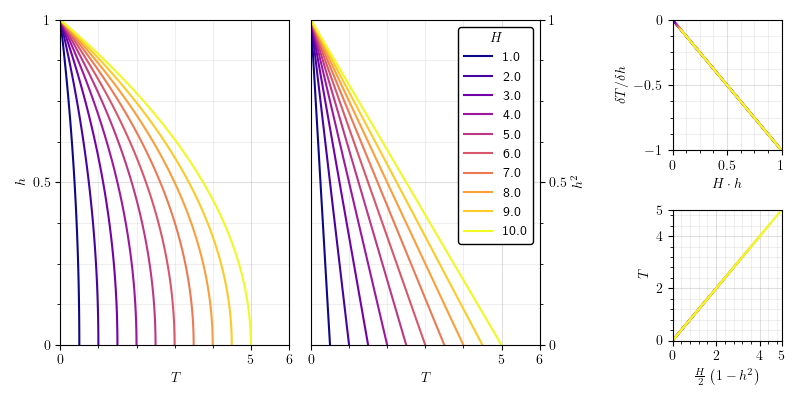
\includegraphics[width=0.7\linewidth]{files/7697321490a630ce259b3aa8db4668c0.png}

To provide some bounds on the expected behaviour of a mixed-heating model, it is helpful to review the effects of purely internal heating. Without the ability to arbitrarily specify a temperature scale, it is natural to use that which arises from pure conduction. Under a scenario of pure internal heating, the conductive geotherm is no longer linear, but scales with length squared \cite{Turcotte2014-by} \ref{isocondh}:

\begin{align*}
{{T(h)}_{c}}^{'} &= H\cdot h \\
\therefore {T(h)}_{c} &= \frac{H}{2} \left( 1 - h^2 \right)
\end{align*}

Where $H$ is the per-mass heating rate and $h$ is the dimensionless height from the base of the mantle. The maximum mantle temperature possible for a given value of $H$ is thus $H/2$. Because, at the outer boundary, the thermal flux is exactly $H$ (or, technically, $H \cdot \rho$ if dimensionalised), $H$ here is identical to the `conductive \textit{Nusselt} number', ${Nu}_{c}$.

Having obtained the conductive geotherm, we can select a nominal temperature scale:

\begin{equation}
{\Delta T}_H = \frac{\rho H b^2}{k}
\end{equation}

Where $k$ is the conductivity, $\rho$ is the density, $H$ is the per-mass heating rate, and $b$ is the characteristic spatial length. The temperature scale allows an `internally heated \textit{Rayleigh} number' ${\mathrm{Ra}}_H$ to be defined \cite{Roberts1967-aq}:

\begin{align*}
{\mathrm{Ra}}_H &= {\mathrm{Ra}}_B \cdot {\Delta T}_H \\
&= \frac{\alpha g \rho H b^5}{k \kappa \nu}
\end{align*}

Where ${\mathrm{Ra}}_B$ is the \textit{Rayleigh} number derived for basal heating, introducing the parameters of thermal expansivity $\alpha$, gravity $g$, thermal diffusivity $\kappa$, and momentum diffusivity $\nu$ \cite{Turcotte2014-by}. As in the basally-heated case, there exists for this number a critical value ${{\mathrm{Ra}}_{H}}_{\mathrm{cr}}$ which divides the purely conductive regime from the convecting regime \cite{Roberts1967-aq}:

\begin{equation}
{{\mathrm{Ra}}_{H}}_{\mathrm{cr}} \approx 868
\end{equation}

Usually we would be interested in deriving some scaling for the \textit{Nusselt} number with respect to ${\mathrm{Ra}}_H$. In this case, however, $Nu$ must always equal one. This follows because there are no other sources or sinks in the model except for $H$, which must be radiated in full from the upper boundary whether the interior is convecting or not. Rather than serving to augment the surface flux, convection in a purely internally-heated system only functions to smooth out interior temperatures. To describe this, we must choose a represenative internal temperature $T_{i}$, which should reflect a typical temperature in those regions where advection dominates \cite{Solomatov2000-xn}. Normalising $T_{i}$ by the true (measured) temperature scale $\Delta T$ gives ${T_{i}}^{*}$, the non-dimensional internal temperature, which then informs the definition of an `internal \textit{Rayleigh} number' ${\mathrm{Ra}}_i$:

\begin{equation}
{\mathrm{Ra}}_i = \frac{\alpha g {T_i}^{*} \Delta T b^3}{\kappa \nu}
\end{equation}

This observes, in other words, that - in an internally-heated system - the thermal contrast available to drive convection will always be less by some factor than the thermal contrast across the system as a whole.

While the flux across the upper boundary is fixed by the choice of parameter $H$, the actual geometry of the boundary that supplies this flux must be a function of the \textit{Rayleigh} number. At steady state, the interior temperature and the layer thickness adjust until a balance is reached, resulting in an outer temperature drop ${\Delta T}_o$ and outer boundary thickness ${\delta}_o$ that scale with, but are not solely determined by, the heating rate \cite{Schubert2001-ea}:

\begin{align*}
{\Delta T}_o &\propto \frac{H^{3/4}}{{\mathrm{Ra}}^{1/4}} \\
{\delta}_o &\propto \frac{1}{{(\mathrm{Ra}H)}^{1/4}}
\end{align*}

Wherein we observe that the implied flux (temperature drop divided by boundary thickness) remains equal to ${Nu}_c = H$, and hence $Nu=1$, as expected: all of that inner motion occurs without leaving any thermal trace on the surface.

By taking a boundary layer approach to the heat-producing regions \cite{Jaupart2010-zy} and exploiting certain known requisites of the purely conductive state \cite{Vilella2017-mg}, one can derive an alternative statement of the expected outer boundary layer properties in terms of the critical \textit{Rayleigh} number:

\begin{align*}
\frac{{\delta}_o}{h} &= {\left( \frac{{{\mathrm{Ra}}_{H}}_{\mathrm{cr}}}{{\mathrm{Ra}}_H} \right)}^{1/4} \\
\frac{{\Delta T}_o}{{\Delta T}_H} &= \frac{1}{2} \frac{{\delta}_o}{h}
\end{align*}

This relationship appears to hold empirically with good confidence \cite{Vilella2017-mg}.

Qualitatively, the addition of internal heating to the isoviscous convection problem imposes an asymmetry between upwellings and downwellings, which would otherwise be temperature-reversed mirrors of one another \cite{Weinstein1990-dd}. Because the thermal gradient of the conductive state rapidly drops with depth, the local \textit{Rayleigh} numbers of deeper layers can quickly become subcritical, such that a large portion of the domain from the base up is locked in a near-conductive state. At high $H$, large-scale motions cease, and only a thin sub-surface `mixing layer' witnesses any meaningful convection at all \cite{Parmentier1994-on}.

\paragraph{Mixed heating}

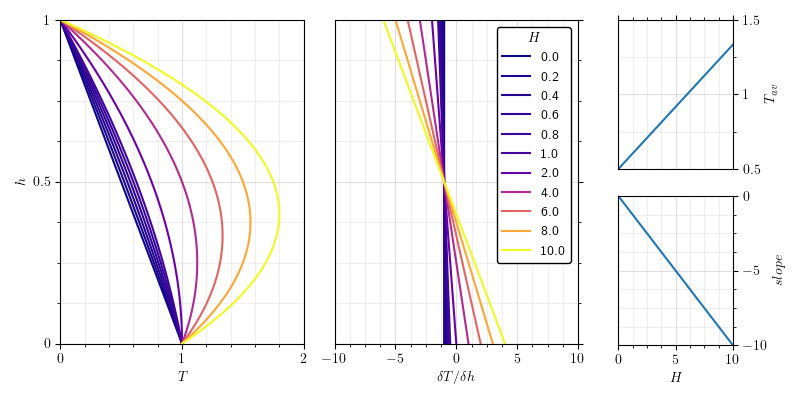
\includegraphics[width=0.7\linewidth]{files/545b6b3bb6664e7aace68e605ea8524a.png}

For systems driven by both internal and basal heating, the choice between basally-derived and internally-derived \textit{Rayleigh} numbers leads to ambiguity and confusion. One path forward is to define a dimensionless heating rate $H$ \cite{Schubert2001-ea}:

\begin{align*}
H &= {\mathrm{Ra}}_H / \mathrm{Ra} \\
&= \frac{\rho H^{*} D^2}{k {\Delta T}^{*}}
\end{align*}

The conventional basally-heated $\mathrm{Ra}$ derivation can then be used, with $H$ as a correcting coefficient.

While the purely internally-heated case has only one boundary layer (the outer), and the purely basally-heated case has symmetrical outer and inner boundaries, the mixed-heating case has two asymmetrical boundaries which are at least pseudo-independent of each other. While, at steady-state, the outer boundary flux is constrained to be always greater than the inner, the inner boundary flux may freely adjust itself as a function of the temperature differential between the prescribed lower boundary condition and the interior temperature. This intrinsic feedback makes quantitative analysis much more complicated.

As usual, a close consideration of the situation at the boundaries can set us on the right course. In the sorts of scenarios relevant to planetary settings, the lower boundary will remain hotter than the interior and the flux will be positive and substantial, in which case the outer boundary is required to transport the volumetric heating $H$ in addition to the basal heating \cite{Moore2008-je}:

\begin{align*}
{q}_{o} &\propto {\left| \frac{dT}{dh} \right|}_{h=1} \\
&\propto H + {q}_{i} \propto H + {\left| \frac{dT}{dh} \right|}_{h=0}
\end{align*}

Where ${q}_{o}$ and ${q}_{i}$ are the inner and outer heat fluxes.

At the limit where internal heating becomes negligible compared to the inner-outer temperature drop, internal heating can be ignored altogether and the system approximates a purely basally-heated model. At the opposite extreme, if the interior temperature due to internal heating is high enough, the inner flux may become negative, and the mantle will cool into the core: a case hard to envision in nature. Between these regimes is a transition point when the interior temperature becomes equal to the lower boundary condition. In this borderline case, the inner (core-mantle) flux is exactly zero (i.e. insulating), so that the mixed-heating system reproduces a purely internally-heated system. Thus, the mixed-heating model includes both internally-heated and basally-heated endmembers.

To sharpen this analysis, we can look at more closely at the conductive profile. While it is possible to derive this from first principles, it is more easily illustrated by a numerical approach \ref{isocondhmixed}. It is clear that the conductive geotherm forms a parabola whose second derivative is exactly equal to $-H$; the rest follows by integration, with the constants provided by logic and observation:

\begin{align*}
{{T(h)}_{c}}^{''} &= -H \\
{{T(h)}_{c}}^{'} &= -H \left( h - \frac{1}{2} \right) - 1 \\
{T(h)}_{c} &= \frac{Hh}{2} \left( 1 - h \right) - h - 1 \\
{{T}_{c}}_{av} &= \frac{H}{12} + \frac{1}{2}
\end{align*}

If each geotherm traces a parabola, a maximum `natural' temperature is implied where the first derivative is zero:

\begin{equation}
h_{T_{max}} = \frac{1}{2} - \frac{1}{H}, \quad H > 0
\end{equation}

If $h_{T_{max}}$ is less than zero for a particular value of $H$, then that maximum will never be realised and the true maximum temperature will be that at the mantle base, which is unit in our dimensionless treatment. The condition $h_{T_{max}} > 0$ thus represents the regime boundary between those conductive solutions that cool into the core and those that only cool into space. This occurs at exactly $H = 2$, or more generally:

\begin{equation}
H_{crit} = \frac{1}{{{T_{c}}_{av}}_{(H=0)}}, \quad \mathrm{Ra} < {\mathrm{Ra}}_{\mathrm{cr}}
\end{equation}

Where $H_{crit}$ is the critical heating factor above which the mantle cools into the core and at which the lower boundary becomes effectively insulating, as previously discussed.

If we define a `conductive \textit{Nusselt} number' - something of an oxymoron - we can see how the true \textit{Nusselt} number should be expected to scale:

\begin{align*}
{{Nu}_{c}}_{(mixed)} &= -{{T(h)}_{c}}^{'}, \quad h = 0 \\
&= 1 + \frac{H}{2} \\
&= {{Nu}_{c}}_{(basal)} + {{Nu}_{c}}_{(internal)}
\end{align*}

I.e. the surface flux in the mixed case is simply the sum of the two heat drivers considered separately, just as we would expect from first principles.

We now have an understanding of how the system behaves below the critical \textit{Rayleigh} number; now we must go above. One thing we can immediately observe from first principles is that the outer heat flux should be equal to the balance of $H$ and whatever flux, positive or negative, is occurring over the lower boundary:

\begin{equation}
{\phi}_o = H + {\phi}_i
\end{equation}

To analyse the mixed heating case, then, we need to invert our perspective and focus not on the outer boundary but on the inner boundary, whose core-ward temperature is equal to 1 and whose mantle-ward temperature - the `interior temperature' ${T_i}^{*}$ - is to be determined. Unfortunately, no universally accepted analytical treatment of ${T_i}^{*}$ post-convection has yet been devised.

One workaround starts with the interior temperature analytically obtained for a purely internally-heated system and modify it with empirical constants to accommodate the addition of basal heating \cite{Moore2008-je}:

\begin{equation}
T_i = 0.49 + 1.24 H^{3/4} {\mathrm{Ra}}^{-1/4}, \quad H < H_{inv}
\end{equation}

This scaling, however, is back-formed from an observed and arbitrary measurement of $T_i$ taken across the middle 60\% of a finite-element numerical model, and no justification for this particular choice is ventured nor defended across the range of $\mathrm{Ra}$ and $H$ values sampled.

Given a known value of $T_i$, the associated \textit{Nusselt} number should be proportional to that temperature drop divided by the stable outer boundary thickness ${\delta}_o$. Conventional boundary layer analysis can be used to argue a scaling of the form \cite{Schubert2001-ea}:

\begin{equation}
{\delta}_o = {\left( \frac{\mathrm{Ra}}{{\mathrm{Ra}}_{\mathrm{cr}}} \frac{\Delta T_b}{\Delta T} \right)}^{-1/3}
\end{equation}

Empirically, the same authors \cite{Moore2008-je} found that this scaling holds only for a much lower exponent of $\sim -0.303$ for $\mathrm{Ra}<=10^8$ and $H<10$, while apparently approaching the theoretical value with increasing $H$; the discrepancy was attributed to disruption by plumes from the lower boundary.

The next step is to attempt to derive the \textit{Nusselt}-\textit{Rayleigh} scaling, which we expect to approach the conventional power law behaviour under the \textit{beta} exponent $\beta = 1/3$. The expected relationship, however, does not manifest even approximately for the mixed heating case unless alternative definitions of $Nu$ and $\mathrm{Ra}$ are used. Subtracting the basal component from $Nu$ and using the arithmetic difference between $\mathrm{Ra}$ and ${\mathrm{Ra}}_{\mathrm{cr}}$ yields the following with some confidence \cite{Moore2008-je}:

\begin{equation}
Nu - 1 = \frac{H}{2} + 0.206 \cdot {\left( \mathrm{Ra} - {\mathrm{Ra}}_{\mathrm{cr}} \right)}^{0.318}
\end{equation}

While the above was calculated using a planar 2D model, an equivalent model suite in the spherical shell closely reproduced this relationship after geometry was accounted for \cite{Weller2016-nm}.

An alternative parameterisation \cite{Vilella2018-il} expresses $Nu$ in terms of the critical heating rate $H_{crit}$ after convection:

\begin{equation}
H_{crit} = 2 + 2 C_N {\left( \frac{\mathrm{Ra}}{{\mathrm{Ra}}_{\mathrm{cr}}} - 1 \right)}^{1/3}
\end{equation}

Where $C_N$ is an empirically-obtained constant argued to be exactly equal to 1.5. This definition of the convective $H_{crit}$ further defines two independent \textit{Nusselt} numbers depending on the magnitude of heating:

\begin{align*}
Nu &= \frac{1}{2} \left( H + H_{crit} \right), \quad &H \le H_{crit} \\
Nu &=  H - {\left( 2 \frac{{\Delta T}_{TBL,b}}{\Delta T} H \right)}^{1/2} \quad &H \ge H_{crit}
\end{align*}

Where ${\Delta T}_{TBL,b}$ is the temperature jump across the inner boundary layer, recalling that the mantle must cool into the core above $H_{crit}$.

\subsubsection{Isoviscous rheology in cylindrical geometry}

\paragraph{Defining a coordinate system}

In any convection model, gravity defines the natural down direction and gives us our first most important scale: the depth $z$ from the surface, or its complement, the height from the model base $h=1 -z$.

If the domain is allowed to curve around a certain locus, a cylindrical or annular geometry is obtained which is more appropriate for planetary mantles. While we retain $h$ and $z$ as terms relevant to any action within the domain, we must also introduce a concept of radial height $r$, understood here to represent the distance from the planetary centre of gravity. The cylindrical domain, for us representing the mantle, is thus bounded by the inner radius $r_{i}$ and the outer radius $r_{o}$, defining an area of $\pi(r_o^2 - r_i^2)$.

Our choice of radii implies a degree of curvature $f$:

\begin{equation}
f \equiv \frac{r_o}{r_i}
\end{equation}

Where $f=1$ is equivalent to an infinitely wide Cartesian box, $f\to0$ represents a full disk, and the values $\sim 0.5$ and $\sim 0.9$ would be appropriate for the whole mantle and upper mantle respectively. The ratio of radii $f$ is identical to the ratio of circumferences, so that $f=0.5$ represents a system where the arc length of the base is half that of the surface. (Note that this would imply infinite planetary radii at $f=1$ - hence the planar-like endmember $f=1$ is not strictly reachable under an assumption of curvature, though arbitrarily high values can be set to reproduce that behaviour \cite{Jarvis1993-cb}.)

If we further stipulate:

\begin{equation}
\Delta r = r_{o} - r_{i} = 1 \\
r_{o} \to 1 \quad as \quad f \to 0
\end{equation}

Then:

\begin{equation}
r_i = \frac{f}{1 - f}, \quad r_o = \frac{1}{1 - f} \\
r(h) = r_i + h
\end{equation}

Which suggests non-dimensionalising the planetary radial height $r$ as $r^{*}$ (\textit{r-star}) such that ${r^{*}}_o = 1$:

\begin{equation}
{r^{*}}_i = f, \quad {r^{*}}_o = 1 \\
\Delta r^{*} = 1 - f \\
r^{*}(h) = \frac{h + r_i}{r_0} = \frac{\Delta r^{*}}{r} = h(1-f) + f
\end{equation}

This leaves us with four different terms to describe radial position: $h$, the dimensionless height from the mantle base; $z$, its complement; $r$, the radial scale such that $r_o - r_i = 1$; and $r^{*}$, the radial scale such that $r_0 = 1$. Each of these scales will prove natural in some contexts and less so in others, and all find use in our analysis.

To complete our coordinate system, we require an angular coordinate as well: the angle $\theta$ in radians anticlockwise from an arbitrary origin. Often we will only want to reproduce a small wedge of the annulus, as time-dependence and numerical workload scale exponentially with aspect ratio; we can define our wedge selection $\Theta$ in radians:

\begin{equation}
\theta: 0 \to \Theta, \quad \Theta \leq 2\pi
\end{equation}

If the simulation is to represent periodic flow around the annulus, values of $\Theta$ must satsify $\pi / l$, where $l$ is a positive integer representing the number of convection cell pairs it would take to populate the full annulus at equivalent curvature (i.e. the number of upwellings or downwellings).

The selection of $\Theta$ also selects an aspect ratio for the domain, but only once we choose a depth at which to measure it. It is most convenient to use the arc length through the mid-depth, which then relates to $\Theta$ and $f$ via a new term: the radial distance from the planetary centre of gravity to the mantle mid-depth, $r_m$:

\begin{equation}
r_m \equiv \frac{r_{i} + r_{o}}{2} = \frac{1 + f}{2 \left( 1 - f \right)} \\
A = r_m \Theta
\end{equation}

If radius has been non-dimensionalised as above, this is equivalent to stating that the aspect ratio is equal to the area of the domain - regardless of $f$ - just as it is in the Cartesian case.

Such a scheme leaves us with two competing claims for a `natural' denominator of the angular coordinate - $\Theta$ and $r_m$. While authors have sometimes preferred to keep $\Theta$ and $r_m$ constant and allow $A$ to vary \cite{Jarvis1994-np}, we have for the most part chosen to fix $A$ and $r_m$ with $\Theta$ as the free parameter, as in \cite{Jarvis1993-cb}: this simplifies comparisons with plane-layer simulations at the cost of producing planforms which would be unstable if scaled to the full annulus.

Some system forcings, like internal heat, scale with area. The proportion of the annulus lying below a particular height $h$ - which we shall call $D$ for `disk' - is a function of the inner and mid-radii:

\begin{equation}
D(h) = \frac{r^2 - {r_i}^2}{2 r_m}, \quad r = h + r_i
\end{equation}

Having declared that the total area shall always equal the aspect ratio $A$, the true area under any depth $h$ is simply $D \cdot A$.

From $r_m$ we are also able to derive $s$, a statement of the angular length in `real' terms (i.e. in the same metric as $r$). It is convenient to non-dimensionalise $s$ as $s^{*} = s / A$, such that the dimensionless length through the mid-depth ${s^{*}}_m = 1$. We can then write $s^{*}$ very simply as a function of $r^{*}$, and the inner and outer lengths accordingly:

\begin{equation}
s^{*} = 2 \frac{r^{*}}{1+f} \\
{s^{*}}_i = 2 \frac{f}{1+f}, \quad {s^{*}}_o = 2 \frac{1}{1+f}
\end{equation}

The length $s$ is, among other things, the factor by which an average measurement of some variable taken across a layer can be converted into a total value for that layer. It is vital to account for varying $s$ whenever comparing between different layers in a given system, or between equivalent layers in systems of differing $f$.

\paragraph{Basal heating}

\subparagraph{Conductive solution}

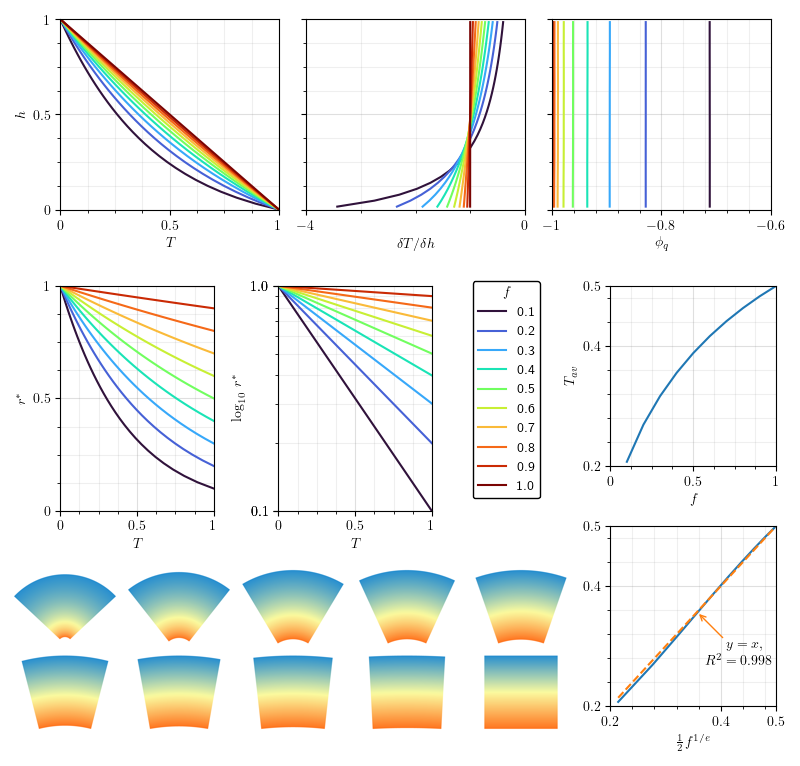
\includegraphics[width=0.7\linewidth]{files/7f673a8edbf6184fb731e1f10b346ed0.png}

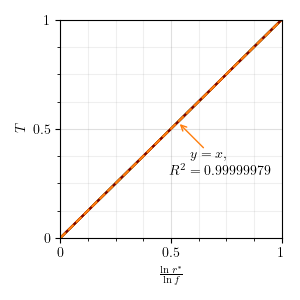
\includegraphics[width=0.7\linewidth]{files/1fa833915eb9bd27a143f7b2082136f6.png}

It is a requirement of a conductive steady state ($Nu=1$) that the thermal flux must be the same through every layer. In the planar case this results in a linear geotherm which, in a model with fixed and unitless boundary temperatures, results in a simple function of $T = z$ where $z$ is dimensionless depth from the top of the model. The average temperature is then trivially $T_{av}=0.5$. (For any system in pure conduction the \textit{Nusselt} number is by definition 1.)

In a cylindrical domain, however, the length of each layer $s$ is a function of depth and curvature as we have shown; consequently, shallower layers may transmit the same flux with a smaller temperature drop:

\begin{equation}
\phi_q \propto s \cdot \frac{dT}{dh}
\end{equation}

To define the flux, we need the geothermal gradient. The conductive geotherm can be elegantly stated in terms of $r^{*}$ \ref{isocondf} \ref{isocondffit}:

\begin{equation}
T(h) = \frac{\ln{r^{*}}}{\ln{f}}
\end{equation}

And so the geothermal gradient:

\begin{equation}
\frac{dT}{dh} = \frac{f-1}{r^{*}\ln{f}}
\end{equation}

And finally the flux itself can be written as:

\begin{align*}
\phi_q &\propto \frac{s^{*}(f-1)}{r^{*}\ln{f}} \\
&= \frac{2(1-f)}{(f+1)\ln{f}}
\end{align*}

\begin{align*}
&\to -1 &as \quad f \to 1 \\
&\to 0 &as \quad f \to 0
\end{align*}

Or very succinctly in terms of the `true' radius of the mid-depth:

\begin{equation}
\phi_q \propto \frac{1}{r_m \ln{f}}
\end{equation}

To facilitate comparison between systems of different curvature, we can then use the above to define a dimensionless planetary flux ${\phi_q}^{*}$ - which is really just another name for the \textit{Nusselt} number $Nu$:

\begin{align*}
{\phi_q}^{*} &= \frac{ {\phi_q} }{ {\phi_q}_c } \\
&\equiv Nu
\end{align*}

Where the subscript $c$, here and elsewhere, denotes a purely conductive endmember. Because $Nu$ now inherits a dependency on $f$, it is no longer equivalent to the dimensionless surface temperature gradient, and so it is important always to present and discuss it in its proper terms as a ratio of fluxes.

Just as the flux now scales with $f$, so must the average mantle temperature. In the planar case, the average temperature of the system is always half the temperature drop. In the cylindrical case, however:

\begin{align*}
T_{av} &= \dfrac{1}{2} \large{\root \huge{e} \of f} \\
&\equiv T_{c}
\end{align*}

The relationship is apparent in the numerical results \ref{isocondf}.

\subparagraph{Instability and convection}

An implication of $Nu$'s dependency on curvature is that the upper and lower boundaries must no longer be symmetrical. This invalidates many of the assumptions that made the planar case amenable to analysis. The additional space at the top of the model now allows more room for downwellings relative to basal upwellings, tending to promote instability \cite{Jarvis1991-ir}; on the other hand, the curved geotherm and the increased surface for radiating heat would tend to permit a comparatively thicker upper boundary layer. The effect of these countervailing forcings on the fundamental scalings of $Nu$, $Ra$, $Ra_{cr}$, and the all-important relation $Nu \propto R^{\beta}$ is not obvious.

To begin to unpack the complexities of convection in the annulus, we can start with the assumption that - as in the planar case - the convective steady state will eventually result in a broad intracellular region of uniform temperature $T_{cell}$. Assuming a unit temperature drop $\Delta T = 1$, we can write:

\begin{align*}
{\Delta T}_o &= T_{cell} \\
{\Delta T}_i &= 1 - T_{cell}
\end{align*}

Knowing that the inner and outer fluxes ${\phi_q}_i$ and ${\phi_q}_o$ must be equal at steady state, and that the outer boundary - due to its greater length - can sustain that flux with a gradient shallower by a factor of $f$, we can deduce a relation between the outer and inner thermal gradients, and thence between $T_{cell}$ and the inner and outer boundary layer thicknesses ${\Delta r}_i$ and ${\Delta r}_o$:

\begin{align*}
f \frac{{\Delta T}_i}{{\Delta r}_i} &= \frac{{\Delta T}_o}{{\Delta r}_o} \\
\frac{{\Delta r}_i}{{\Delta r}_o} &= f \frac{1 - T_{cell}}{T_{cell}}
\end{align*}

For each of the two layers, we can prescribe a layer-specific \textit{Rayleigh} number accordingly:

\begin{align*}
Ra_o &\propto T_{cell} {{\Delta r}_o}^3 \\
Ra_i &\propto (1 - T_{cell}) {{\Delta r}_i}^3
\end{align*}

Having maintained non-dimensionality throughout, it is simple relate these two boundary \textit{Rayleigh} numbers to the bulk $Ra$ value:

\begin{equation}
Ra_{layer} = Ra \cdot {\Delta T}_{layer} \cdot {{\Delta r}_{layer}}^3
\end{equation}

At this point, however, we have exhausted the insight we can obtain without making further assumptions. If we provide that the inner and outer boundary thicknesses must be the same, as they are in the planar case, we can see that:

\begin{equation}
T_{cell} = \frac{f}{f + 1} \quad \leftarrow {\Delta r}_i = {\Delta r}_o
\end{equation}

This, however, would imply that the inner and outer \textit{Rayleigh} numbers are divergent. If we instead choose to conserve $Ra$, then: (\cite{Jarvis1993-cb})

\begin{equation}
T_{cell} = \frac{1}{1 + f^{-3/4}} \quad \leftarrow Ra_i = Ra_o
\end{equation}

Both possibilities converge on 0.5 when $f\to1$ and 0 when $f\to0$, as we would expect.

However it is estimated, it is clear that, as $Ra$ increases and boundaries thin, more of the mantle will fall in the intracellular region and global temperatures as a whole will approach $T_{cell}$. Conversely, if $Ra$ slips below its critical value, the boundary layers will disapper and the entire domain will enter the conductive regime: $T^{av} = T_{c}$. These two temperatures therefore make up respectively the lower and upper endmembers of global temperature:

\begin{align*}
T_{av} &\approx T_{c}, \quad Ra < Ra_{cr} \\
&\to T_{cell}, \quad Ra \to \infty
\end{align*}

It makes intuitive sense that the effect of increasing $Ra$ should be to decrease global temperatures, since that is exactly why convection is preferred wherever possible - though this intuition may not hold for all rheologies.

Of course, what we desire most of all is a cylindrical scaling for the mantle convection power law $Nu \propto R^{\beta}$. Following \cite{Jarvis1993-cb} and mandating equality of inner and outer $Ra_{layer}$, it is possible to construct a `geometric correction' $g(f)$ that functions as a coefficient of the \textit{beta} scaling:

\begin{equation}
g(f) = \frac{Nu_{c}}{{T_{cell}}^{4/3}} \quad \leftarrow Ra_i = Ra_o \\
Nu = g(f) \cdot R^{\frac{1}{3}}
\end{equation}

Using this scaling, Jarvis was able to obtain a \textit{beta} exponent of $0.321 \pm 0.001$ across four values of $f$ from $(1.0 - 0.1)$ \cite{Jarvis1993-cb}.

\paragraph{Internal heating in the annulus}

\subparagraph{Conductive solution}

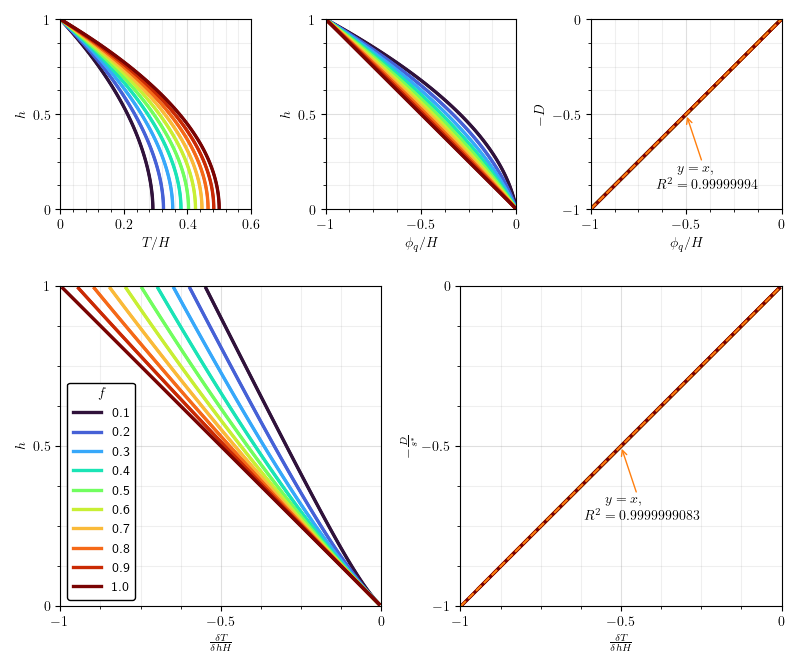
\includegraphics[width=0.7\linewidth]{files/0a5abf12a1f99d470b669652116b36ed.png}

It was established previously that, for an internally heated system, the geotherm and geothermal gradient are represented by:

\begin{align*}
{T(h)}_{c(internal)} &= \frac{H}{2} \left( 1 - h^2 \right) \\
{{T(h)}_{c(internal)}}^{'} &= H\cdot h
\end{align*}

This is intuitive because the source flux visible to each layer is proportional to the area below that layer, which goes linearly with height $h$ in a planar domain.

In the annulus, though, the proportion of the domain beneath a given height $h$ is instead represented by $D$, as we have shown. If we further assume that $H$ is non-dimensionalised so as to represent the total flux of the model (i.e. it equals 1 for all geometries), then the flux through each layer height $h$ of the annulus must simply be:

\begin{equation}
{\phi_q}(h) = -H \cdot D(h)
\end{equation}

We show that this holds exactly \ref{isocondinternal}.

As before, the geothermal gradient required to transmit this flux must account for the varying layer length $s^{*}$ - a function of $h$ and the $f$ parameter. Thus:

\begin{equation}
\frac{dT}{dh} \propto \frac{\phi_q}{s^{*}} = -\frac{HD}{s^{*}}
\end{equation}

The integral with respect to $h$ yields the geotherm:

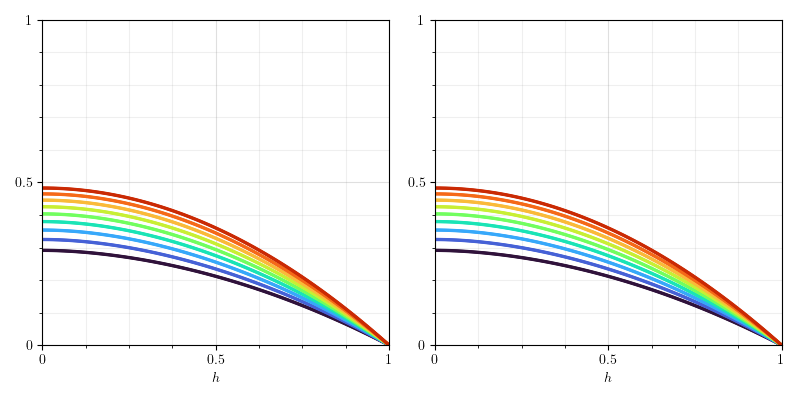
\includegraphics[width=0.7\linewidth]{files/f584a98f5b3d859cd64a1a5095d25dd2.png}

\paragraph{Mixed heating in the annulus}

\subparagraph{Conductive solution}

\subsubsection{Conclusion}

\subsection{Methods}

\subsection{Results}

\subsection{Discussion}

\subsection{Conclusion}

\section{Temperature-dependant rheology}

\section{Viscoplastic rheology}

\section{New techniques}

\section{Discussion}


\bibliography{main.bib}

\end{document}
